\documentclass[a4paper]{article}
\usepackage[utf8]{inputenc} % standard unicode
\usepackage[english]{babel} % corretta sillabazione in inglese
\usepackage{geometry} % per impostare margini e layout pagina
\usepackage{amssymb} % per l'ambiente matematico
\usepackage{amsmath} % per l'ambiente matematico
\usepackage{enumitem} % per elenchi puntati
\usepackage{multirow} % per celle che si espandono su più righe
\usepackage{tabularx} % per tabelle con larghezza flessibile
\usepackage[table]{xcolor} % per colorare le tabelle
\usepackage{booktabs} % per linee orizzontali tabelle
\usepackage{hyperref} % per collegamenti
\usepackage{graphicx} % per immagini
\usepackage{listings} % per codice
\usepackage{xcolor} % per colori
\usepackage{tikz} % per disegnare bayesian network
\usepackage{circuitikz} % per disegni di circuiti elettrici

% definizione colori per codice
\definecolor{codegreen}{rgb}{0,0.6,0}
\definecolor{codegray}{rgb}{0.5,0.5,0.5}
\definecolor{codepurple}{rgb}{0.58,0,0.82}
\definecolor{backcolour}{rgb}{0.95,0.95,0.92}

% definizione stile codice
\lstdefinestyle{mystyle}{
	language=C++,
	morekeywords={constexpr,string,C_style_cast,noexcept,alignof,std,wait,signal,acquire,release},
	emph={int,char,double,float,unsigned,string,vector,initializer_list,semaphore},
	backgroundcolor=\color{backcolour},    % sfondo
	commentstyle=\color{codegreen},        % commenti
	keywordstyle=\color{magenta},          % keywords
	identifierstyle=\color{blue},          % variabili
	stringstyle=\color{codepurple},        % stringhe
	directivestyle={\color{purple}},       % direttive
	emphstyle={\color{magenta}},           % tipi
	numberstyle=\tiny\color{codegray},     % numeri
	basicstyle=\ttfamily\footnotesize,
	breakatwhitespace=false,
	breaklines=true,
	captionpos=b,
	keepspaces=true,
	numbers=left,
	numbersep=-12pt,
	showspaces=false,
	showstringspaces=false,
	showtabs=false,
	tabsize=4
}

% utilizzo stile codice
\lstset{style=mystyle}
\lstset{literate={~} {{\raisebox{0.4ex}{\texttildelow}}}{1}}

% per margini
\geometry{a4paper,left=25mm, right=25mm, bottom=25mm, top=30mm}

% per centrare testo nelle tabelleX
\renewcommand\tabularxcolumn[1]{m{#1}}
\newcolumntype{L}{>{\raggedright\arraybackslash}X}
\newcolumntype{C}{>{\centering\arraybackslash}X}
\newcolumntype{R}{>{\raggedleft\arraybackslash}X}

% per elenchi puntati
\setlist[itemize]{label=-, partopsep=0pt, topsep=3pt, itemsep=0pt}
\setlist[enumerate]{partopsep=0pt, topsep=3pt, itemsep=0pt}

% percorso delle immagini da inserire
\graphicspath{{./}}

% per disegni
\usetikzlibrary{positioning, shapes.geometric, arrows.meta, calc}


\title{Microelectronics laboratory notes}
\author{Giacomo Simonetto}
\date{Second semester 2025-26}

\begin{document}

\maketitle
\begin{abstract}
	Microelectronics laboratory notes for the second semester of the academic year 2025-26 at the University of Padua.
\end{abstract}

\newpage

\tableofcontents

\newpage

\section{Prototyping techniques}
\subsection{PCB and PCA}
\subsubsection*{Difference between PCB and PCA}
\begin{itemize}
	\item \textbf{PBC - Printed Circuit Board}: only the surface with conductive pads for mounting electronic components, tracks
	or traces, called metal lines, to connect the components, and via holes to connect different layers of the PCB or to mount
	components with through-hole technology
	\item \textbf{PCA - Printed Circuit Assembly}: a PCB with electronic components mounted on it
\end{itemize}

\subsubsection*{PCB classification}

\begin{itemize}[itemsep=5pt]
	\item classification based on \textbf{substrate materials}:
	\begin{itemize}[topsep=0pt]
		\item \textbf{FR-4}: organic composite rigid material made on fiberglass cloth wth an epoxy resin binder, it is rigid,
		flame resistant and supports up to 135°C temperatures
		\item \textbf{ceramic}: rigid inorganic ceramic substrate (Al\(_2\)O\(_3\), AlNi, \dots) for better performance at high
		frequencies and thermal conductivity
		\item \textbf{metal core}: metal core under the substrate (copper or aluminum) for better heat dissipation
		\item \textbf{flexible substrates}: flexible materials for applications where the PCB can be bent or folded
	\end{itemize}
	\item classification based on \textbf{physical nature}:
	\begin{itemize}[topsep=0pt]
		\item \textbf{rigid}: made of solid materials that do not bend
		\item \textbf{flexible}: made of materials that can bend without breaking (for wearable devices, \dots)
		\item \textbf{rigi-flex}: combination of rigid and flexible sections in the same PCB, usually flex parts are used
		for interconnections between rigid sections (FFC - flat flexible cables)
	\end{itemize}
	\item classification based on \textbf{number of layers}:
	\begin{itemize}[topsep=0pt]
		\item \textbf{single-sided}: only one layer of conductive tracks, components mounted on the same side
		\item \textbf{double-sided}: two layers of conductive tracks, components can be mounted on both sides
		\item \textbf{multi-layer}: more than two layers of conductive tracks, components can be mounted on both sides, used for complex circuits
	\end{itemize}
	\item classification based on \textbf{production methods of the conductive pattern}:
	\begin{itemize}[topsep=0pt]
		\item \textbf{discrete conductor pattern}: conductive tracks are printed by depositing conductive material directly
		on the substrate without using a lithographic imaging process
		\item \textbf{graphic conductor pattern}: tracks are printed using a photographic process (deposit, photoresist,
		UV exposure, etching) to obtain finer and more precise patterns
	\end{itemize}
\end{itemize}

\subsubsection*{Component classification}
\begin{itemize}[itemsep=5pt]
	\item classification based on \textbf{mounting technology}:
	\begin{itemize}[topsep=0pt]
		\item \textbf{TH - Through-Hole}: components with leads or pins that go through holes in the PCB
		\item \textbf{SMT - Surface-Mount}: components that are soldered directly on the surface of the PCB
	\end{itemize}
	\item classification based on \textbf{package types}:
	\begin{itemize}[topsep=0pt]
		\item \textbf{DIP - Dual Inline Package}: TH package with two parallel pin rows, with 100 mil pitch
		\item \textbf{SOP - Small Outline Package}: SMT package with no pins and 25 mil pitch
		\item \textbf{SSOP - Shrink SOP}: SMT package smaller than SOP
		\item \textbf{TSSOP - Thin SSOP}: SMT package smaller than SSOP
		\item \textbf{DQNF - Dual Quad Flat No-leads}: SMT package soldered with pads or balls
	\end{itemize}
\end{itemize}

\vspace{5pt}

\textbf{Pitch} is the distance between two adjacent pins or leads of a component. It is measured in mils:
\[1 \; \text{mil} \; = \; \frac{1}{1000} \; \text{inch} \; = \; 0.0254 \;\text{mm}\]


\subsubsection*{SMT assembly process}
\begin{enumerate}[itemsep=0pt]
	\item \textbf{setup}: preparation of the PCB and components for assembly
	\item \textbf{screen print}: application of solder paste on the PCB pads using a stencil
	\item \textbf{SMT placement}: placement of components on the PCB using a pick-and-place machine
	\item \textbf{reflow}: heating the PCB to melt the solder paste and create permanent connections between components and PCB pads
	\item \textbf{hand assembly}: manual placement of components that cannot be placed by the machine (large through-hole components, \dots)
	\item \textbf{wave solder}: soldering of through-hole components by passing the PCB over a wave of molten solder
	\item \textbf{final assembly}: manual assembly of remaining components and final checks
	\item \textbf{wash}: cleaning of the PCB to remove flux residues and contaminants
	\item \textbf{circuit test}: testing components and connections to ensure proper functionality
	\item \textbf{stress test}: testing the PCB under extreme conditions (temperature, humidity, \dots)
	\item \textbf{functional test}: testing the PCB in real operating conditions to verify that it performs as expected
	\item \textbf{pack/ship}: packaging and shipping of the assembled PCB to customers or distributors
\end{enumerate}

\subsection{Resistors}
\subsubsection*{Resistor color code}
Resistor values are indicated with color bands on the resistor body. The first two bands on the left represent digits, the
third band is a multiplier, the fourth band indicates the tolerance of the resistor value. The color code is as follows:

\begin{table}[h]
	\centering
	\newcommand{\cbox}[1]{\textcolor{#1}{\rule[-0.1cm]{0.4cm}{0.4cm}}}
	\renewcommand{\arraystretch}{1.1}

	\definecolor{gold}{RGB}{255, 215, 0}
	\definecolor{silver}{RGB}{192, 192, 192}

	\begin{tabular}{|l|c|c|c|c|c|c|}
		\hline
		\(\;\;\;\) \textbf{Color} & \textbf{1st Band} & \textbf{2nd Band} & \textbf{3rd Band Multiplier} & \textbf{4th Band Tolerance} \\
		\hline
		\cbox{black} \(\;\) \textcolor{black}{Black} & 0 & 0 & $\times \; 1 \; \Omega$ & \\
		\hline
		\cbox{brown} \(\;\) \textcolor{black}{Brown} & 1 & 1 & $\times \; 10 \; \Omega$ & $\pm \; 1\%$ \\
		\hline
		\cbox{red} \(\;\) \textcolor{black}{Red} & 2 & 2 & $\times \; 100 \; \Omega$ & $\pm \; 2\%$ \\
		\hline
		\cbox{orange} \(\;\) \textcolor{black}{Orange} & 3 & 3 & $\times \; 1 \; \text{k}\Omega$ & \\
		\hline
		\cbox{yellow} \(\;\) \textcolor{black}{Yellow} & 4 & 4 & $\times \; 10 \; \text{k}\Omega$ & \\
		\hline
		\cbox{green} \(\;\) \textcolor{black}{Green} & 5 & 5 & $\times \; 100 \; \text{k}\Omega$ & $\pm \; 0.5\%$ \\
		\hline
		\cbox{blue} \(\;\) \textcolor{black}{Blue} & 6 & 6 & $\times \; 1 \; \text{M}\Omega$ & $\pm \; 0.25\%$ \\
		\hline
		\cbox{violet} \(\;\) \textcolor{black}{Violet} & 7 & 7 & $\times \; 10 \; \text{M}\Omega$ & $\pm \; 0.10\%$ \\
		\hline
		\cbox{gray} \(\;\) \textcolor{black}{Grey} & 8 & 8 & $\times \; 100 \; \text{M}\Omega$ & $\pm \; 0.05\%$ \\
		\hline
		\cbox{white} \(\;\) \textcolor{black}{White} & 9 & 9 & $\times \; 1 \; \text{G}\Omega$ &  \\
		\hline
		\cbox{gold} \(\;\) \textcolor{black}{Gold} & & & $\times \; 0.1 \; \Omega$ & $\pm \; 5\%$ \\
		\hline
		\cbox{silver} \(\;\) \textcolor{black}{Silver} & & & $\times \; 0.01 \; \Omega$ & $\pm \; 10\%$ \\
		\hline
	\end{tabular}
\end{table}

\vspace{-15pt}

\subsubsection*{E-series}
Resistors values are standardized in the E-series, where the number \(n\) after ``E'' indicates the number of values per decades
distributed logarithmically: \(\text{step size} = 10 ^ {1/n}\). The most common series are:
\begin{itemize}
	\item \textbf{E6}: 6 values per decade, 20\% tolerance, 47\% step size, 2 digit bands
	\item \textbf{E12}: 12 values per decade, 10\% tolerance, 21\% step size, 2 digit bands
	\item \textbf{E24}: 24 values per decade, 5\% tolerance, 10\% step size, 2 digit bands
	\item \textbf{E48}: 48 values per decade, 2\% tolerance, 5\% step size, 3 digit bands
	\item \textbf{E96}: 96 values per decade, 1\% tolerance, 2.5\% step size, 3 digit bands
	\item \textbf{E192}: 192 values per decade, 0.5\% / 0.25\% / 0.10\% tolerance, 1.23\% step size, 3 digit bands
\end{itemize}

\noindent
In the laboratory we use E12 resistors, the most common and widely available. If the required value is not available in the E12
series, we can combine resistors in series or parallel to obtain the desired value.

\subsection{Capacitors}
\subsubsection*{Ceramic capacitors}
Ceramic capacitors are made with one or more layers of ceramic dielectric material coated by silver plates. They are small, cheap,
with low capacitance values and not polarized. They are used for decoupling and filtering DC and AC signals. Capacitance values are
indicated in \(pF\) with a three-digit code:
\begin{itemize}
	\item the first two digits represent the significant figures of the capacitance value
	\item the third digit indicates the number of zeros to add to the values
\end{itemize}
For example, a capacitor with code ``103'' has a capacitance of \(10 \times 10^3 \; pF = 10 \; nF\).

\subsubsection*{Film capacitors}
Film capacitors are made with a thin plastic film (polyester, polystyrene, polypropylene, polycarbonate, metalized paper, Teflon,
\dots) as dielectric material  that separates the two electrode layers made of metal foils (zinc or aluminum) sometimes applied
directly to the dielectric film. By having a wide surface area, they can achieve higher capacitance values from \(5 \; pF\)
to \(100 \; \mu F\). They have low tolerance, good reliability and high temperature ratings. They come in different shapes
and sizes, normally in rectangular forms.

\subsubsection*{Electrolytic capacitors}
Electrolytic capacitors are made of a metal oxide film (aluminum) as dielectric material, covered by an electrolyte solution
on one side as a second dielectric layer. Both layers are coupled with two aluminum foils as electrodes and sealed in a cylindrical
aluminum case. They can achieve very high capacitance values and are used for low frequency, power supplies and decoupling applications.
They are polarized, with the positive terminal connected to the aluminum oxide layer. If they are connected in reverse, the oxide
layer can break down and cause the capacitor to fail.

\subsection{Integrated circuits}
Integrated circuits (ICs) are electronic components that contain multiple transistors, diodes, resistors and capacitors
inside the same package. In the laboratory we use ICs in DIP packages, which are easy to handle and mount on breadboards.
Every IC has a notch or a dot to indicate the position of pin 1 and to orient the component correctly.

\subsection{Breadboards}
Breadboards are prototyping tools that allow to build and test electronic circuits without soldering. They are made of two
horizontal rails or buses usually used for power supply connections, and a grid of vertical connected holes for mounting
components and making connections. 

\subsection{Software for prototyping circuits}
\subsubsection*{Common prototyping software}
\begin{itemize}
	\item \textbf{Fritzing}: design circuits on a virtual breadboard and simulate their behavior
	\item \textbf{LTspice}: simulate electronic circuits and analyze their behavior
	\item \textbf{Fusion PCB}: prototype and design PCBs
\end{itemize}

\subsubsection*{Circuit simulation}
Circuit study consist in solving first order equations and trascurating noise, temperature, parassitic capacitance,
channel length modulation, \dots ~ Computer aided simulations are useful to observe the behavior of circuits
considering also second/third order effects and non-idealities by solving matematical models of the componets provided
by the manufacturer. Circuit study and design is still required to understand the behavior of the circuit and understand
simulation results.

\section{Laboratory instrumentation}
\subsection{Oscilloscope}
\subsubsection*{Introduction}
An oscilloscope is an electronic instrument that displays electrical signals graphically as a voltage versus time plot. Some common
use cases of oscilloscopes include:
\begin{itemize}
	\item \textbf{wave shape}: observing the shape of electrical signals
	\item \textbf{amplitude}: measuring the voltage levels of signals
	\item \textbf{frequency}: measuring the frequency of periodic signals
	\item \textbf{time between events}: measuring the time interval between two events in a signal
	\item \textbf{AC/DC components}: analyzing the DC and AC components of signals
	\item \textbf{noise}: detecting and analyzing noise in electrical signals
\end{itemize}

\subsubsection*{Oscilloscope architecture}
\begin{itemize}
	\item \textbf{input coupling}: switch that add a capacitor in series to the input signal to block the DC component and only
	let the AC component pass through, it is often used to isolate the AC signal from the DC offset and to analyze the AC
	characteristics of the signal
	\item \textbf{amplitude control}: amplifier/attenuator that adjusts the amplitude of the input signal to provide a
	suitable voltage range for the analog-to-digital converter (ADC)
	\item \textbf{channel isolation}: optical (with photodiodes) or galvanic (with transformers) isolation to isolate the input
	signal from the internal circuitry of the oscilloscope and to prevent interference and damage to the device
	\item \textbf{Analog to Digital Converter (ADC)}: samples the analog input signal at regular intervals and converts it into
	digital values for processing and display in real time
	\item \textbf{memory}: stores the digital values of the signal for processing and display
	\item \textbf{processor}: manage the sample storage in memory, processes the digital values of the signal to perform various
	functions such as triggering, measurement, graphics processing, \dots and controls the user interface
	\item \textbf{triggering}: digital elaboration of the input signal to detect specific events (rising edge, falling edge,
	edge delay, pulse width, n-cycles, \dots) and align the signal on the screen based on the detected events
\end{itemize}

\subsubsection*{Oscilloscope performances}
\begin{itemize}
	\item \textbf{bandwidth}: the frequency range of the oscilloscope, measured in MHz; the upper limit is the frequency at which
	a sinusoidal signal is attenuated by 3 dB (about 70.7\% of the original amplitude); it is recommended to use an oscilloscope
	with a bandwidth at least 5 times higher than the frequency of the signal to be measured to ensure accurate
	reproduction of the signal 
	\item \textbf{sampling rate}: the number of samples taken per second to reconstruct the input signal; as for bandwidth, it is
	recommended to have a sampling rate at least 5 times higher than the frequency of the signal to be measured
	\item \textbf{record length}: the number of samples that can be stored in memory for analysis and display; it determines the
	maximum time interval that can be observed on the oscilloscope screen at maximum sampling rate, obtained by the formula: 
	\(\textit{acquired time} = \textit{record length} \; / \; \textit{sampling rate}\); if the time window is bigger than the
	acquired time, the oscilloscope will automatically reduce the sampling rate to fit the signal in the time window, which can
	result in a loss of detail and accuracy in the signal representation
\end{itemize}
NOTE: the oscilloscope acquisition is not continuous, it has a dead time between acquisitions during which the oscilloscope
is busy to flush the memory and prepare for the next acquisition.

\subsubsection*{Oscilloscope control panel}
\begin{itemize}
	\item \textbf{channel inputs}: BNC connectors (coaxial cables) for connecting probes to the oscilloscope
	\item \textbf{volts/div}: adjust the vertical scale of the signal on the screen, it determines how many volts are represented
	by each vertical grid division
	\item \textbf{vertical position}: adjust the vertical position of the signal on the screen, it allows to move the signal up
	or down to align it with the grid or to compare it with other signals
	\item \textbf{time/div}: adjust the horizontal scale of the signal on the screen, it determines how much time is represented
	by each horizontal grid division
	\item \textbf{horizontal position}: adjust the horizontal position of the signal on the screen, it allows to move the signal
	left or right to align it with the grid or to compare it with other signals
	\item \textbf{trigger level}: adjust the voltage level at which the oscilloscope triggers and starts the acquisition of the
	signal
	\item other controls for trigger options, coupling, autoscale, cursors, math functions, \dots
\end{itemize}

\subsubsection*{Oscilloscope display}
The oscilloscope display is divided into a grid of horizontal and vertical divisions, which are used to measure the amplitude
and time of the signal. The vertical divisions represent voltage levels, while the horizontal divisions represent time intervals.
There are also indicators for:
\begin{itemize}
	\item \textbf{waveform markers}: horizontal line that indicates the 0 V level on the screen for every channel
	\item \textbf{waveform position}: vertical line that indicates the zero time point on the screen (where the trigger event occurs)
	\item \textbf{cursors}: vertical and horizontal lines that can be moved by the user to measure voltage levels and time intervals
	\item \textbf{div settings}: indicators for the current volts/div and time/div settings for each channel
	\item other indicators for general settings, measurements, information, \dots
\end{itemize}

\subsubsection*{Triggering}
Triggering is a feature of the oscilloscope that allows to horizontally align the signal on the screen by positioning the zero time
point at a specific event in the signal. The trigger can be set to detect different types of trigger events, such as:
\begin{itemize}
	\item \textbf{rising edge}: when the voltage level becomes greater than a specified threshold
	\item \textbf{falling edge}: when the voltage level becomes smaller than a specified threshold
	\item \textbf{edge delay}: after a specified time delay from the rising or falling edge
	\item \textbf{pulse width}: when the signal pulse width is greater or smaller than a specified value
	\item \textbf{n-cycles}: after a specified number of cycles of the signal
	\item \textbf{digital patterns}: recognize typical patterns of  digital protocols (I2C, SPI, CAN, USB, \dots)
\end{itemize}
NOTE: it is not possible to trigger two signals at the same time, if two signals have different frequencies, only one of them will
be triggered and correctly displayed on the screen.

\subsubsection*{Cursors}
Cursors are vertical and horizontal lines that can be moved by the user to measure voltage levels and time intervals on the
oscilloscope display. They can be used to measure amplitude, frequency, period, rise time, fall time, duty cycle, \dots of
the signal. It is a more accurate measurement method compared to counting the number of divisions on the grid.

\subsubsection*{Acquisition mode}
There are different acquisition modes that determine how the oscilloscope samples and processes the input signal. Particularly
important is the \textbf{average mode}, which takes multiple acquisitions of the signal and displays an average of them to filter
high frequency noise and improve the signal quality. Note that the average mode slow down the acquisition process.

\subsubsection*{AC/DC coupling}
The AC/DC coupling switch allows to add a capacitor in series to the input signal to filter out the DC component. This
is useful to analyze the AC characteristics of the signal without being affected by the DC offset. It is important to
note that when the signal frequency is too low, the capacitor starts to filter out low frequencies (10-20 Hz) that are
part of the AC signal, causing voltage ``droop'' or ``sag'' in the waveform. In general it is recommended to use AC coupling
for signals with frequencies over 50-200 Hz.

\subsubsection*{Input impedance and amplification/attenuation stage}
In normal working conditions, the input impedance of the oscilloscope is set to HiZ (high impedance) with a value of
\(1 \; M\Omega\). Some oscilloscopes can also have a low impedance setting (LoZ) with a value of \(50 \; \Omega\) that
bypasses the conditioning stage and directly connects the input signal to the ADC. This setting is useful for measuring
high frequency signals but it can cause damage to the oscilloscope if the input voltage is bigger than 5 V.

\subsection{Function generator}
\subsubsection*{Introduction}
A function generator is an electronic instrument that generates electrical waveforms of adjustable shapes, frequencies and
amplitudes. It acts as an AC voltage source in series with a DC offset voltage source and an internal resistance.

\subsubsection*{Output impedance}
The output impedance of a function generator is \(50 \; \Omega\) and the instrument expects to be connected to a load with
the same impedance. For this reason the real output voltage is doubled to ensure the desired voltage across the load. When
the function generator is connected to a load with a different impedance, the load impedance must be set accordingly. In
particular, when it is connected to a HiZ load, the instrument must be set to HiZ mode.

\subsection{Multimeter}
The multimeter is an electronic instrument that can measure voltage, current and resistance. It is used to measure a wide
voltage/current range with high accuracy. 

\subsection{Power supply}
The power supply is an electronic instrument that provides a stable and adjustable DC voltage to power electronic circuits.
Sometimes it is useful to link the GND terminal to the COM terminal (both of the power supply) to create a common reference
point for the circuit.

\section{MOSFET and BJT}
\subsection{MOSFET}
\subsubsection*{Scheme}
A MOSFET (Metal-Oxide-Semiconductor Field-Effect Transistor) is a three-terminal semiconductor device that can be used as
a switch. It has three terminals: Gate (G), Drain (D) and Source (S). The current flowing from Drain to Source (\(I_{DS}\))
is controlled by the voltage applied to the Gate (\(V_{GS}\)).

\begin{center}
	\begin{minipage}{0.45\textwidth}
		\centering \begin{circuitikz}[american]
			\ctikzset{tripoles/mos style=arrows}
			
			% nmos transistor and terminal labels
			\draw (0,0) node[nmos, scale=1.5] (nmos) {};
			\node[left=0cm] at (nmos.G) {Gate};
			\node[above=0.1cm] at (nmos.D) {Drain};
			\node[below=0cm] at (nmos.S) {Source};
	
			% V_GS (Gate-Source Voltage)
			\draw[-{Latex}]
				([xshift=-0.6cm, yshift=-0.25cm] nmos.S) to[out=180, in=270] 
				node[midway, fill=white, inner sep=4pt] {$V_{GS}$} 
				([xshift=-0.4cm, yshift=-0.25cm] nmos.G);
			
			% V_DS (Drain-Source Voltage)
			\draw[-{Latex}]
				([xshift=0.3cm, yshift=-0.1cm] nmos.S) to[out=60, in=-60] 
				node[midway, fill=white, inner sep=4pt] {$V_{DS}$} 
				([xshift=0.3cm, yshift=0.1cm] nmos.D);
		
			% I_DS Drain-Source current
			\node at ($(nmos.D)+(-0.5, -0.2)$) {\(I_{DS} \downarrow\)};
		\end{circuitikz} \\[5pt]
		NMOS transistor
	\end{minipage}
	\begin{minipage}{0.45\textwidth}
		\centering \begin{circuitikz}[american]
			\ctikzset{tripoles/mos style=arrows}
			\ctikzset{tripoles/pmos style/emptycircle}
			
			% PMOS transistor and terminal labels
			\draw (0,0) node[pmos, scale=1.5] (pmos) {};
			\node[left=0cm] at (pmos.G) {Gate};
			\node[below=0.1cm] at (pmos.D) {Drain};
			\node[above=0cm] at (pmos.S) {Source};
	
			% V_GS (Gate-Source Voltage)
			\draw[-{Latex}]
				([xshift=-0.4cm, yshift=0.25cm] pmos.G) to[out=90, in=180] 
				node[midway, fill=white, inner sep=4pt] {$V_{GS}$} 
				([xshift=-0.6cm, yshift=0.25cm] pmos.S);

			% V_DS (Drain-Source Voltage)
			\draw[-{Latex}]
				([xshift=0.3cm, yshift=0.1cm] pmos.D) to[out=60, in=-60] 
				node[midway, fill=white, inner sep=4pt] {$V_{DS}$} 
				([xshift=0.3cm, yshift=-0.1cm] pmos.S);
		
			% I_DS Drain-Source current
			\node at ($(pmos.D)+(-0.5, 0.2)$) {\(I_{DS} \uparrow\)};
		\end{circuitikz}\\[5pt]
		PMOS transistor
	\end{minipage}
\end{center}

\subsubsection*{Operation regions of a NMOS transistor}
\begin{itemize}
	\item \textbf{cutoff region}: \(V_{GS} < V_{TN}\), the MOSFET is off and \(I_{DS} = 0\)
	\item \textbf{linear region}: \(V_{GS} > V_{TN}\) and \(V_{DS} < V_{GS} - V_{TN}\), the MOSFET is on and behaves like a
	gate-voltage controlled resistor, \(I_{DS}\) increases linearly with \(V_{DS}\):
	\[I_{DS} = k_n V_{DS} \left(V_{GS} - V_{TN} - V_{DS}/2\right) \qquad\qquad k_n = \frac{\mu_n \varepsilon}{T_{OX}} \frac{W}{L}\]
	\item \textbf{saturation region}: \(V_{GS} > V_{TN}\) and \(V_{DS} > V_{GS} - V_{TN}\), the MOSFET is on and behaves like a
	gate-voltage controlled current source, \(I_{DS}\) is independent from \(V_{DS}\) and increases quadratically with \(V_{GS}\):
	\[I_{DS} = \frac{k_n}{2} \left(V_{GS} - V_{TN}\right)^2 \qquad\qquad k_n = \frac{\mu_n \varepsilon}{T_{OX}} \frac{W}{L}\]
\end{itemize}
There are some non-idealities for short channel length transistors that affect the behavior of the MOSFET:
\begin{itemize}
	\item \textbf{pinch-off saturation region - channel length modulation}: in saturation region, the effective channel length decreases as \(V_{DS}\) increases
	and the current \(I_{DS}\) increases slightly with \(V_{DS}\) instead of being constant by a factor \(\lambda\) (channel length
	modulation parameter):
	\[I_{DS} = \frac{k_n}{2} \left(V_{GS} - V_{TN}\right)^2 \left(1 + \lambda V_{DS}\right)\]
\end{itemize}

\begin{center}
	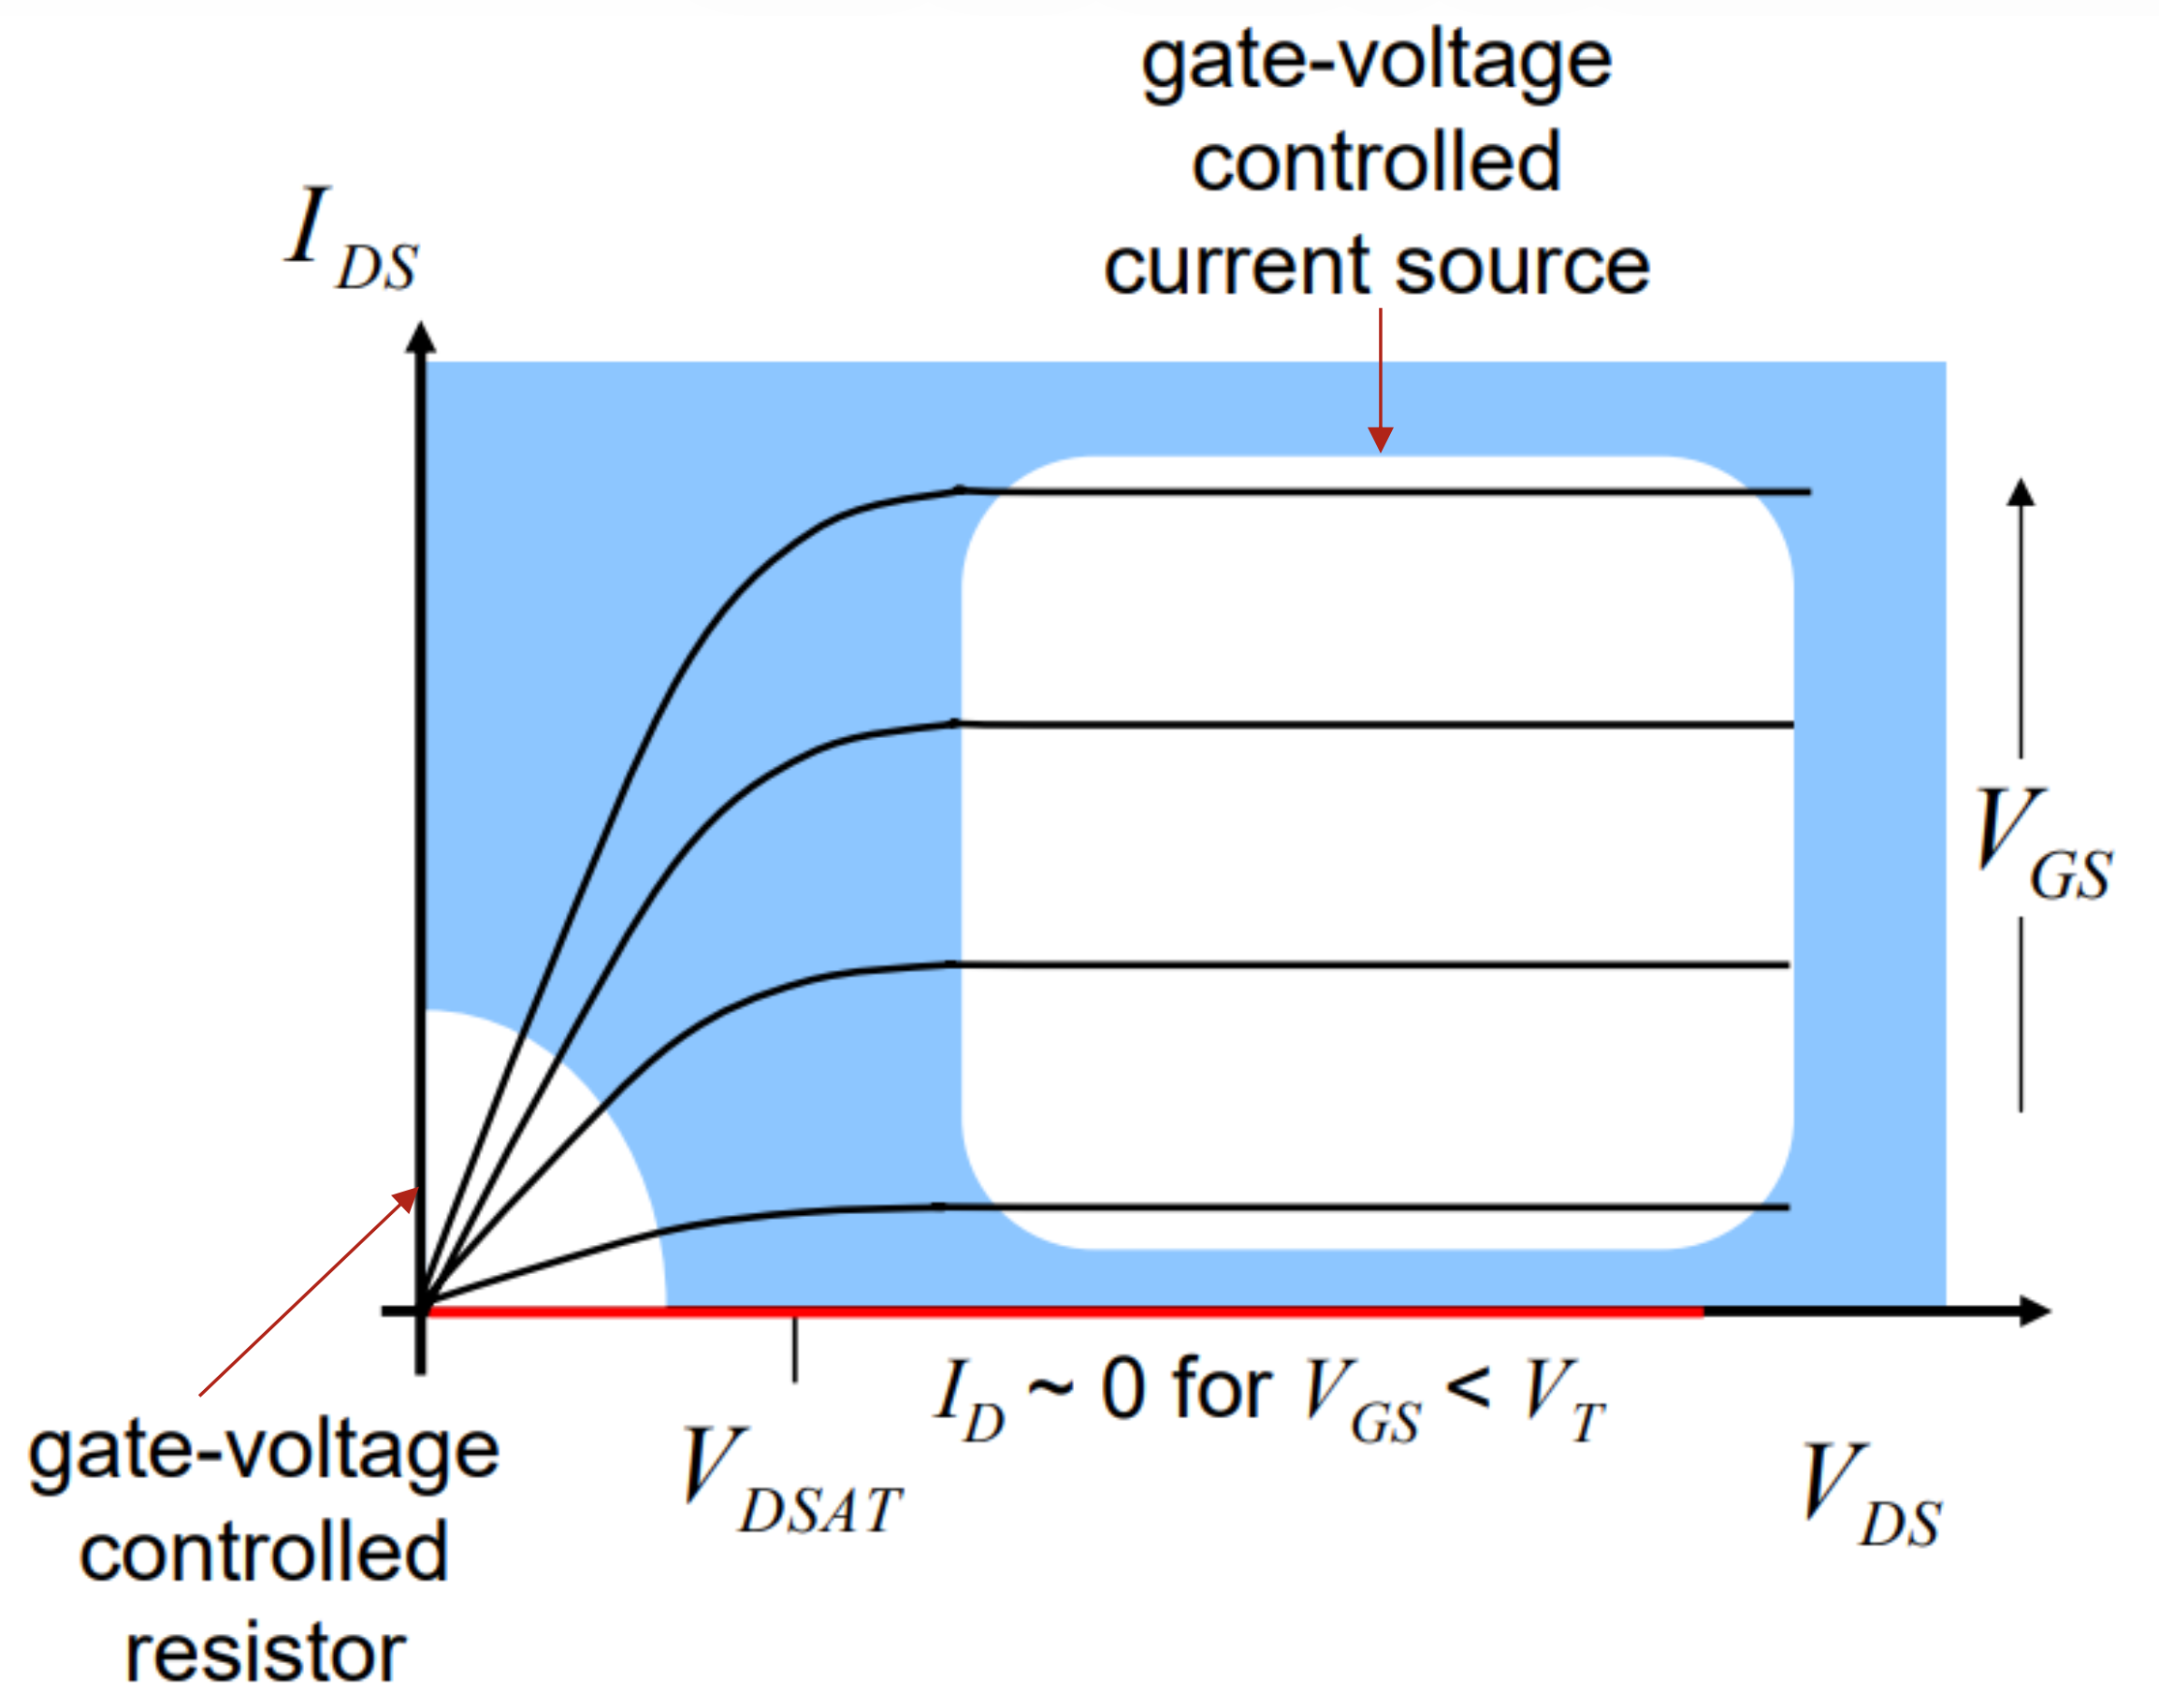
\includegraphics[width=0.5\textwidth]{immagini/nmos_characteristics.png}
\end{center}

\subsection{BJT}
\subsubsection*{Scheme}
A BJT (Bipolar Junction Transistor) is a three-terminal semiconductor device that can be used as a switch or as a current amplifier.
It is made of three layers of semiconductor material: the emitter (E), the base (B) and the collector (C). The current flowing from
collector to emitter (\(I_{CE}\)) is controlled by the current flowing into the base (\(I_B\)).

\begin{center}
	\begin{minipage}{0.45\textwidth}
		\centering 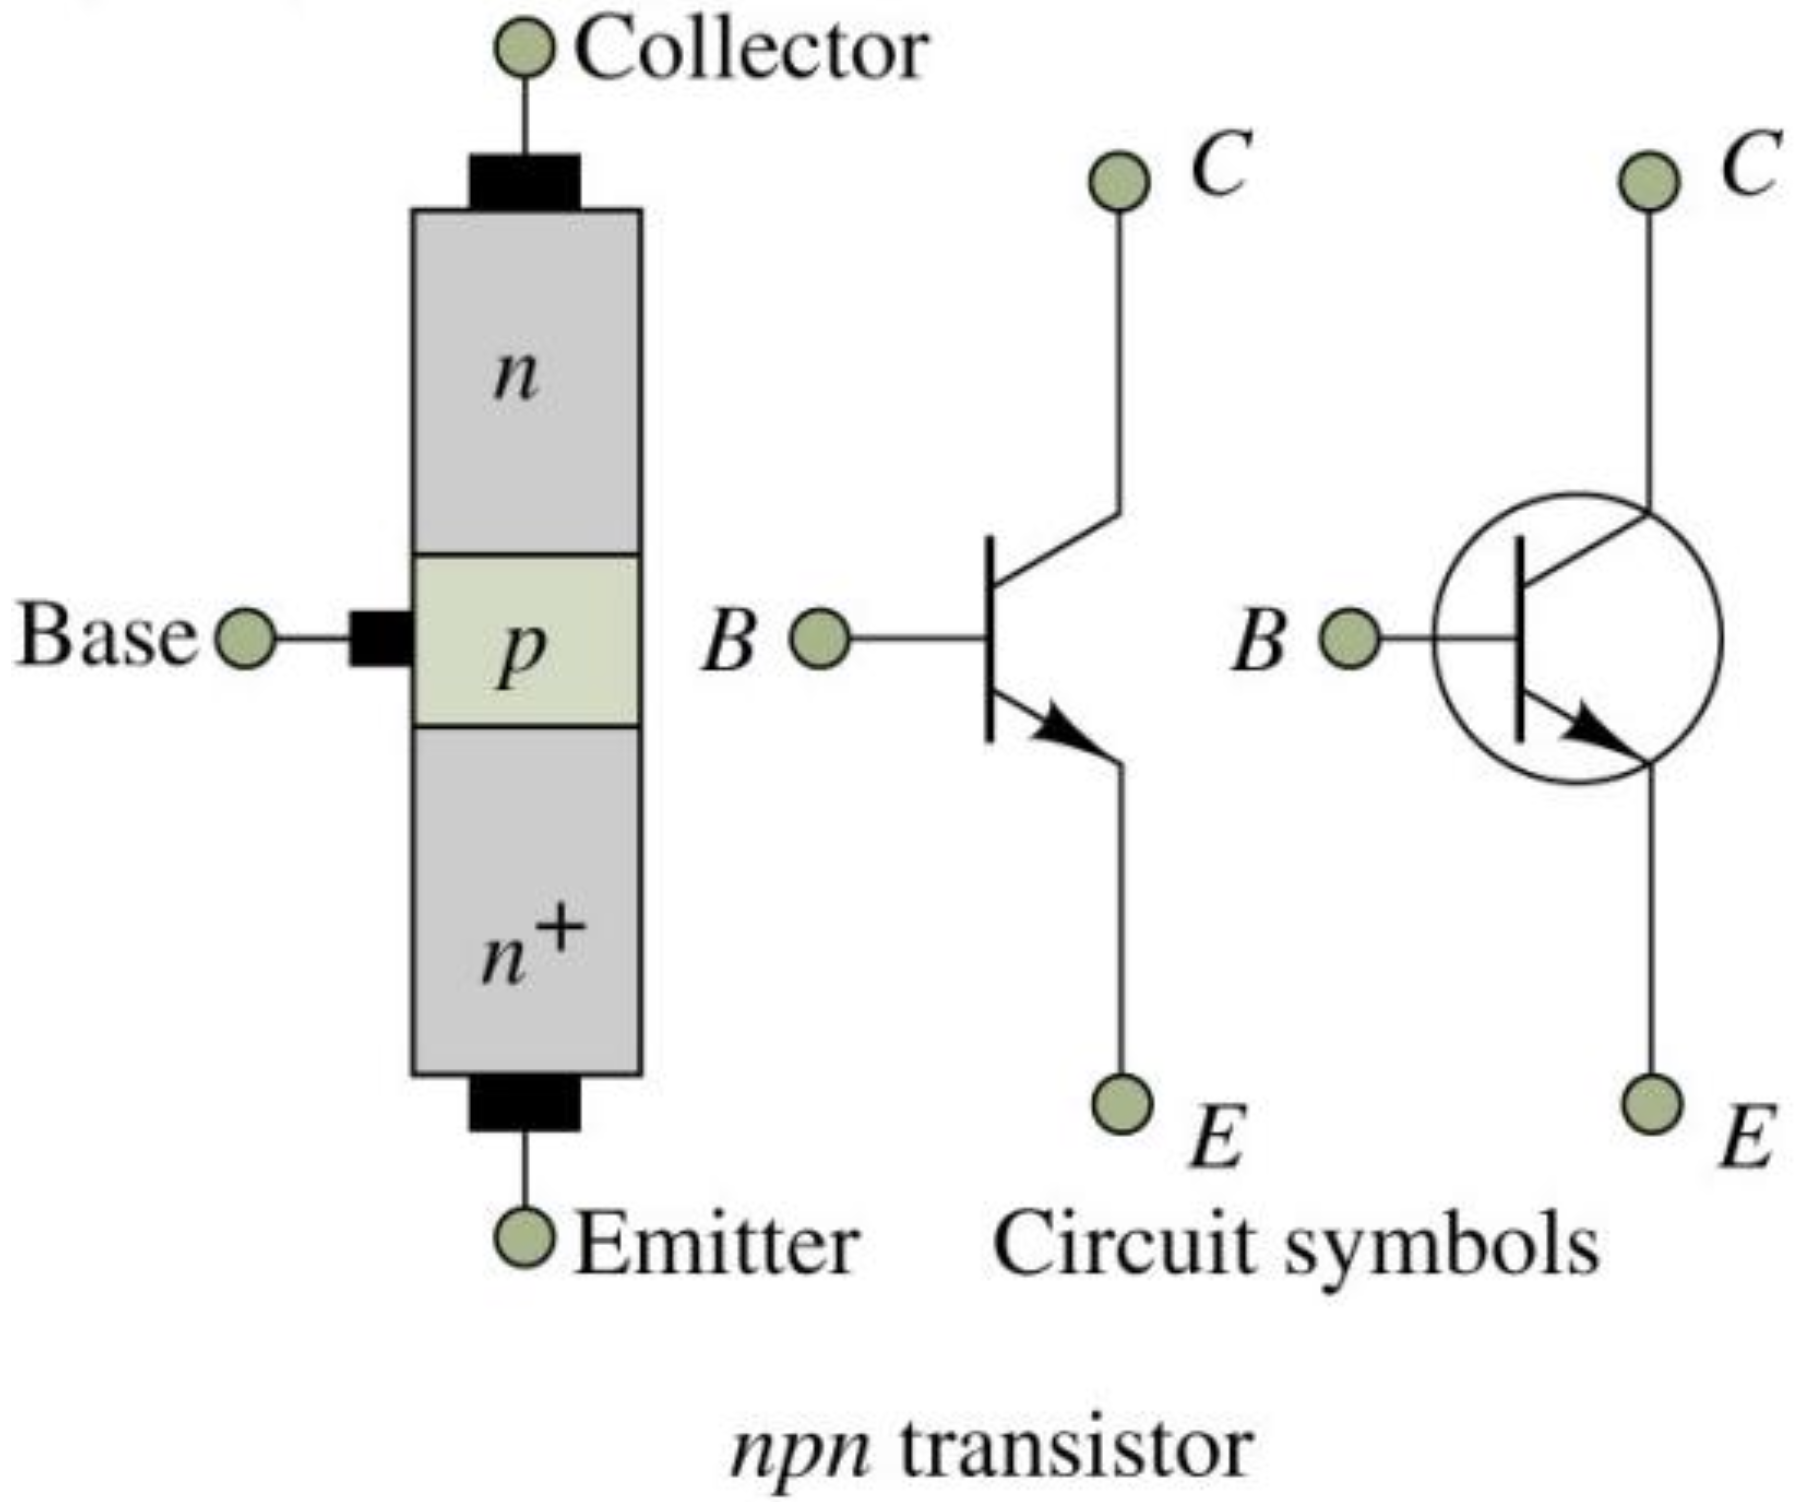
\includegraphics[width=0.8\textwidth]{immagini/npn_bjt.png}
	\end{minipage}
	\begin{minipage}{0.45\textwidth}
		\centering 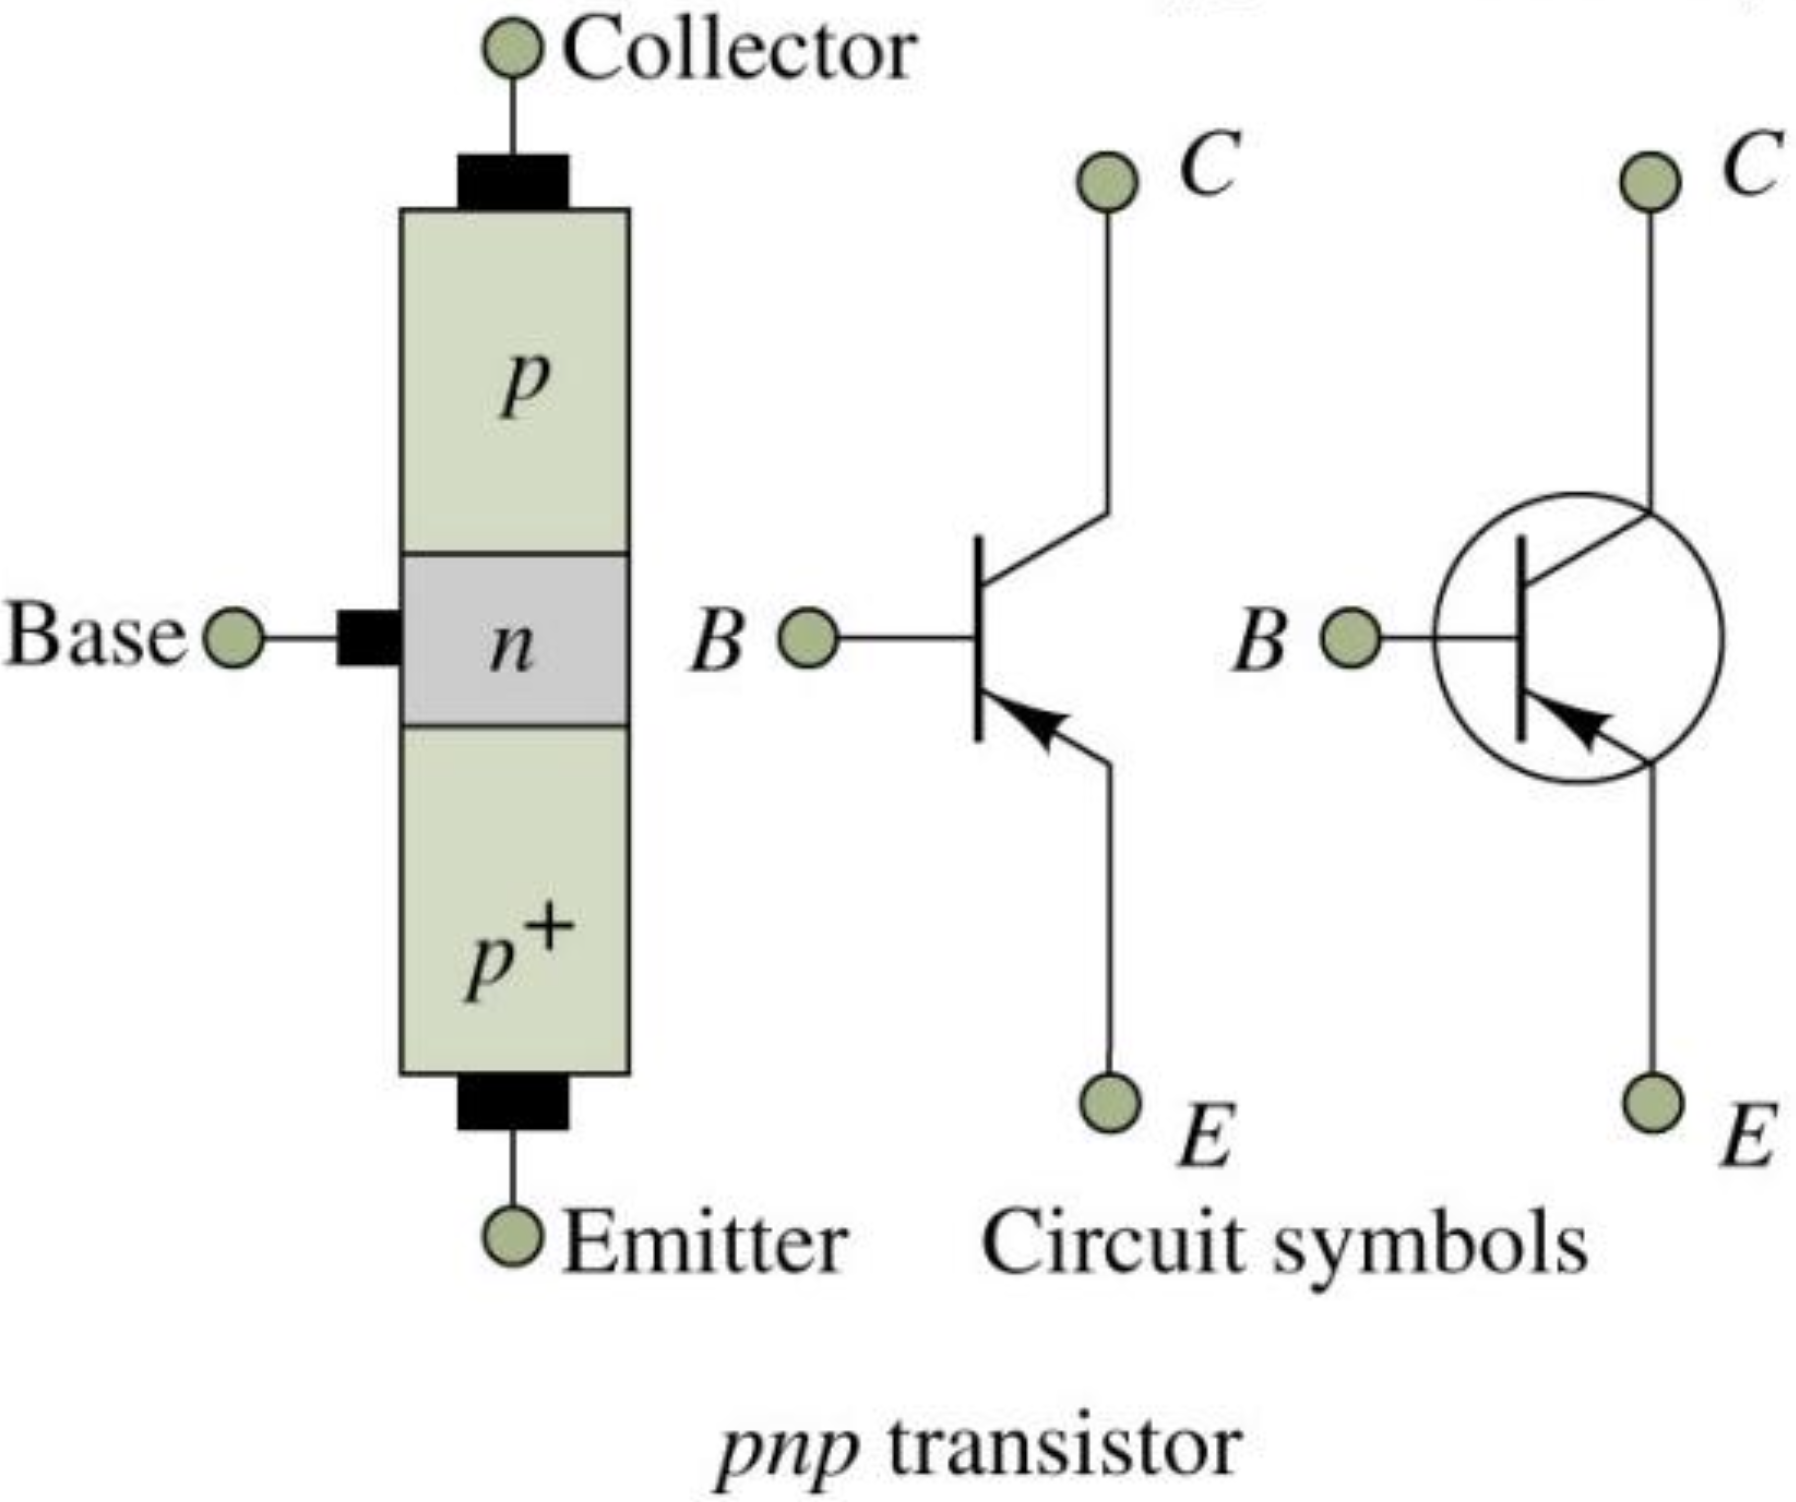
\includegraphics[width=0.8\textwidth]{immagini/pnp_bjt.png}
	\end{minipage}
\end{center}

\subsubsection*{Open Collector Curve}
When the base-emitter junction is forward biased and the collector is not connected to any voltage source (open collector), the BJT
behaves like a diode between the base and the emitter, with a voltage drop of about 0.7 V for silicon BJTs. There is an exponential
dependence between the base current \(I_B\) and the collector-emitter voltage \(V_{CE}\) (the same characteristic of a diode).
\[I_B = I_S \left(\exp \left( \frac{V_{BE}}{\eta V_T}\right) - 1\right)\]

\subsubsection*{Operation regions of a NPN BJT}
\begin{itemize}
	\item \textbf{forward active region} - \(V_C > V_B > V_E\): \\
	the BJT is a current amplifier, the collector current \(I_C\) is proportional to the base current \(I_B\) by a factor \(\beta\)
	and the emitter current \(I_E\) is the sum of the collector and base currents; the collector-base junction is reverse biased
	and the base-emitter junction is forward biased:
	\[I_C = \beta I_B \qquad\qquad I_E = I_C + I_B = (\beta + 1) I_B \qquad\qquad I_B = I_S \left(\exp \left( \frac{V_{BE}}{\eta V_T}\right) - 1\right)\]
	\item \textbf{saturation region} - \(V_C < V_B\) and \(V_E < V_B\): \\
	the BJT acts as a closed switch between the collector and emitter and both the collector-base and base-emitter junctions are
	forward biased; the collector current \(I_C\) depends only on the external circuit and previous equations are not valid anymore;
	the voltage drops \(V_{BE}\) and \(V_{CE}\) are approximately constant:
	\[V_{BE} \approx 0.7 \; V \qquad\qquad V_{CE} \approx V_{CE, sat} \approx 0.2 \; V\]
\end{itemize}

\section{OP AMPS - performance and limitations}
\subsection{Introduction}
OP amps (Operational Amplifiers) are high-gain voltage amplifiers with differential inputs and a single-ended output. In ideal
conditions, an OP amp has infinite gain, infinite input impedance, zero output impedance and infinite bandwidth, but in real
conditions those properties are not achievable.

\subsubsection*{History}
\begin{itemize}
	\item \textbf{1953}: K2-W - first commercially available OP amp based on vacuum tubes
	\item \textbf{1947}: first transistor (germanium) at Bell Labs
	\item \textbf{1954}: first silicon transistor at Texas Instruments
	\item \textbf{1958}: first integrated circuit at Texas Instruments
	\item \textbf{1960s}: solid state op-amps
	\item \textbf{1968}: Fairchild invented the \(\mu{A741}\) (commercially available as LM741), still used today
\end{itemize}

\subsection{Ideal op amp common circuit configurations}
\subsubsection*{Circuit model of an ideal op amp}
\begin{center}
	\begin{minipage}{0.35\textwidth}
		\centering \begin{circuitikz}[american, scale=0.7, transform shape]
			
			% Disegna il triangolo esterno dell'amplificatore operazionale
			\draw[line width=1pt] (0, 2.2) -- (4, 0) -- (0, -2.2) -- cycle;
	
			% disegna i terminali di ingresso
			\draw (-0.5, 1) node[left] (vplus) {$V^+$} to[short, o-] ++(0.85, 0)
				to[R, l=$R_{\mathrm{in}}$] ++(0, -2)
				to[short, -o] ++(-0.85, 0) node[left] (vminus) {$V^-$};
	
			% disegna la tensione di ingresso
			\draw[-{Latex}]
				(vminus) to[out=-250, in=250] 
				node[midway, fill=white, inner sep=2pt] {$V_{in}$} 
				(vplus);
	
			% generatore di tensione e resistenza
			\draw (4.5, 0) node[right] (vout) {$V_{out}$}
				to[short, o-] ++(-1, 0)
				to[R, l_=$R_{out}$] ++(-1.8, 0)
				to[cV, name=cgen] ++(0, -1.2)
				to[short] ++(0, -0.2) node[ground] {};
			\node at (cgen) [xshift=0.9cm, yshift=-0.4cm, fill=white, inner sep=1pt] {\(A \! \cdot \! V_{in}\)}; 
			
			% pin di alimentazione
			\draw (1.2, 1.55) to[short, -o] ++(0, 0.7) node[above] {$V_{DD+}$};
			\draw (1.2, -1.55) to[short, -o] ++(0, -0.7) node[below] {$V_{SS-}$};
	
		\end{circuitikz}
	\end{minipage}
	\begin{minipage}{0.6\textwidth}
		\begin{itemize}
			\item \(A\): open-loop gain of the op amp
			\item \(R_{in}\): input resistance of the op amp
			\item \(R_{out}\): output resistance of the op amp
			\item \(V_{in}\): differential input voltage (\(V_{in} = V^+ - V^-\))
			\item \(V_{out}\): output voltage
			\item \(V_{DD+}\) and \(V_{SS-}\): power supply voltages for the op amp
		\end{itemize}
	\end{minipage}
\end{center}

\subsubsection*{Inverting amplifier}
\begin{center}
	\begin{minipage}{0.35\textwidth}
		\centering \begin{circuitikz}[american, scale=0.8, transform shape]
			\node[op amp] (opamp) at (0,0) {};
			\draw (opamp.+) to[short] ++(0,-0.5) node[ground] {};
			\draw (opamp.-) to[R, l_=$R_{in}$] ++(-2,0) 
				node[left] {$V_{in}$}
				to[short, o-] ++(0,0);
			
			\draw (opamp.-) to[short, *-] ++(0, 1) coordinate (fb_up)
				to[R, l=$R_{f}$] (fb_up -| opamp.out)
				to[short, -*] (opamp.out);

			\draw (opamp.out) to[short, -o] ++(0.5,0) node[right] {$V_{out}$};
		\end{circuitikz}
	\end{minipage}
	\begin{minipage}{0.63\textwidth}
		Differential input voltage \(V_{in} = V^- - V^+\) must be zero to have a finite output voltage. For this reason,
		\(V^- = V^+ = 0V\) and the inverting input is called a virtual ground potential node because it is at ground
		potential but not directly connected to ground.
		
		The resistor series \(R_{in}\) and \(R_f\) acts as a voltage divider and the output voltage \(V_{out}\) is proportional
		to the input voltage \(V_{in}\) by a factor \(-R_f / R_{in}\):
		\[V_{out} = -\frac{R_f}{R_{in}} V_{in} \qquad H(s) = \frac{V_{out}}{V_{in}} = -\frac{R_f}{R_{in}}\]

		The output signal is out of phase (inverted) with the input signal.
	\end{minipage}
\end{center}

\subsubsection*{Non-inverting amplifier}
\begin{center}
	\begin{minipage}{0.35\textwidth}
		\centering \begin{circuitikz}[american, scale=0.8, transform shape]
			\node[op amp] (opamp) at (0,0) {};
			\draw (opamp.+) to[short, -o] ++(0, 0) node[left] {\(V_{in}\)};
			\draw (opamp.-) to[R, l_=$R_{in}$] ++(-2,0) node[ground] {};
			\draw (opamp.out) to[short, -o] ++(0.5,0) node[right] {$V_{out}$};

			\draw (opamp.-) to[short, *-] ++(0, 1) coordinate (fb_up)
				to[R, l=$R_{f}$] (fb_up -| opamp.out)
				to[short, -*] (opamp.out);
		\end{circuitikz}
	\end{minipage}
	\begin{minipage}{0.63\textwidth}
		To have a finite output voltage and a zero input differential voltage, \(V^+ = V^-\).
		
		The resistor series \(R_{in}\) and \(R_f\) acts as a voltage divider and the output voltage \(V_{out}\)
		is proportional to the input voltage \(V_{in}\) by a factor \(1 + R_f / R_{in}\):
		\[V_{out} = \left(1 + \frac{R_f}{R_{in}}\right) V_{in} \qquad H(s) = \frac{V_{out}}{V_{in}} = 1 + \frac{R_f}{R_{in}}\]

		The output signal is in phase (non-inverted) with the input signal.
	\end{minipage}
\end{center}

\subsubsection*{Voltage follower - buffer}
\begin{center}
	\begin{minipage}{0.35\textwidth}
		\centering \begin{circuitikz}[american, scale=0.9, transform shape]
			\node[op amp, xscale=0.6, yscale=0.6] (opamp) at (0,0) {};
			\draw (opamp.+) to[short, -o] ++(0, 0) node[left] {\(V_{in}\)};
			\draw (opamp.out) to[short, -o] ++(0.5,0) node[right] {$V_{out}$};

			\draw (opamp.-) to[short] ++(0, 0.6) coordinate (fb_up)
				to[short] (fb_up -| opamp.out)
				to[short, -*] (opamp.out);
		\end{circuitikz}
	\end{minipage}
	\begin{minipage}{0.63\textwidth}
		The voltage follower is a specific configuration of the non-inverting amplifier with no input and feedback resistors.
		The output signal is ideally an exact copy of the input signal from the non inverting input.
	\end{minipage}
\end{center}

\subsection{Ideal assumptions}
\begin{itemize}
	\item \textbf{infinite open-loop gain} \(A \to \infty\): the output voltage \(V_{out}\) can be arbitrarily large for any
	non-zero input voltage \(V_{in}\)
	\item \textbf{infinite input resistance} \(R_{in} \to \infty\): no current flows into the input terminals (zero input-bias
	current \(I_B = 0\)) and consequently the difference between the two input-bias currents is zero (zero input-offset current
	\(I_{OS} = 0\))
	\item \textbf{zero input offset voltage}: the output voltage is zero when the input voltage is zero
	\item \textbf{infinite common-mode rejection ratio (CMRR)}: the output voltage is only affected by the difference between
	the input voltages \(V^+ - V^-\) and not by the common-mode voltage \((V^+ + V^-)/2\)
	\item \textbf{zero output resistance} \(R_{out} \to 0\): the output voltage \(V_{out}\) is not affected by the load connected
	\item \textbf{infinite output voltage range}: the output voltage \(V_{out}\) is not limited by the power supply voltages
	and the op amp does not saturate
	\item \textbf{power supply rejection}: the output voltage is not affected by power supply voltage variations
	\item \textbf{infinite output current}: the op amp can provide any amount of current to the load
	\item \textbf{infinite open-loop bandwidth}: any frequency can be amplified without attenuation
	\item \textbf{infinite slew rate}: the output voltage can change instantaneously in response to changes in the input differential voltage
\end{itemize}

\subsection{Non idealities of op amps}
\subsubsection*{Input offset voltage}
When both inputs are connected to ground, the output has a small offset voltage \(V_0\) that keeps the output at some DC voltage
level instead of 0 V. This output voltage can be measured by connecting the op amp as a voltage follower with the non inverting
input connected to ground.

It is possible to create a model that include this effect by adding an ideal voltage generator in series to one of the two inputs
to generates a fixed input-voltage offset \(V_{OS}\). The \(V_{OS}\) is the equivalent differential voltage that must be provided
to an ideal op amp to obtain the output voltage offset \(V_0\).

Some ICs have specific pins to add a potentiometer that can be used to compensate the input offset voltage.

\begin{center}
	\begin{minipage}{0.45\textwidth}
		\centering \begin{circuitikz}[american, scale=0.8, transform shape]
			\node[op amp] (opamp) at (0,0) {};
			\draw (opamp.+) to[V, l=$V_{\mathrm{OS}}$] ++(-1,0) to[short, -o] ++(-0.5, 0) node[left] {\(V_{in}\)};
			\draw (opamp.-) to[short] ++(-1.5,0) to[R, l_=$R_{in}$] ++(-2,0) node[ground] {};
			\draw (opamp.out) to[short, -o] ++(0.5,0) node[right] {$V_{out}$};

			\draw (opamp.-) to[short] ++(-1.5,0) to[short, *-] ++(0, 1) coordinate (fb_up)
				to[R, l=$R_{f}$] (fb_up -| opamp.out)
				to[short, -*] (opamp.out);
			
			\draw[color=red] (-2.4,1.1) -- ++(3.4,0) -- ++(0,-2.7) -- ++(-3.4,0) -- cycle;
		\end{circuitikz} \\[5pt]
		\footnotesize Ideal op amp with zero output offset voltage \(V_0\) with non-ideal input offset voltage \(V_{OS}\)
		correction highlighted in the red rectangle.
	\end{minipage}
	\hfill
	\begin{minipage}{0.27\textwidth}
		\vspace{18pt}
		\centering \begin{circuitikz}[american, scale=0.8, transform shape]
			\node[op amp] (opamp) at (0,0) {};
			\draw (opamp.+) to[short] ++(0, 0) node[ground] {};
			\draw (opamp.out) to[short, -o] ++(0.5,0) node[right] {$V_{out}$};

			\draw (opamp.-) to[short] ++(0, 0.8) coordinate (fb_up)
				to[short] (fb_up -| opamp.out)
				to[short, -*] (opamp.out);
		\end{circuitikz} \\[10pt]
		\footnotesize Voltage follower configuration in which the output voltage is equal to the input offset voltage \(V_{OS}\).
	\end{minipage}
	\hfill
	\begin{minipage}{0.25\textwidth}
		\centering \begin{circuitikz}[american, scale=0.8, transform shape]
			\node[op amp] (opamp) at (0,0) {};
			\draw (opamp.+) to[short, -o] ++(0,0) node[left] {$V^+$};
			\draw (opamp.-) to[short, -o] ++(0,0) node[left] {$V^-$};
			\draw (opamp.out) to[short, -o] ++(0,0) node[right] {$V_{out}$};
			
			\draw[scale=0.5, transform shape] (-0.9, 1.5) -- ++(0, 0.7) to[R] ++(2, 0) -- ++(0, -1.9);

			\draw[<-, >=stealth] (0, 1.25) -- (0, 1.8) node[above] {\(V_{CC}\) or \(V_{EE}\)};
		\end{circuitikz} \\[5pt]
		\footnotesize Potentiometer for input offset voltage compensation
	\end{minipage}
\end{center}

Numerical example: if a non-inverting amplifier with \(R_f = 99 \; k\Omega\) and \(R_{in} = 1.2 \; k\Omega\) has an input offset
voltage of \(\left|V_{OS}\right| \leq 3 \; mV\), the output offset voltage \(V_0\) is:
\[\left|V_0\right| = \left|V_{OS}\right| \cdot \left(1 + \frac{R_f}{R_{in}}\right) = 3 \; mV \cdot \left(1 + \frac{99 \; k\Omega}{1.2 \; k\Omega}\right) = 0.25 \; V \quad \longrightarrow \quad -0.25 \; V < V_0 < 0.25 \; V\]

\subsubsection*{Input bias and offset currents}
Due to finite input resistance, there are small input bias currents \(I_{B_+}\) and \(I_{B_-}\) that flow into the input terminals
of the op amp. This happens because the input terminals are connected to the base or gate of internal transistors (BJT or MOSFET)
that have a non-infinite resistance. The difference between the two input bias currents is called input offset current \(I_{OS}\).

It is possible to create a model that include this effect by adding two ideal current generators in parallel to the input terminals
to simulate the input bias currents \(I_{B_+}\) and \(I_{B_-}\).

These currents cause voltage drops across the resistors \(R_{in}\) and \(R_f\) and consequently generate a small input
voltage offsets that will be amplified to a considerable output voltage offset. To mitigate this effect, it is recommended to
add a compensation resistor \(R_{B}\) between the non-inverting input and ground with a value equal to the parallel of \(R_{in}\)
and \(R_f\). Using this value, the output voltage offset depends only by the input offset current \(I_{OS}\) that is usually
5-10 times smaller than the individual input bias currents \(I_{B_+}\) and \(I_{B_-}\).
\[V_{out} = V_{out,1} + V_{out,2} = I_{B_-} \cdot R_f - I_{B_+} \cdot R_{B} \cdot \left(1 + \frac{R_f}{R_{in}} \right) \qquad \text{using superposition}\]
\[\text{using} \;\; R_B = R_f \parallel R_{in} = \frac{R_{in} \cdot R_f}{R_{in} + R_f} \quad \rightarrow \quad V_{out} = - (I_{B_+} - I_{B_-}) \cdot R_f = -I_{OS} \cdot R_f\]

\begin{center}
	\begin{minipage}{0.55\textwidth}
		\centering \begin{circuitikz}[american, scale=0.8, transform shape]
			\node[op amp] (opamp) at (0,0) {};
			\draw (opamp.+) to[short, -o] ++(-1.3, 0) node[above] {\(V_{in}\)};
			\draw (opamp.-) to[short] ++(-3.5,0) to[R, l_=$R_{in}$] ++(-2,0) node[ground] {};
			\draw (opamp.out) to[short, -o] ++(0.5,0) node[right] {$V_{out}$};

			\draw (opamp.-) to[short] ++(-3.5,0) to[short, *-] ++(0, 1) coordinate (fb_up)
				to[R, l=$R_{f}$] (fb_up -| opamp.out)
				to[short, -*] (opamp.out);
			
			\draw ($(opamp.+)+(-0.1,0)$) to[isource, name=ibplus] ++(0,-1.5) ++(0,0.18) node[ground] {};
			\draw ($(opamp.+)+(-0.9,0)$) to[R, l_=$R_B$] ++(0,-1.5) ++(0,0.18) node[ground] {};

			\draw ($(opamp.-)+(-2.5,0)$) to[isource, name=ibminus] ++(0,-1.5) ++(0,0.35) node[ground] {};
			
			\node at (ibplus) [xshift=0.6cm, yshift=-0.5cm, inner sep=1pt] {\(I_{B_+}\)}; 
			\node at (ibminus) [xshift=-0.4cm, yshift=-0.5cm, inner sep=1pt] {\(I_{B_-}\)}; 

			\draw[color=red] (-4.5,1.1) -- ++(5.5,0) -- ++(0,-3.6) -- ++(-5.5,0) -- cycle;
		\end{circuitikz}
	\end{minipage}
	\begin{minipage}{0.4\textwidth}
		Op amp model with current generators representing input bias currents \(I_{B_+}\) and \(I_{B_-}\) and compensation resistor
		\(R_B\) highlighted in the red rectangle.
	\end{minipage}
\end{center}

\subsubsection*{Input bias currents in integrators}
An integrator is a circuit configuration that integrates an input signal by storing charge on a capacitor \(C\) in the
feedback loop. The output voltage is proportional to the integral of the input signal. The capacitor has a normally open
switch in parallel to discharge the capacitor and reset the output voltage to the initial value.

\begin{center}
	\begin{minipage}{0.4\textwidth}
		\centering \begin{circuitikz}[american, scale=0.8, transform shape]
			\node[op amp] (opamp) at (0,0) {};
	
			\draw (opamp.out) to[short, -o] ++(0.5,0) node[right] {$V_{out}$};

			\draw (opamp.-) to[short] ++(-1,0) to[short, *-] ++(0, 1.3) coordinate (fb_up)
				to[C, name=c] (fb_up -| opamp.out)
				to[short, -*] (opamp.out);
			\node at (c) [xshift=0.4cm, yshift=-0.3cm, inner sep=1pt] {\(C\)}; 
			
			\draw (opamp.-) to[short] ++(-1,0) to[short, *-] ++(0, 2) coordinate (fb_up2)
				to[switch] (fb_up2 -| opamp.out)
				to[short] (opamp.out);
			
			\draw (opamp.+) -- ++(-0.2,0) to[vsource, name=ibplus] ++(0,-1.5) ++(0,0.35) node[ground] {};
			\draw (opamp.-) -- ++(-1.7,0) to[isource, l=\(I_{B_-}\)] ++(0,-1.5) ++(0,0.18) node[ground] {};
			\draw (opamp.-) -- ++(-2.5,0) to[R, l_=$R$] ++(0,-1.5) ++(0,0.18) node[ground] {}; 
			\node at (ibplus) [xshift=0.75cm, yshift=-0.4cm, inner sep=1pt] {\(V_{OS}\)};
			%\node at (ibminus) [xshift=-0.4cm, yshift=-0.5cm, inner sep=1pt] {\(I_{B_-}\)};
		\end{circuitikz}
	\end{minipage}
	\begin{minipage}{0.55\textwidth}
		NOTES:
		\begin{itemize}
			\item \(V_{OS}\) models the input offset voltage of real op amps
			\item \(I_{B_-}\) models the input bias current of real op amps
			\item useful formulas: \(V_C = Q_C / C\), \(\;\; Q_C = I_C \cdot t\)
		\end{itemize}
	\end{minipage}
\end{center}

\noindent
Analyzing the circuit behavior in the two possible states of the switch:
\begin{itemize}
	\item[1.] when the switch is closed, op amp acts as a voltage follower and \(V_{out} = V_{OS}\)
	\item[2.] when the switch is open, the output voltage \(V_{out}\) is:
	\[V_{out}(t) = V_{start} + V_{out,1} + V_{out,2} = V_{OS} + \frac{V_{OS}}{RC} t + \frac{I_{B}}{C} t\]
	\begin{itemize}[topsep=0pt]
		\item the input offset voltage \(V_{OS}\) that generates a current \(I_{OS} = V_{OS} / R\) through the resistor \(R\)
		that charge the capacitor \(C\) with a voltage contribution \(V_{out,1} = t \cdot V_{OS} / RC \)
		\item the input bias current \(I_{B}\) charge the capacitor \(C\) with a voltage contribution \(V_{out,2} = t \cdot I_{B} / C\)
		\item output voltage increases linearly with time and the slope is \(V_{OS} / RC + I_B / C\)
	\end{itemize}
\end{itemize}

\subsubsection*{Output voltage swing}
The output voltage swing is the range of output voltage that an op amp can provide without saturating. It is limited by 1-2 volts
below the power supply span. The saturation voltages \(L_+\) and \(L_-\) are asymmetrical and depend on the load connected to the
output and on the output current.

\subsubsection*{Output current limits}
The output current of an op amp is limited by short-circuit and power dissipation protection inside the op amp.

Sometimes datasheets specify only the output swing based on the load resistance \(R_L\), but not the maximum output current
\(I_{out, max}\). That value can be estimated by the following formula:
\[I_{out, max} = \frac{V_{out, max}}{R_L}\]

The output current is given by the sum of the load current \(I_L\) and the feedback current \(I_f\). Usually \(R_f\) is much larger
than \(R_L\) and the feedback current \(I_f\) is negligible compared to the load current \(I_L\). In general, for an inverting
amplifier the total output current \(I_{out}\) is:
\[I_{out} = I_L + I_f = \frac{V_{out}}{R_L} + \frac{V_{out}}{R_f + R_{in}} = V_{out} / R_{eq} \qquad \text{with} \quad R_{eq} = R_L \parallel (R_f + R_{in})\]

\begin{center}
	\begin{circuitikz}[american, scale=0.8, transform shape]
		\node[op amp] (opamp) at (0,0) {};
		\draw (opamp.+) to[short, -o] ++(0, 0) node[left] {\(V_{in}\)};
		\draw (opamp.-) to[R, l_=$R_{in}$] ++(-2,0) node[ground] {};
		\draw (opamp.out) -- ++(1, 0) to[R, l=$R_L$, i>^=$I_L$] ++(3,0) node[ground] {};
		\draw (opamp.out) ++(-0.3, 0) to[short, i=$I_{out}$] ++(0.7, 0);

		\draw (opamp.-) to[short, *-] ++(0, 1) coordinate (fb_up)
			to[R, l=$R_{f}$, ] (fb_up -| opamp.out)
			to[short] ++(0.7, 0) coordinate (fb_out)
			to[short, -*, i<=$I_f$] (fb_out |- opamp.out)
			to[short, -o] ++(0,-0.5) node[right] {\(V_{out}\)};
	\end{circuitikz}
\end{center}

\noindent
To correctly design the circuit and choose the correct feedback resistor \(R_f\) and input resistor \(R_{in}\) of an inverting
amplifier based on the load resistance \(R_L\), the following steps can be followed:
\begin{itemize}
	\item[1.] calculate the minimum equivalent resistance \(R_{eq} = R_L \parallel R_f\) based on \(V_{out, max}\) and \(I_{out, max}\)
	\item[2.] fix the load resistance based on the application requirements and calculate the minimum feedback resistor \(R_f\)
	(it is recommended to choose \(R_f\) slightly bigger than the minimum value)
	\item[3.] choose the input resistor \(R_{in}\) based on the desired gain of the amplifier and the value of \(R_f\) chosen
	in the previous step
	\item[4.] calculate the maximum output current \(I_{out}\) for the chosen resistor values and verify the requirements
\end{itemize}
It is recommended to choose resistor values between input impedance (\(1 \; M\Omega \; - \; 10 \; M\Omega\)) and output impedance
(\(10 \; \Omega \; - \; 100 \; \Omega\)) of the op amp. Usually, \(1 \; k\Omega \; - \; 100 \; k\Omega\) should be a good choice.

\subsubsection*{Slew rate and full-power bandwidth}
Slew rate is the maximum velocity with which the output voltage can change in response to a step input voltage. It is measured
in volts per microsecond (V/µs), usually in range \(0.1 \; V/\mu s \; - \; 10 \; V/\mu s\). If the input slew rate is higher than the op amp slew rate, the output will be clipped, filtered
or distorted.

The full-power bandwidth is the highest frequency at which a full-scale signal can be developed at the output without distortion.
It is related to the slew rate \(SR\) and the maximum output voltage \(V_{out, max}\) by the following formula:
\[f_{FPBW} = \frac{SR}{2 \pi \, V_{out, max}}\]
\[\text{\footnotesize sinusoidal output signal: } V_{out} = V_M \sin (\omega t) \quad \rightarrow \quad \text{\footnotesize signal slew rate: } \left. \frac{d V_{out}}{d t} \right|_{max} = \left. V_M \omega \cos (\omega t) \right|_{max} = V_M \omega\]
\[\text{\footnotesize signal SR should be less than the op amp SR: } \quad V_M \omega < SR \quad \rightarrow \quad V_M < \frac{SR}{\omega}\]
\[\text{\footnotesize obtaining the full-power bandwidth: } \quad \omega = 2 \pi f_M < \frac{SR}{V_M} \quad \rightarrow \quad f_M < \frac{SR}{2 \pi V_M}\]

\section{Linear voltage regulators}
\subsection{Performance indicators}
\subsubsection*{Line regulation}
Line regulation is the measure of how well a power supply maintains a constant output voltage \(V_{out}\) for a change in the
input voltage \(V_{in}\). It is usually expressed in percentage as the ratio of the change in output voltage to the change in
input voltage:
\[\text{Line regulation} = \frac{\Delta V_{out}}{\Delta V_{in}} \cdot 100\%\]

\subsubsection*{Load regulation}
Load regulation is the measure of how well a power supply maintains a constant output voltage \(V_{out}\) for a change in the load
conditions. It is usually expressed in percentage as the ratio between the maximum change in output voltage to the nominal output
voltage:
\[\text{Load regulation} = \frac{V_{out, min \; load} - V_{out, max \; load}}{V_{out, nominal \; load}} \cdot 100\%\]

\subsection{Simple Zener regulator}
\subsubsection*{Zener diode characteristic}
A Zener diode is a special type of diode that can operate in breakdown region (or Zener region) without being damaged. In reverse
breakdown region, the Zener diode maintains a constant voltage \(V_Z\) across its terminals for a wide range of current \(I_Z\)
between \(I_{Z,min}\) and \(I_{Z,max}\).

\subsubsection*{Simple Zener regulator}
The main idea of the simple Zener regulator is to use a Zener diode in reverse bias to maintain a constant output voltage
\(V_{out} = V_Z\) across the load. The input voltage \(V_{in}\) is connected to the series combination of a resistor \(R\)
and the Zener diode, and the load is connected in parallel to the Zener diode.
\begin{center}
	\begin{circuitikz}[american, scale=0.8, transform shape]
		\ctikzset{diodes/scale=0.8}
		\draw (0,1) node (vinplus) {} node[below] {\(+\)} to[short, o-] ++(0,0)
			to[R, l=$R_S$, i=$I_{RS}$] ++(3,0)
			to[short, i=$I_L$] ++(2.5,0) node (voutplus) {} node[right] {\(+\)}
			to[R, l_=$R_L$] ++(0,-2) node (voutminus) {} node[right] {\(-\)}
			to[short, -o] ++(-5.5,0) node (vinminus) {} node[above] {\(-\)};
		\draw (3.5,-1) node (vzenerminus) {} to[zzDo, i_<=$I_Z$] ++(0,2) node (vzenerplus) {};

		\node at (vzenerplus) [xshift=-0.3cm, yshift=-0.2cm] {\(+\)};
		\node at (vzenerminus) [xshift=-0.3cm, yshift=0.2cm] {\(-\)};

		\draw[-{Latex}]
			($(vinminus) + (-0.2, 0.1)$) to[out=120, in=240] 
			node[midway, fill=white, inner sep=4pt] {$V_{in}$} 
			($(vinplus) + (-0.2, -0.1)$);
		\draw[-{Latex}]
			($(voutminus) + (0.4, 0.1)$) to[out=60, in=-60] 
			node[midway, fill=white, inner sep=4pt] {$V_{out}$} 
			($(voutplus) + (0.4, -0.1)$);
		\draw[-{Latex}]
			($(vzenerminus) + (-0.5, 0.3)$) to[out=130, in=-130] 
			node[midway, fill=white, inner sep=2pt] {$V_Z$} 
			($(vzenerplus) + (-0.5, -0.3)$);
	\end{circuitikz}
\end{center}

\noindent
To ensure proper operation, component values must be chosen to satisfy the following conditions:
\begin{itemize}
	\item the series resistor \(R_S\) must be large enough to limit the current through the Zener diode \(I_Z < I_{Z,max}\) when
	load is disconnected and all the current flows through the Zener diode:
	\[R_S \geq \frac{V_{in} - V_Z}{I_{Z,max}}\]
	\item the load resistor \(R_L\) must be large enough to ensure the minimum Zener diode current \(I_Z > I_{Z,min}\); if the
	load is too small, current will flow only through the load and the Zener diode will not be able to maintain a constant
	output voltage:
	\[R_L \geq \frac{V_Z}{I_{RS} - I_{Z,min}}\]
\end{itemize}

\subsubsection*{Limitations of the simple Zener regulator}
\begin{itemize}
	\item Due to constant voltage \(V_{RS}\) and constant current \(I_{RS}\), there is a constant and significant power dissipation
	in the series resistor \(R_S\) even when the load is disconnected, especially when the load can require a large current \(I_L\).
	\item Output voltage \(V_{out}\) changes linearly with variation of the load current \(I_L\) due to the not null Zener impedance
	\(R_Z\): \(V_{out} = V_Z + I_Z R_Z\), this circuit has poor load regulation.
\end{itemize}

\subsection{Transistor series voltage regulator}
\subsubsection*{Circuit}
The main idea is to use a transistor \(Q_1\) as a variable resistor in series with the load, and to use a Zener diode to maintain
a constant voltage \(V_Z\) at the base of the transistor. The output voltage \(V_{out}\) is constant and equal to the difference
between the Zener voltage \(V_Z\) (constant) and the base-emitter voltage \(V_{BE}\) (also approximately constant):
\[V_{out} = V_Z - V_{BE}\]

\noindent
The series resistor \(R_S\) is used to guarantee that the current through the Zener diode respects the datasheet specifications
\(I_{Z,max} > I_Z > I_{Z,min}\):
\[\frac{V_{in} - V_Z}{I_{Z,min} + I_B} \; > \; R_S \; > \; \frac{V_{in} - V_Z}{I_{Z,max} + I_B} \qquad\qquad \text{where} \; I_B = \frac{I_L}{\beta} = I_S \cdot \left(e^{\frac{V_{BE}}{\eta V_T}} - 1\right)\]

\begin{center}
	\begin{minipage}{0.8\textwidth}
		\centering \begin{circuitikz}[scale=0.8, transform shape]
			\ctikzset{diodes/scale=0.8}
			\node[npn, rotate=90] (Q1) at (3,4) {};
			\node[above] at (3, 4) {$Q_1$};
			\draw (0, 4) node[circ] (vinplus) {} node[below] {\(+\)} -- (Q1.C);
			\draw (0, 0) node[circ] (vinminus) {} node[above] {\(-\)} -- (6, 0);
			\draw (1.5, 4) to[R, l_=$R_S$] (1.5, 2) to[short, i=$I_{RS}$] (3, 2) to[short, i_=$I_B$] (Q1.B);
			\draw (3, 0) node(vzenerminus) {} to[zzDo, i_<=$I_Z$] (3, 2) node(vzenerplus) {};
			\draw (Q1.E) to[short, i_=$I_L$] (6, 4) node[circ] (voutplus) {} node[right] {\(+\)} to[R, l_=$R_L$] (6, 0) node[circ] (voutminus) {} node[right] {\(-\)};
	
			\node at (vzenerplus) [xshift=-0.3cm, yshift=-0.2cm] {\(+\)};
			\node at (vzenerminus) [xshift=-0.3cm, yshift=0.2cm] {\(-\)};
	
			\node at (Q1.B) [xshift=0.2cm, yshift=-0.1cm] (q1b) {\(+\)};
			\node at (Q1.E) [xshift=0.2cm, yshift=-0.2cm] (q1e) {\(-\)};
	
			\draw[-{Latex}]
				($(vinminus) + (-0.2, 0.1)$) to[out=120, in=-120] 
				node[midway, fill=white, inner sep=4pt] {$V_{in}$} 
				($(vinplus) + (-0.2, -0.1)$);
			\draw[-{Latex}]
				($(voutminus) + (0.5, 0.1)$) to[out=60, in=-60] 
				node[midway, fill=white, inner sep=4pt] {$V_{out}$} 
				($(voutplus) + (0.5, -0.1)$);
			\draw[-{Latex}]
				($(vzenerminus) + (-0.5, 0.3)$) to[out=130, in=-130] 
				node[midway, fill=white, inner sep=2pt] {$V_Z$} 
				($(vzenerplus) + (-0.5, -0.3)$);
			\draw[-{Latex}]
				($(q1e) + (0, -0.1)$) to[out=260, in=0] 
				node[pos=0.35, fill=white, inner sep=1pt] {$V_{BE}$} 
				($(q1b) + (0.2, 0)$);
		\end{circuitikz}
	\end{minipage}
\end{center}

\subsubsection*{Advantages compared to the simple Zener regulator}
\begin{itemize}
	\item the circuit is more resilient to variations in the load current \(I_L\) because when the transistor works in forward
	active region, a change in the emitter current \(I_L = I_E\) produces mainly a change in the collector current \(I_C\) and
	only a small change in the base current \(I_B = I_C / \beta\), so the Zener diode current \(I_Z\) remains almost constant
	\item there is also a feedback effect: if the \(V_L\) drops, \(V_{BE}\) increases, the transistor \(Q_1\) becomes more
	conductive and \(V_{out}\) increases again; vice versa if \(V_{out}\) increases
	\item the power dissipation in the series resistor \(R_S\) is reduced because the current through it doesn't have to be
	large enough to power the load \(I_L\) but only to guarantee the minimum Zener current \(I_Z\)
\end{itemize}

\subsubsection*{Problems and limitations}
\begin{itemize}
	\item with circuit heating, \(V_Z\) and \(V_{BE}\) can change in different ways, so the output voltage \(V_{out}\) is
	subject to temperature variations
	\item the output voltage \(V_{out}\) can't be controlled or adjusted to a specific value, it is fixed by the Zener voltage
	\(V_Z\) and the base-emitter voltage \(V_{BE}\)
\end{itemize}

\newpage

\subsection{Adjustable series voltage regulator with feedback}
\subsubsection*{Circuit}
The idea of the circuit is to use the transistor series voltage regulator (described in the previous section) to impose
a constant voltage \(V_F\) to the partial resistor \(R_2\) of the potentiometer that acts as a voltage divider made of
two resistors \(R_1\) and \(R_2\). The output voltage \(V_{out}\) is given by:
\[V_{out} = I_{R2} \cdot (R_1 + R_2) = \frac{V_F}{R_2} \cdot (R_1 + R_2) = \frac{V_Z + V_{BE1}}{R_2} (R_1 + R_2)\]

\noindent
The transistor \(Q_2\) is used as a pass transistor to provide the required current to the load.

\begin{center}
	\begin{minipage}{0.9\textwidth}
		\centering 
		\begin{circuitikz}[scale=0.8, transform shape]
			\ctikzset{diodes/scale=0.8}
			% Q2: Transistor di potenza superiore
			% rotate=90 ruota il BJT NPN in modo che il collettore sia a sinistra e l'emettitore a destra
			\node[npn, rotate=90] (Q2) at (4, 5) {};
			\node[above] at (4, 5) {$Q_2$};

			% Q1: Transistor amplificatore di errore
			% xscale=-1 inverte orizzontalmente il transistor mettendo la base a destra
			\node[npn, xscale=-1] (Q1) at (4, 2.8) {};
			\node[left=20pt] at (Q1.B) {$Q_1$};

			% Terminali di ingresso e linee principali (Top e Bottom Rails)
			\draw (0, 5) node[circ] (vinplus) {} node[below] {\(+\)} -- (Q2.C);
			\draw (0, 0) node[circ] (vinminus) {} node[above] {\(-\)} -- (8.5, 0);

			% Ramo della resistenza Rs
			\draw (1.5, 5) node {} to[R, l_=$R_S$] (1.5, 2) -- (Q1.E);

			% Ramo della resistenza R3
			\draw (2.5, 5) node {} to[R, l_=$R_3$] (2.5, 3.5) to[short] (4, 3.5);

			% Connessione tra Collettore di Q1 e Base di Q2
			\draw (Q1.C) -- (Q2.B);

			% Diodo Zener
			\draw (4, 0) node (vzenerminus) {} to[zzDo] (4, 2) node (vzenerplus) {} -- ++(0,0.5);

			% Ramo di Uscita e Carico RL
			\draw (Q2.E) -- (8.5, 5) node[circ] (voutplus) {} node[right] {\(+\)};
			\draw (8.5, 0) node[circ] (voutminus) {} node[right] {\(-\)};
			\draw (8.5, 5) to[R, l_=$R_L$] (8.5, 0);

			% Partitore di tensione (R1 e R2)
			\draw (6.5, 5) node {} to[R] (6.5, 0.5) -- ++(0, -0.5);

			\draw[{Latex}-{Latex}] (7, 5) to[] node[midway, fill=white, inner sep=1pt] {$R_1$} (7, 2.7);
			\draw[{Latex}-{Latex}] (7, 2.7) to[] node[midway, fill=white, inner sep=1pt] {$R_2$} (7, 0);

			% Cursore K (collegamento alla base di Q1)
			\draw[-{Latex}] (Q1.B) -- ++(1.5, 0) node[pos=0.8, above] {K} node[below, xshift=-0.3cm, yshift=-0.1cm] (vfplus) {\(+\)};
			\node at (vfplus) [xshift=0.1cm, yshift=-2.2cm] (vfminus) {\(-\)};

			% Etichette di polarità (+ / -) interne
			\node at (vzenerplus) [xshift=-0.4cm, yshift=-0.2cm] {\(+\)};
			\node at (vzenerminus) [xshift=-0.4cm, yshift=0.2cm] {\(-\)};

			% Posizionamento dei nodi per l'arco V_BE1
			\node at ($(Q1.B) + (0.2, -0.2)$) (q1b) {\(+\)};
			\node at ($(Q1.E) + (0.2, -0.2)$) (q1e) {\(-\)};

			\node at (Q2.B) [xshift=0.2cm, yshift=-0.1cm] (q2b) {\(+\)};
			\node at (Q2.E) [xshift=0.2cm, yshift=-0.2cm] (q2e) {\(-\)};

			% Frecce delle tensioni (usando la tua struttura originaria)
			\draw[-{Latex}]
				($(vinminus) + (-0.2, 0.1)$) to[out=120, in=-120] 
				node[midway, fill=white, inner sep=4pt] {$V_{in}$} 
				($(vinplus) + (-0.2, -0.1)$);
				
			\draw[-{Latex}]
				($(voutminus) + (0.5, 0.1)$) to[out=60, in=-60] 
				node[midway, fill=white, inner sep=4pt] {$V_{out}$} 
				($(voutplus) + (0.5, -0.1)$);
				
			\draw[-{Latex}]
				($(vzenerminus) + (-0.5, 0.3)$) to[out=130, in=-130]
				node[midway, fill=white, inner sep=2pt] {$V_Z$} 
				($(vzenerplus) + (-0.5, -0.3)$);
				
			\draw[-{Latex}]
				($(q1e) + (0.2, 0)$) to[out=-20, in=-50] 
				node[pos=0.5, fill=white, inner sep=1pt] {$V_{BE1}$} 
				($(q1b) + (0.1, -0.1)$);
			
			\draw[-{Latex}]
				($(q2e) + (0, -0.1)$) to[out=260, in=0] 
				node[pos=0.35, fill=white, inner sep=1pt] {$V_{BE2}$} 
				($(q2b) + (0.2, 0)$);
			
			\draw[-{Latex}]
				($(vfminus) + (-0.1, 0.3)$) to[out=110, in=-110] 
				node[midway, fill=white, inner sep=1pt] {$V_F$} 
				($(vfplus) + (-0.1, -0.3)$);
		\end{circuitikz}
	\end{minipage}
\end{center}

\subsubsection*{Advantages compared to the transistor series voltage regulator}
\begin{itemize}
	\item the output voltage \(V_{out}\) can be adjusted by changing the ratio between the two half resistors \(R_1\) and \(R_2\)
	of the potentiometer in the voltage divider
	\item the feedback effect is more complex and stronger: if \(V_{out}\) increases, \(V_F\) increases, \(V_{BE1}\) increases, 
	\(I_{C1}\) increases, \(V_{R3}\) increases, \(V_{B2}\) decreases, \(V_{BE2}\) decreases, \(I_{E2}\) decreases, \(V_{out}\)
	decreases again; vice versa if \(V_{out}\) decreases
\end{itemize}

\subsection{Short circuit protection}
\subsubsection*{Circuit}
Short circuit protection is implemented by adding a transistor \(Q_3\) and a small resistor \(R_4\) (\(\approx 1 \; \Omega\)) in
the output branch (highlighted by the red rectangle in the circuit). When the load current \(I_L\) is too high, the voltage drop
across \(R_4\) becomes large enough to turn on the transistor \(Q_3\), which starts to absorb current from the resistor \(R_3\)
that produce a voltage drop \(V_{R3}\) that reduces the base voltage of \(Q_2\) and consequently the voltage \(V_{BE2}\) that
turns off \(Q_2\) and reduces the current \(I_L\) to a safe value.

The limit current \(I_{L,max}\) that can be delivered to the load is approximately given by:
\[I_{L,max} \approx \frac{V_{BE3, turn \, on}}{R_4}\]

\begin{center}
	\begin{minipage}{0.9\textwidth}
		\centering 
		\begin{circuitikz}[scale=0.8, transform shape]
			\ctikzset{diodes/scale=0.8}
			% Q2: Transistor di potenza superiore
			% rotate=90 ruota il BJT NPN in modo che il collettore sia a sinistra e l'emettitore a destra
			\node[npn, rotate=90] (Q2) at (3.5, 5) {};
			\node[above] at (3.5, 5) {$Q_2$};

			% Q1: Transistor amplificatore di errore
			% xscale=-1 inverte orizzontalmente il transistor mettendo la base a destra
			\node[npn, xscale=-1] (Q1) at (3.5, 2.2) {};
			\node[left=20pt] at (Q1.B) {$Q_1$};

			% Terminali di ingresso e linee principali (Top e Bottom Rails)
			\draw (0, 5) node[circ] (vinplus) {} node[below] {\(+\)} -- (Q2.C);
			\draw (0, 0) node[circ] (vinminus) {} node[above] {\(-\)} -- (8.5, 0);

			% Ramo della resistenza Rs
			\draw (1, 5) node {} to[R, l_=$R_S$] (1, 1.5) -- (Q1.E);

			% Ramo della resistenza R3
			\draw (2, 5) node {} to[R, l_=$R_3$] (2, 3.5) to[short] (3.5, 3.5) node[circ] {};

			% Q3: Transistor di protezione contro cortocircuiti
			\node[npn, rotate=90, xscale=-1, anchor=collector] (Q3) at (3.5, 3.5) {};
			\node[below=20pt] at (Q3.B) {$Q_3$};
			\draw (Q2.E) -- (Q3.B);
			\draw (Q3.E) -- ++(0.9, 0) -- ++(0, 1.5);

			% Connessione tra Collettore di Q1 e Base di Q2
			\draw (Q1.C) -- (Q2.B);

			% Diodo Zener
			\draw (3.5, 0) node (vzenerminus) {} to[zzDo] (3.5, 1.5) node (vzenerplus) {} -- ++(0,0.2);

			% Ramo di Uscita e Carico RL
			\draw (Q2.E) to[R, l_=$R_4$] ++(1.5, 0) -- (8.5, 5) node[circ] (voutplus) {} node[right] {\(+\)};
			\draw (8.5, 0) node[circ] (voutminus) {} node[right] {\(-\)};
			\draw (8.5, 5) to[R, l_=$R_L$] (8.5, 0);

			% Partitore di tensione (R1 e R2)
			\draw (6.5, 5) -- ++(0,-0.5) to[R] (6.5, 0) -- ++(0, -0);

			\draw[{Latex}-{Latex}] (7, 5) to[] node[midway, fill=white, inner sep=1pt] {$R_1$} (7, 2.2);
			\draw[{Latex}-{Latex}] (7, 2.2) to[] node[midway, fill=white, inner sep=1pt] {$R_2$} (7, 0);

			% Cursore K (collegamento alla base di Q1)
			\draw[-{Latex}] (Q1.B) -- ++(1.9, 0) node[pos=0.8, above] {K} node[below, xshift=-0.3cm, yshift=-0.1cm] (vfplus) {\(+\)};
			\node at (vfplus) [xshift=0.1cm, yshift=-1.7cm] (vfminus) {\(-\)};

			% Etichette di polarità (+ / -) interne
			\node at (vzenerplus) [xshift=-0.4cm, yshift=-0.2cm] {\(+\)};
			\node at (vzenerminus) [xshift=-0.4cm, yshift=0.2cm] {\(-\)};

			% Frecce delle tensioni (usando la tua struttura originaria)
			\draw[-{Latex}]
				($(vinminus) + (-0.2, 0.1)$) to[out=120, in=-120] 
				node[midway, fill=white, inner sep=4pt] {$V_{in}$} 
				($(vinplus) + (-0.2, -0.1)$);
				
			\draw[-{Latex}]
				($(voutminus) + (0.5, 0.1)$) to[out=60, in=-60] 
				node[midway, fill=white, inner sep=4pt] {$V_{out}$} 
				($(voutplus) + (0.5, -0.1)$);
				
			\draw[-{Latex}]
				($(vzenerminus) + (-0.5, 0.3)$) to[out=140, in=-140]
				node[midway, fill=white, inner sep=1pt] {$V_Z$} 
				($(vzenerplus) + (-0.5, -0.3)$);
			
			\draw[-{Latex}]
				($(vfminus) + (-0.1, 0.3)$) to[out=110, in=-110] 
				node[midway, fill=white, inner sep=1pt] {$V_F$} 
				($(vfplus) + (-0.1, -0.3)$);

			\draw[color=red] (1.25, 5.6) -- ++(5, 0) -- ++(0,-2.5) -- ++(-5,0) -- cycle;
		\end{circuitikz}
	\end{minipage}
\end{center}

\section{Signal generators}
\subsection{Bistable circuits - Schmitt trigger}
\subsubsection*{Generic bistable circuit - schmitt trigger}
A generic bistable circuit, called also schmitt trigger is a circuit that has two stable states and can remain in either state
indefinitely until an external trigger is applied to change its state. 

It can be made of an op amp with positive feedback (no virtual ground). When the circuit turns on, \(V_{out}\), \(V_+\) and
\(V_-\) are initially at \(0 \; V\). A slight variation in the input voltage \(V_+\) will cause the output to saturate at either
\(L_+\) or \(L_-\) depending on the sign of the variation. These two final states are the two stable states of the circuit.
Due to the positive feedback, the circuit will remain in the stable state until an external trigger is applied to one of the
input terminals.

\begin{center}
	\begin{circuitikz}[american, scale=0.8, transform shape]
		\draw (0,0) node[op amp, yscale=-1] (opamp) {};
		\node[ground] at (opamp.-) {}; 
		\node[left] at (opamp.+) {\(V_+\)};
		\draw (opamp.+) -- ++(0,1);
		\draw (opamp.out) to[short, -o] ++(0.5,0) node[right] {\(V_{out}\)};
		\draw (opamp.out) -- ++(0, 1.5)
			to[R, l=\(R_2\)] ++(-2.5, 0)
			to[R, l=\(R_1\)] ++(-2, 0) node[ground] {};
	\end{circuitikz}
\end{center}

\subsubsection*{Inverting bistable circuit}
An inverting bistable circuit is a Schmitt trigger with a voltage generator (that acts as a trigger) connected to the inverting
input of the op amp. It is called ``inverting'' because the output voltage is inverted with respect to the input trigger voltage. 

The output voltage \(V_{out}\) will be at \(L_+\) and \(V_+ = L_+ \cdot R_1 / (R_1 + R_2)\) until the input trigger voltage
\(V_{in}\) exceeds the positive threshold voltage \(V_{TH} = L_+ \cdot R_1 / (R_1 + R_2)\). In this case the differential input
voltage becomes negative (\(V_+ - V_{in} < 0\)), the output voltage \(V_{out}\) will switch to \(L_-\) and
\(V_+ = L_- \cdot R_1 / (R_1 + R_2)\).

To switch back to \(L_+\), the input trigger voltage \(V_{in}\) must be lower than the negative threshold voltage
\(V_{TL} = L_- \cdot R_1 / (R_1 + R_2)\). In this case the differential input voltage become positive again
(\(V_+ - V_{in} > 0\)) to switch the output back to \(L_+\).

\[V_{out} = L_+ \quad \Longleftrightarrow \quad V_+ - V_{in} = L_+ \cdot \frac{R_1}{R_1 + R_2} - V_{in} > 0 \quad \Longrightarrow \quad V_{in} < V_{TH} = L_+ \cdot \frac{R_1}{R_1 + R_2}\]
\[V_{out} = L_- \quad \Longleftrightarrow \quad V_+ - V_{in} = L_- \cdot \frac{R_1}{R_1 + R_2} - V_{in} < 0 \quad \Longrightarrow \quad V_{in} > V_{TL} = L_- \cdot \frac{R_1}{R_1 + R_2}\]

\begin{center}
	\begin{minipage}{0.45\textwidth}
		\centering \begin{circuitikz}[american, scale=0.8, transform shape]
			\draw (0,0) node[op amp, yscale=-1] (opamp) {};
			\node[left] at (opamp.+) {\(V_+\)};
			\draw (opamp.+) -- ++(0,1);
			\draw (opamp.out) to[short, -o] ++(0.5,0) node[right] {\(V_{out}\)};
			\draw (opamp.out) -- ++(0, 1.5)
			to[R, l=\(R_2\)] ++(-2.5, 0)
			to[R, l=\(R_1\)] ++(-2, 0) node[ground] {};
			\draw (opamp.-) -- ++(-0.5, 0) to[vsource, l_=\(V_{in}\)] ++(0, -1.5) ++(0, 0.3) node[ground] {};
		\end{circuitikz}
	\end{minipage}
	\begin{minipage}{0.45\textwidth}
		\centering 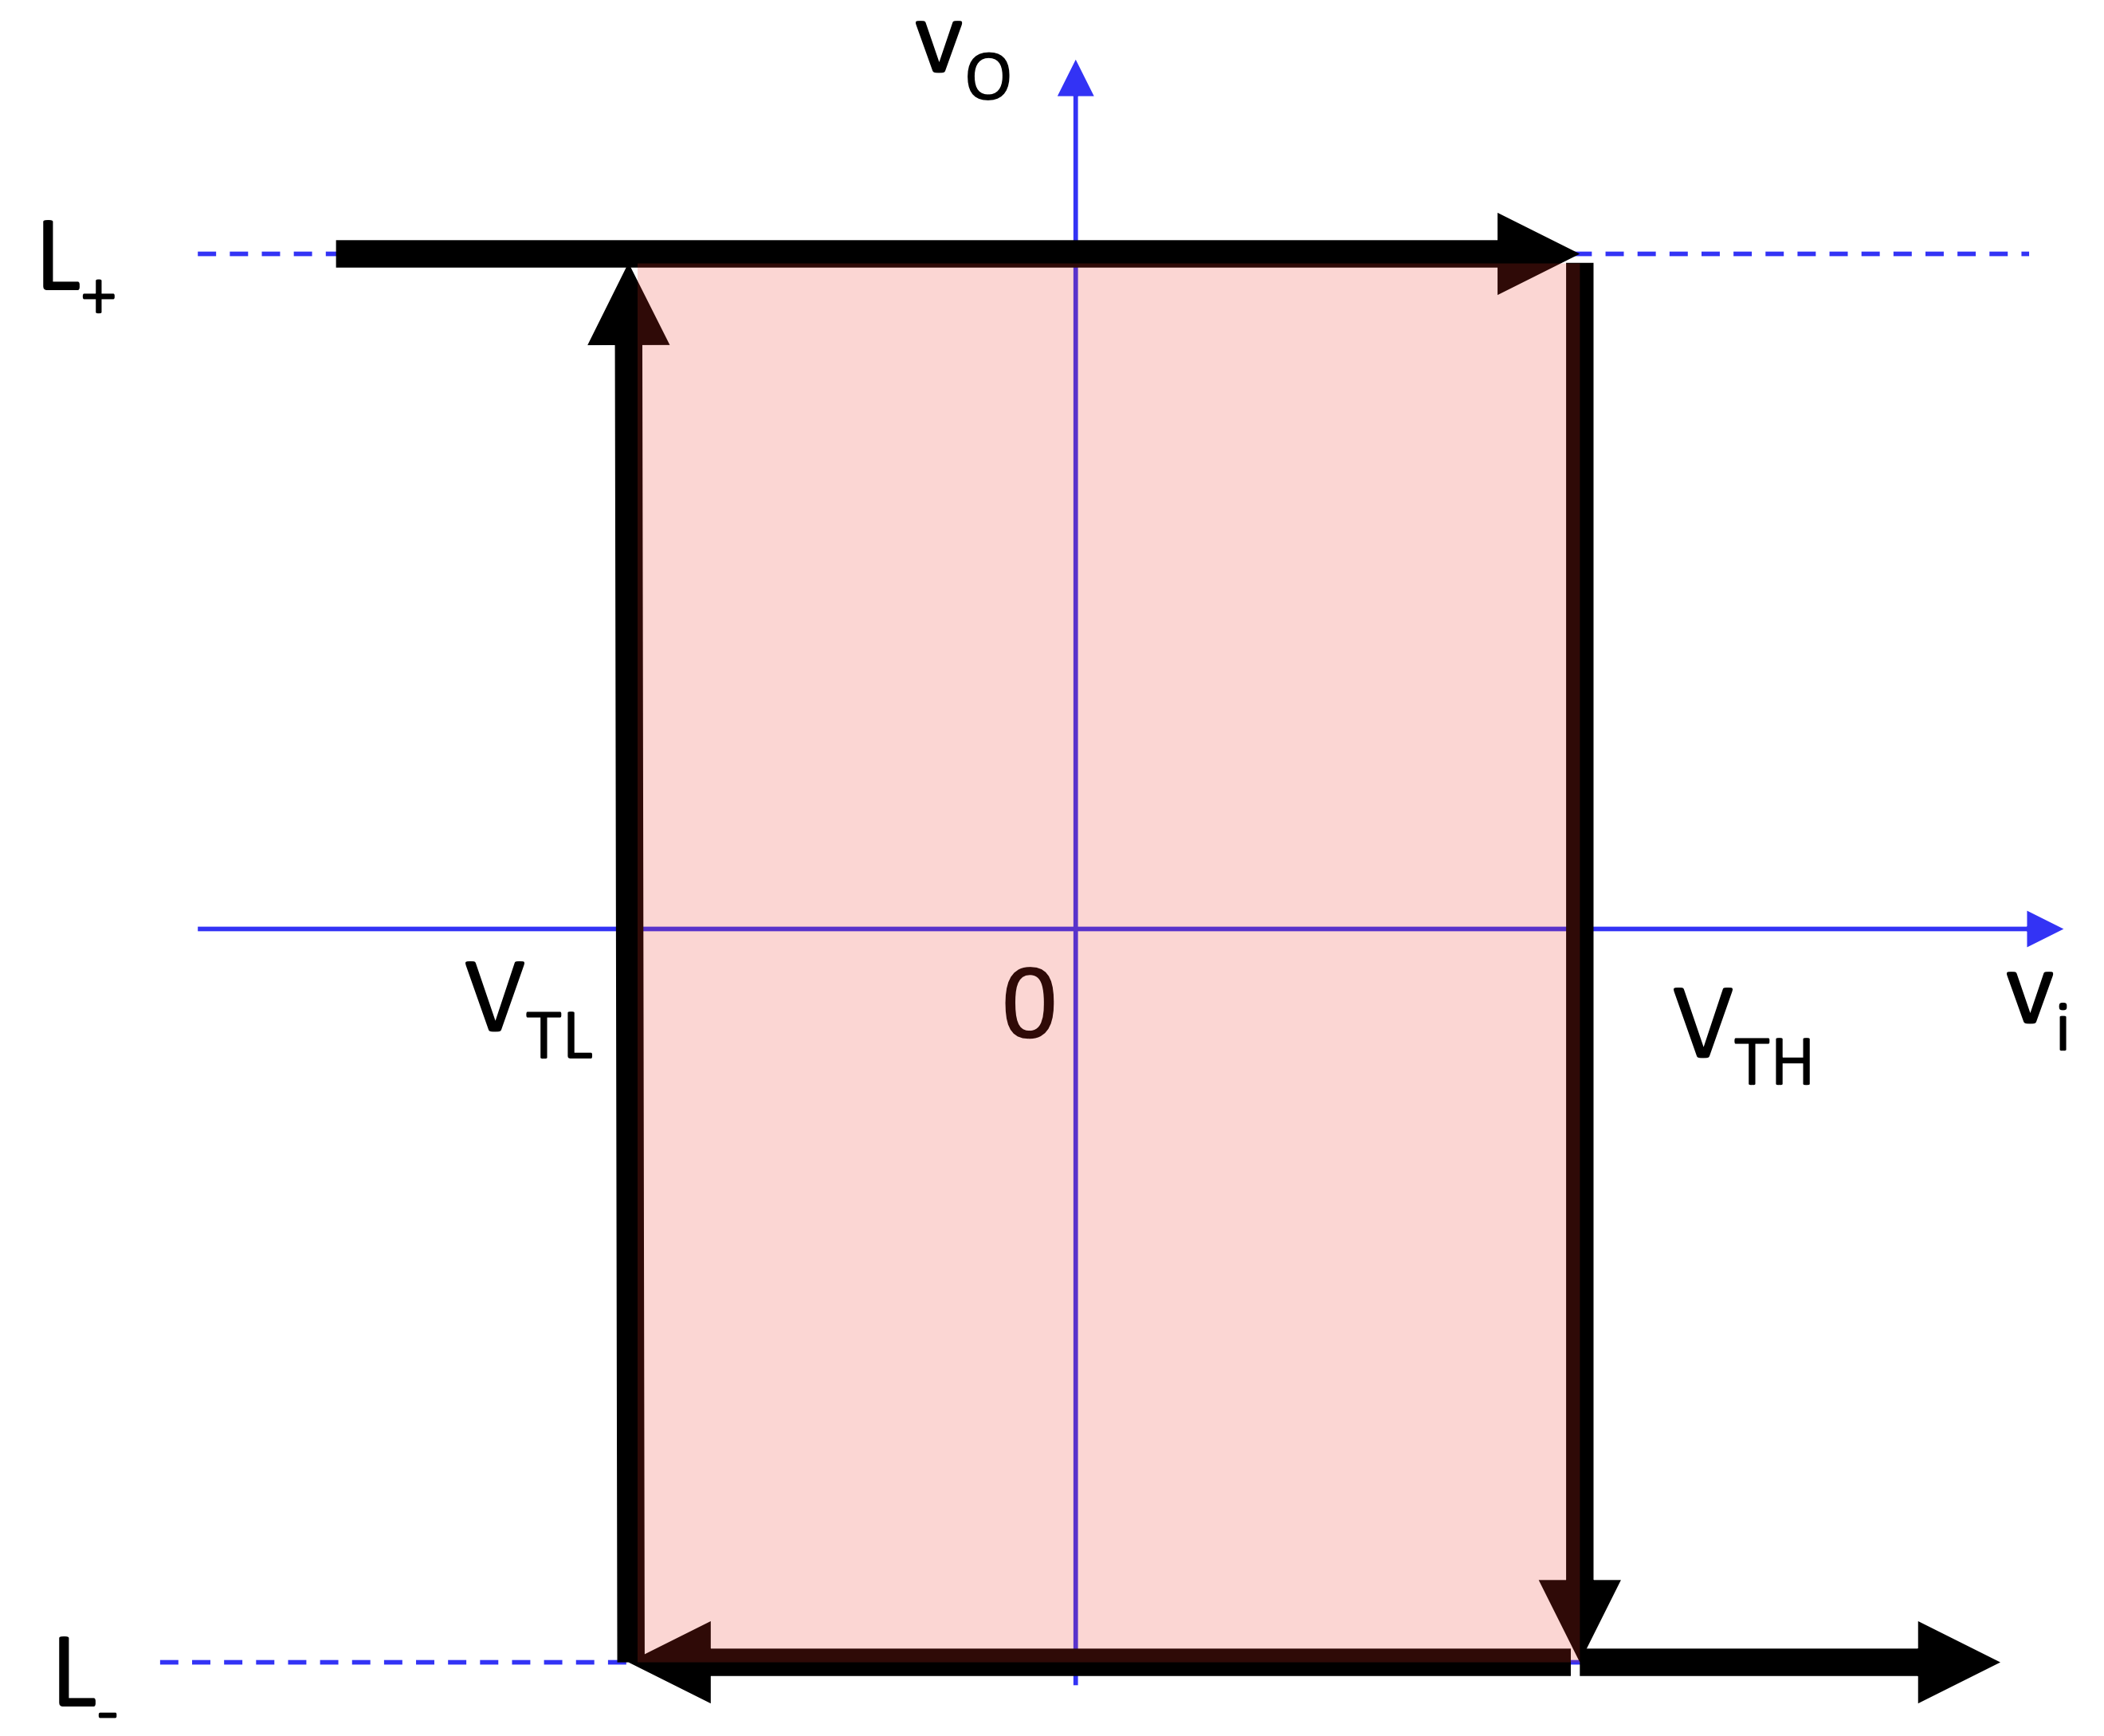
\includegraphics[width=0.7\textwidth]{immagini/inverting_bistable.png}
	\end{minipage}
\end{center}

\newpage

\subsubsection*{Non inverting bistable circuit}
A non inverting bistable circuit is a Schmitt trigger with a voltage generator (that acts as a trigger) connected at the end of
the voltage divider that feeds the non inverting input input of the op amp. It is called ``non inverting'' because the output
voltage is not inverted with respect to the input trigger voltage. 

The output voltage \(V_{out}\) will be at \(L_+\) and \(V_+ = L_+ \cdot R_1 / (R_1 + R_2) + V_{in} \cdot R_2 / (R_1 + R_2)\)
until the input trigger voltage \(V_{in}\) exceeds the negative threshold voltage \(V_{TL} = - L_+ \cdot R_1 / R_2\).
In this case the non-inverting input voltage \(V_+\) becomes negative, the output voltage \(V_{out}\) will switch to \(L_-\)
and \(V_+ = L_- \cdot R_1 / (R_1 + R_2) + V_{in} \cdot R_2 / (R_1 + R_2)\).

To switch back to \(L_+\), the input trigger voltage \(V_{in}\) must be bigger than the positive threshold voltage
\(V_{TH} = - L_- \cdot R_1 / R_2\). In this case the non inverting input voltage \(V_+\) become positive again to switch
the output back to \(L_+\).

\[V_{out} = L_+ \quad \Longleftrightarrow \quad V_+ = L_+ \cdot \frac{R_1}{R_1 + R_2} + V_{in} \cdot \frac{R_2}{R_1 + R_2} > 0 \quad \Longrightarrow \quad V_{in} > V_{TL} = -L_+ \cdot \frac{R_1}{R_2}\]
\[V_{out} = L_- \quad \Longleftrightarrow \quad V_+ = L_- \cdot \frac{R_1}{R_1 + R_2} + V_{in} \cdot \frac{R_2}{R_1 + R_2} < 0 \quad \Longrightarrow \quad V_{in} < V_{TH} = -L_- \cdot \frac{R_1}{R_2}\]

\begin{center}
	\begin{minipage}{0.45\textwidth}
		\centering \begin{circuitikz}[american, scale=0.8, transform shape]
			\draw (0,0) node[op amp, yscale=-1] (opamp) {};
			\node[ground] at (opamp.-) {}; 
			\node[left] at (opamp.+) {\(V_+\)};
			\draw (opamp.+) -- ++(0,1);
			\draw (opamp.out) to[short, -o] ++(0.5,0) node[right] {\(V_{out}\)};
			\draw (opamp.out) -- ++(0, 1.5)
			to[R, l=\(R_2\)] ++(-2.5, 0)
			to[R, l=\(R_1\)] ++(-2, 0) -- ++(-0.2,0)
			to[vsource, l_=\(V_{in}\)] ++(0, -1.5) ++(0, 0.3) node[ground] {};
		\end{circuitikz}
	\end{minipage}
	\begin{minipage}{0.45\textwidth}
		\centering 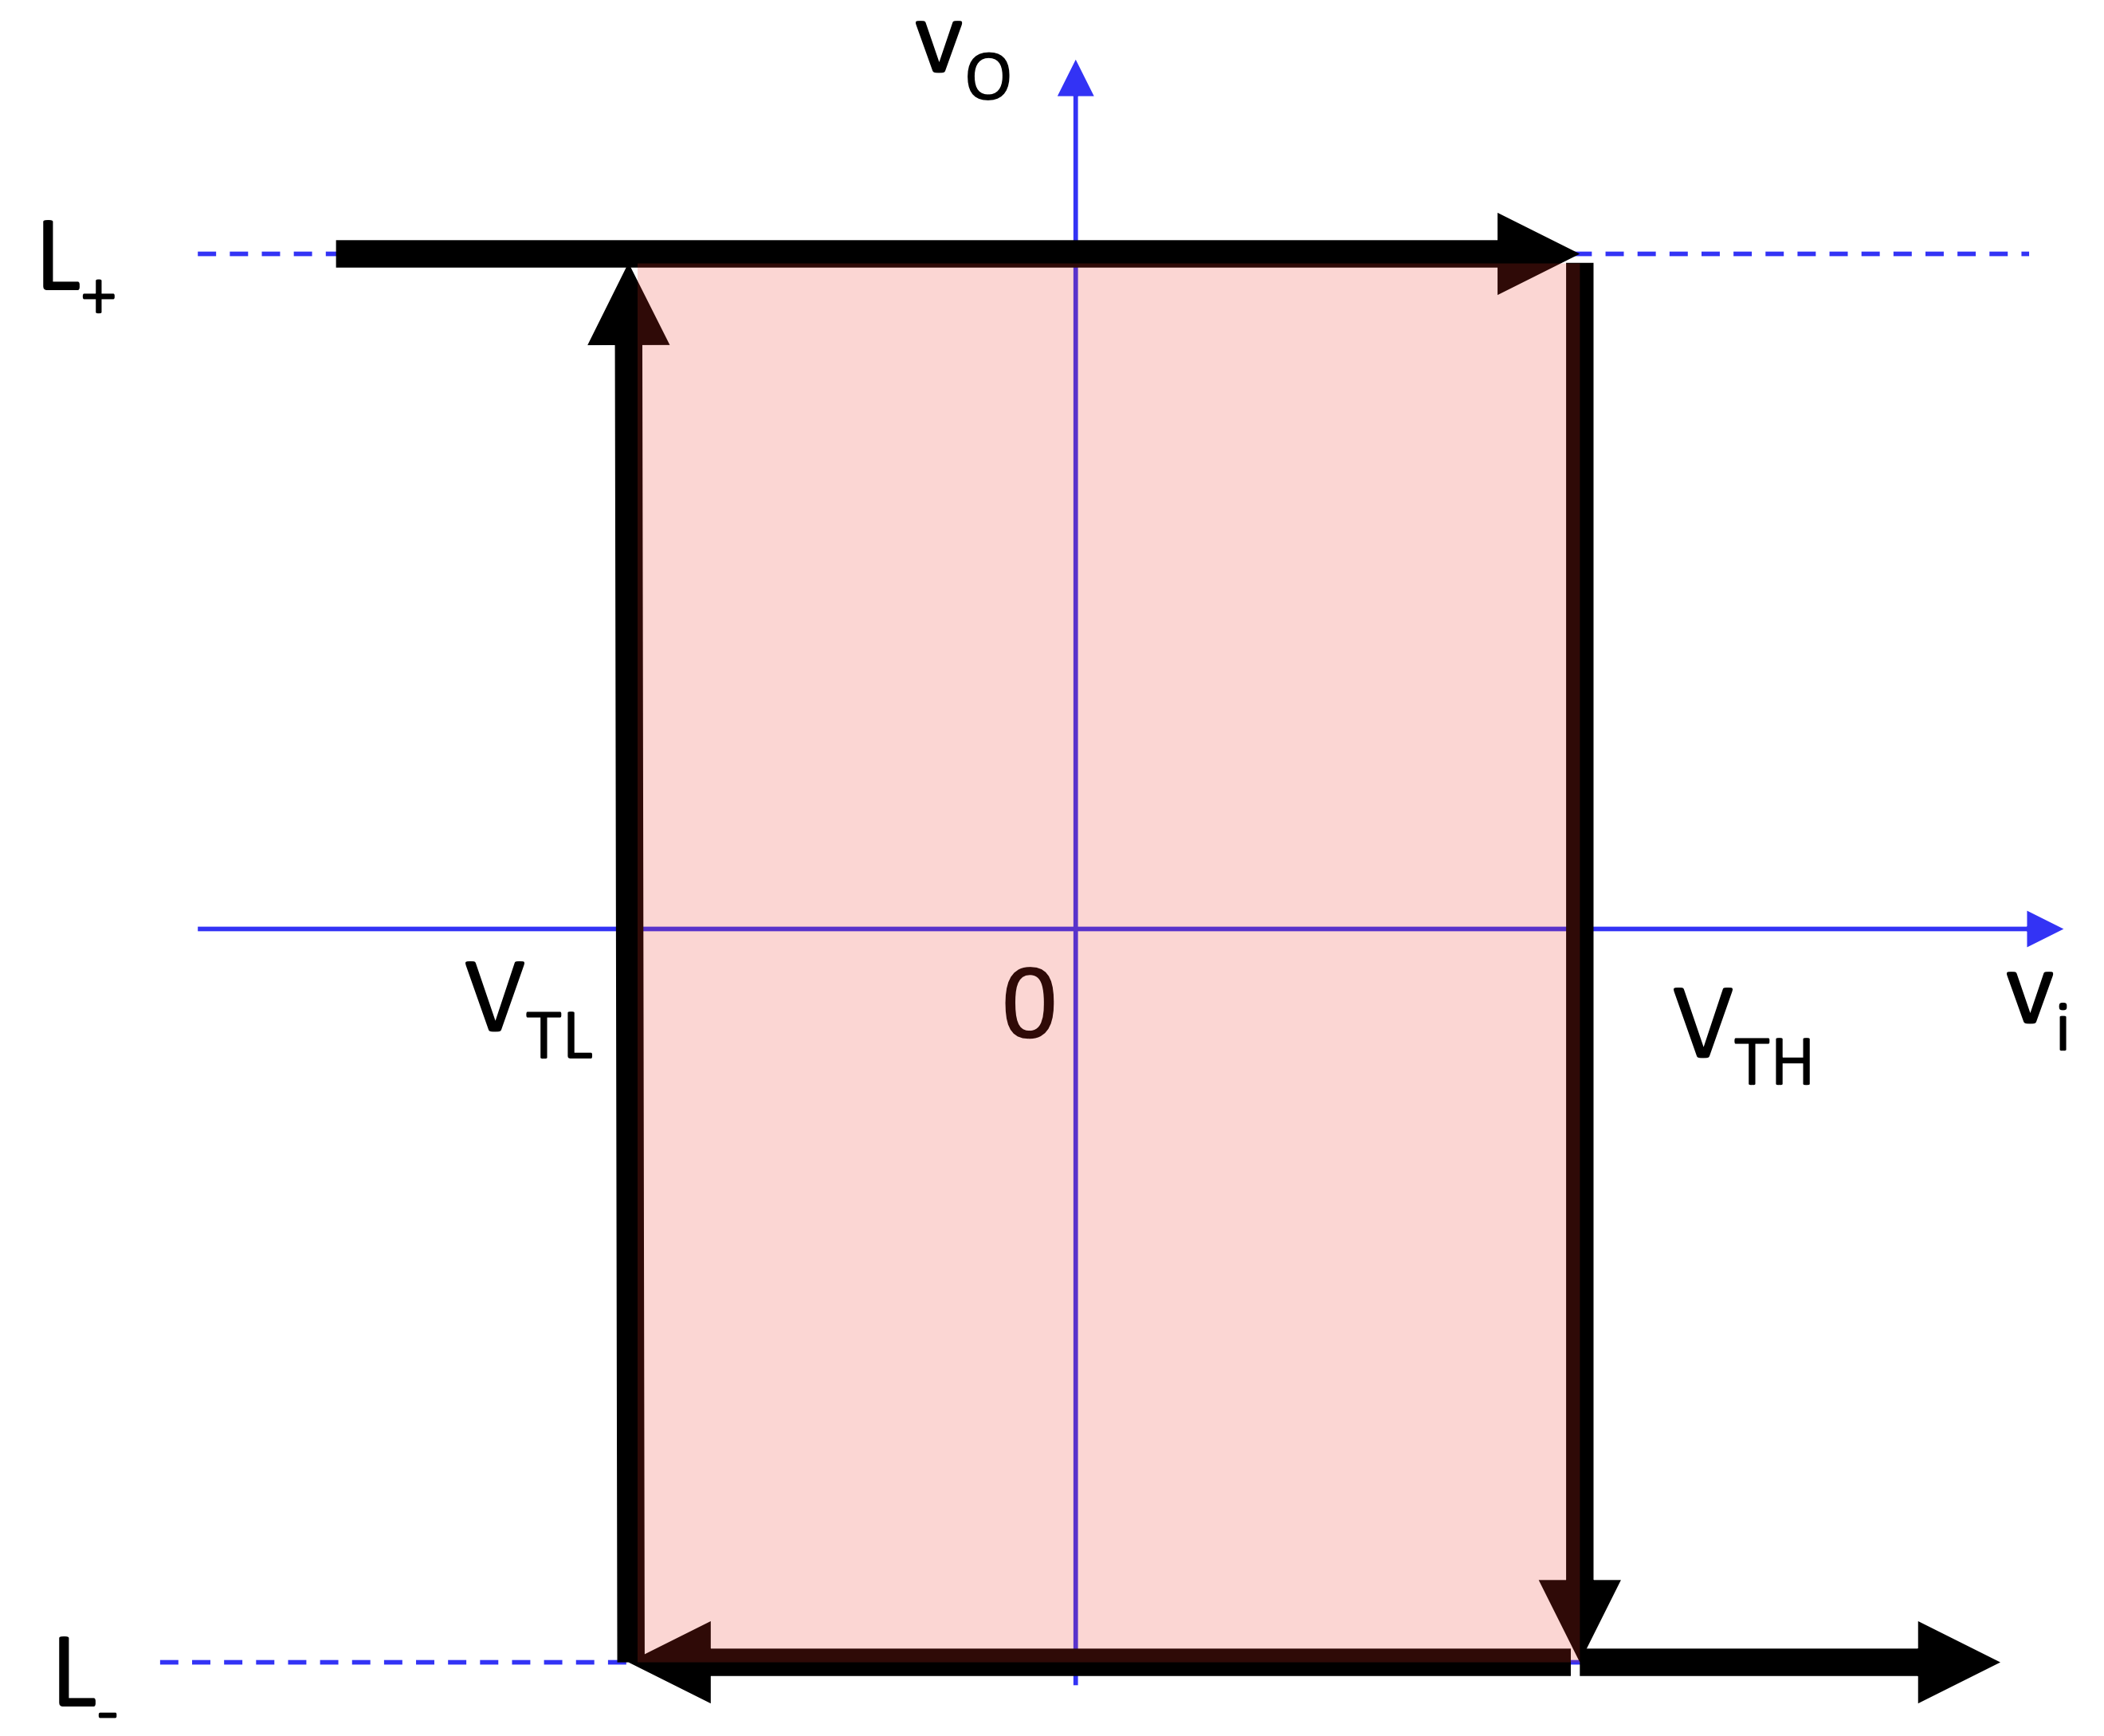
\includegraphics[width=0.7\textwidth]{immagini/inverting_bistable.png}
	\end{minipage}
\end{center}

\subsubsection*{Bistable circuit as a comparator}
The comparator is a circuit that compares two voltages and outputs a digital signal (high or low) depending on which voltage is
higher. Comparators can have hysteresis cycles (to mitigate the noise in input signal) and can be implemented with a bistable
circuit. They are usually used to:
\begin{itemize}
	\item detect signal levels with respect to a reference voltage
	\item convert an analog signal into a digital signal (analog to digital converter)
	\item implement a zero crossing detector (when the input signal crosses zero, the output changes state)
\end{itemize}

\newpage

\subsubsection*{Inverting bistable circuit with offset}
An inverting bistable circuit with offset is an inverting bistable circuit with threshold voltages that are shifted by a certain
defined offset voltage. This can be achieved by adding a second voltage generator to the non inverting input of the op amp and
a new resistor between the new voltage generator and the non inverting input.

The \(V_+\) non inverting input voltage is given by the superposition of new voltage generator and the op amp output voltage:
\[V_+ = V_R \cdot \frac{R_1 \parallel R_2}{R_1 \parallel R_2 + R_3} + V_{out} \cdot \frac{R_1 \parallel R_3}{R_1 \parallel R_3 + R_2}\]

Using the same reasoning as for the inverting bistable circuit, we can derive the new threshold voltages:
\begin{align*}
	V_{out} = L_+ \quad \Longleftrightarrow \quad &V_+ - V_{in} = V_R \cdot \frac{R_1 \parallel R_2}{R_1 \parallel R_2 + R_3} + L_+ \cdot \frac{R_1 \parallel R_3}{R_1 \parallel R_3 + R_2} - V_{in} > 0 \\
	\quad \Longrightarrow \quad &V_{in} < V_{TH} = V_R \cdot \frac{R_1 \parallel R_2}{R_1 \parallel R_2 + R_3} + L_+ \cdot \frac{R_1 \parallel R_3}{R_1 \parallel R_3 + R_2} \\
	V_{out} = L_- \quad \Longleftrightarrow \quad &V_+ - V_{in} = V_R \cdot \frac{R_1 \parallel R_2}{R_1 \parallel R_2 + R_3} + L_- \cdot \frac{R_1 \parallel R_3}{R_1 \parallel R_3 + R_2} - V_{in} < 0 \\
	\quad \Longrightarrow \quad &V_{in} > V_{TL} = V_R \cdot \frac{R_1 \parallel R_2}{R_1 \parallel R_2 + R_3} + L_- \cdot \frac{R_1 \parallel R_3}{R_1 \parallel R_3 + R_2}
\end{align*}

\begin{center}
	\begin{minipage}{0.45\textwidth}
		\centering \begin{circuitikz}[american, scale=0.8, transform shape]
			\draw (0,0) node[op amp, yscale=-1] (opamp) {};
			\node[left] at (opamp.+) {\(V_+\)};
			\draw (opamp.+) -- ++(0,1);
			\draw (opamp.out) to[short, -o] ++(0.5,0) node[right] {\(V_{out}\)};
			\draw (opamp.out) -- ++(0, 1.5)
			to[R, l=\(R_2\)] ++(-2.5, 0)
			to[short] node[pos=0.5] (r1top) {} ++(-1.5, 0)
			to[R, l=\(R_3\)] ++(-2, 0)
			to[vsource, l_=\(V_R\)] ++(0, -1.5) ++(0, 0.3) node[ground] {};
			\draw ($(r1top) + (0,0)$) to[R, l_=\(R_1\)] ++(0, -2)  node[ground] {};
			\draw (opamp.-) -- ++(-0.5, 0) to[vsource, l=\(V_{in}\)] ++(0, -1.5) ++(0, 0.3) node[ground] {};
		\end{circuitikz}
	\end{minipage}
	\begin{minipage}{0.45\textwidth}
		\centering 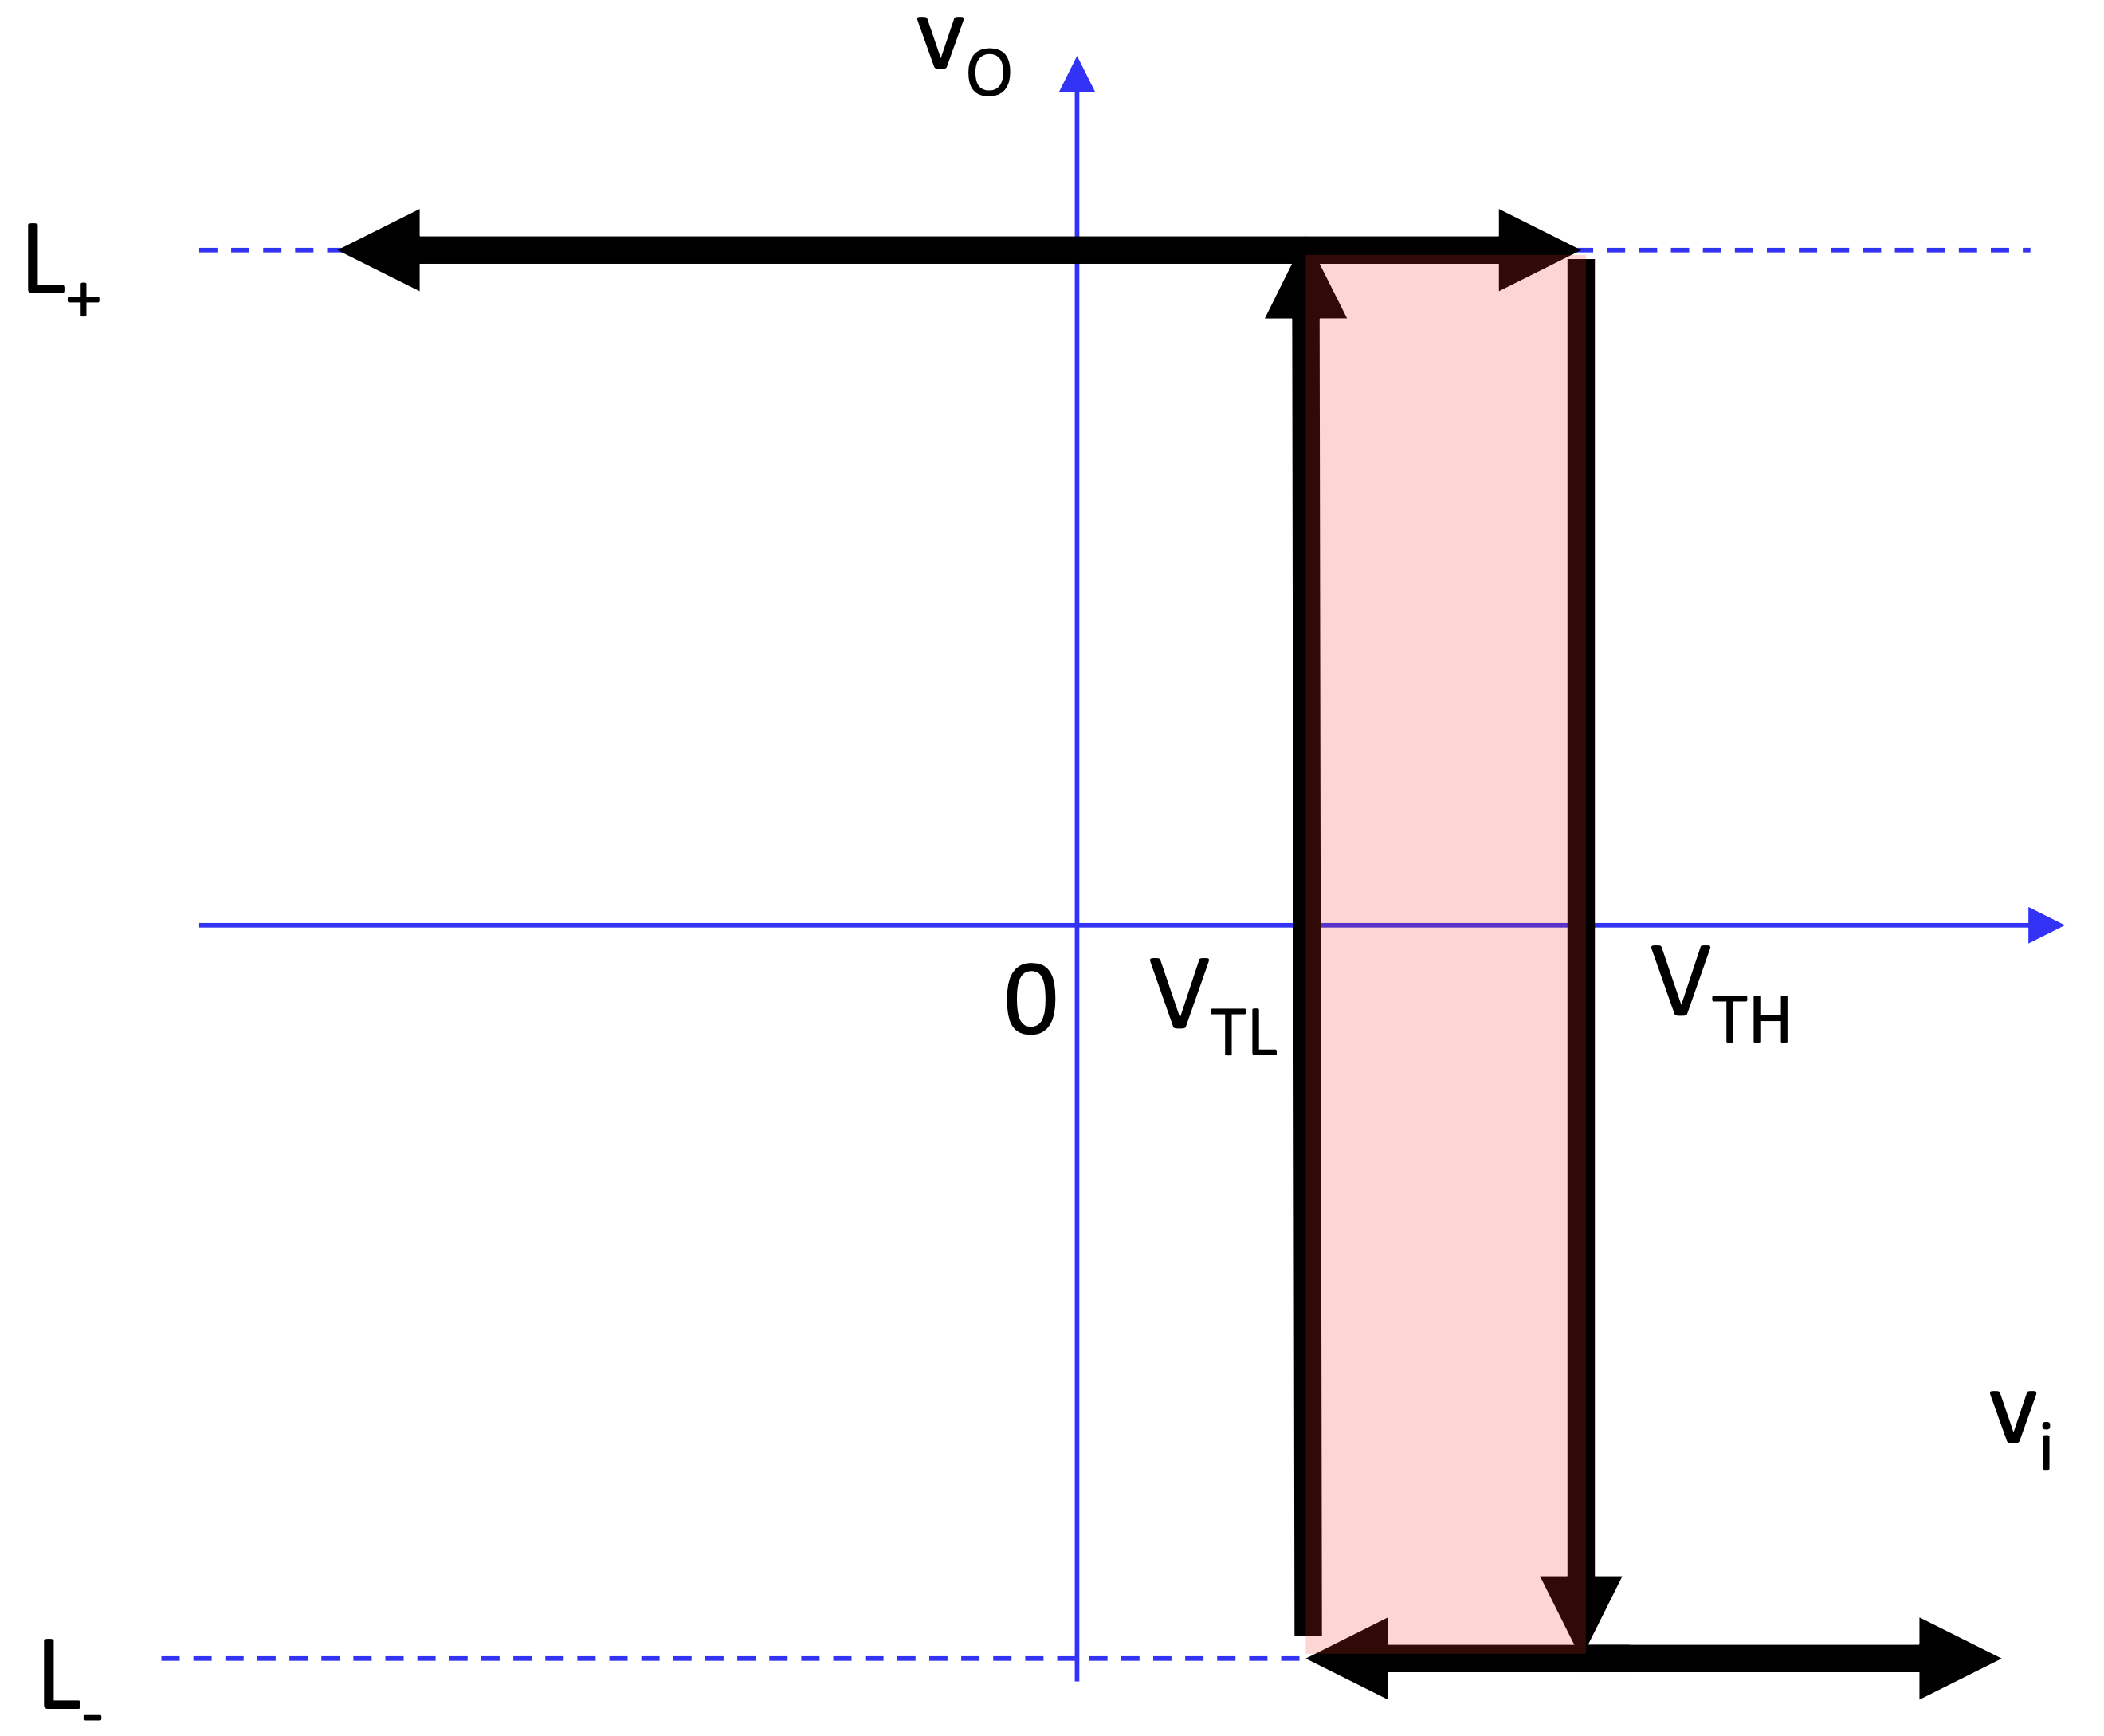
\includegraphics[width=0.7\textwidth]{immagini/inverting_bistable_offset.png}
	\end{minipage}
\end{center}

\subsubsection*{Fixed output voltage}
Saturation output voltages \(L_+\) and \(L_-\) of the op amp are not always defined and depend on the specific op amp used.
To fix the output voltage to a defined value, we can add two zener diodes face-to-face between output and ground. There is
also a resistor to bias the zener diodes and control the current through them.

Alternatively, we can use a 4-diode rectifier bridge to keep the zener diode in the correct orientation regardless of the
output voltage polarity.

\begin{center}
	\begin{minipage}{0.45\textwidth}
		\vspace{0.7cm}
		\centering \begin{circuitikz}[american, scale=0.8, transform shape]
			\ctikzset{diodes/scale=0.8}
			\draw (0,0) node[op amp, yscale=-1] (opamp) {};
			\node[ground] at (opamp.-) {}; 
			\node[left] at (opamp.+) {\(V_+\)};
			\draw (opamp.+) -- ++(0,1);
			\draw (opamp.out) to[R, l=\(R\)] ++(1.5,0) to[short, -o] ++(0.5,0) node[right] {\(V_{out}\)};
			\draw (opamp.out) ++(1.5,0) -- ++(0, 1.5) -- ++(-1.5,0)
			to[R, l=\(R_2\)] ++(-2.5, 0)
			to[R, l=\(R_1\)] ++(-2, 0) -- ++(-0.2,0)
			to[vsource, l_=\(V_{in}\)] ++(0, -1.5) ++(0, 0.3) node[ground] {};
			\draw (opamp.out) ++(1.5,0)
			to[zzDo] ++(0, -1.5) ++(0,-1.2)
			to[zzDo] ++(0, 1.5) ++(0,-1.1) node[ground] {};
		\end{circuitikz} \\[5pt]
		\footnotesize Bistable circuit with fixed output voltage using two zener diodes
	\end{minipage}
	\begin{minipage}{0.45\textwidth}
		\centering \begin{circuitikz}[american, scale=0.8, transform shape]
			\ctikzset{diodes/scale=0.8}
			\draw (0,0) node[op amp, yscale=-1] (opamp) {};
			\node[ground] at (opamp.-) {}; 
			\node[left] at (opamp.+) {\(V_+\)};
			\draw (opamp.+) -- ++(0,1);
			\draw (opamp.out) to[R, l=\(R\)] ++(1.5,0) to[short, -o] ++(0.5,0) node[right] {\(V_{out}\)};
			\draw (opamp.out) ++(1.5,0) -- ++(0, 1.5) -- ++(-1.5,0)
			to[R, l=\(R_2\)] ++(-2.5, 0)
			to[R, l=\(R_1\)] ++(-2, 0) -- ++(-0.2,0)
			to[vsource, l_=\(V_{in}\)] ++(0, -1.5) ++(0, 0.3) node[ground] {};
			\draw (opamp.out) ++(1.5,0) -- ++(0,-0.5) node (StartNode) {};

			\coordinate (DCplus)  at (StartNode);
			\coordinate (AC1)     at ([xshift=-1.4cm, yshift=-1.4cm]DCplus);
			\coordinate (DCminus) at ([xshift=1.4cm, yshift=-1.4cm]AC1);
			\coordinate (AC2)     at ([xshift=2.8cm, yshift=0cm]AC1);

			\draw (AC1) to[D] (DCplus); 
			\draw (AC1) to[D] (DCminus);
			\draw (DCminus) to[D] (AC2);
			\draw (DCplus) to[D] (AC2);
			\draw (AC1) to[zzDo] (AC2);
			\node[ground] at (DCminus) {};
		\end{circuitikz} \\[5pt]
		\footnotesize Bistable circuit with fixed output voltage using a diode bridge and a zener diode
	\end{minipage}
\end{center}

\newpage

\subsection{Triangular wave generator - Astable multivibrator}
\subsubsection*{Circuit}
Bistable circuits require an external trigger to switch between the two stable states. If we want to generate a periodic signal,
we can create a loop made of a bistable circuit and an integrator. The output of the bistable circuit is a square wave that feeds
the input of the integrator, which produces a triangular wave that feeds back the bistable circuit to switch its state. This
new auto-oscillating circuit is called astable multivibrator. It's important to use a non inverting bistable circuit with an
inverting integrator or vice versa to ensure oscillation.

\begin{center}
	\begin{minipage}{0.6\textwidth}
		\centering \begin{circuitikz}[american, scale=0.8, transform shape]
			\draw (0,0) node[op amp, yscale=-1] (opamp) {};
			\node[ground] at (opamp.-) {};
			\draw (opamp.out) to[short, -o] ++(0.5,0) node[right] {\(V_{out2}\)};
			\draw (opamp.out) node[circ] {} -- ++(0, 1.5)
				to[R, l=\(R_2\)] ++(-2.38, 0) -- (opamp.+);
			
			\draw (-5,0) node[op amp, yscale=-1] (opamp2) {};
			\draw (opamp2.+) -- ++(-0.5,0) node[ground] {};
			\draw (opamp2.out) to[short, -o] ++(0, 1) node[above] {\(V_{out1}\)};
			\draw (opamp2.out) -- ++(0, -1.5)
				to[C, name=c] ++(-2.38, 0);
			\draw (opamp.+) to[R, l=\(R_1\)] ++(-2, 0) to[short] (opamp2.out) node[circ] {};
			\draw (opamp2.-) -- ++(0, -2.5) to[R, name=r, i<=$I_R$] ++(2.38,0) -- ++(5,0) -- (opamp.out);

			\node at (c) [xshift=0.4cm, yshift=0.3cm, inner sep=1pt] {\(C\)};
			\node at (c) [xshift=0.7cm, yshift=-0.3cm, inner sep=1pt] (cminus) {\(-\)};
			\node at (c) [xshift=-0.7cm, yshift=-0.3cm, inner sep=1pt] (cplus) {\(+\)};
			\node at (r) [xshift=0.6cm, yshift=0.3cm, inner sep=1pt] {\(R\)};

			\draw[-{Latex}]
				($(cminus) + (-0.1, -0.2)$) to[out=-110, in=-70] 
				node[pos=0.5, fill=white, inner sep=1pt] {$V_C$} 
				($(cplus) + (0.1, -0.2)$);
		\end{circuitikz}
	\end{minipage}
	\begin{minipage}{0.35\textwidth}
		\centering 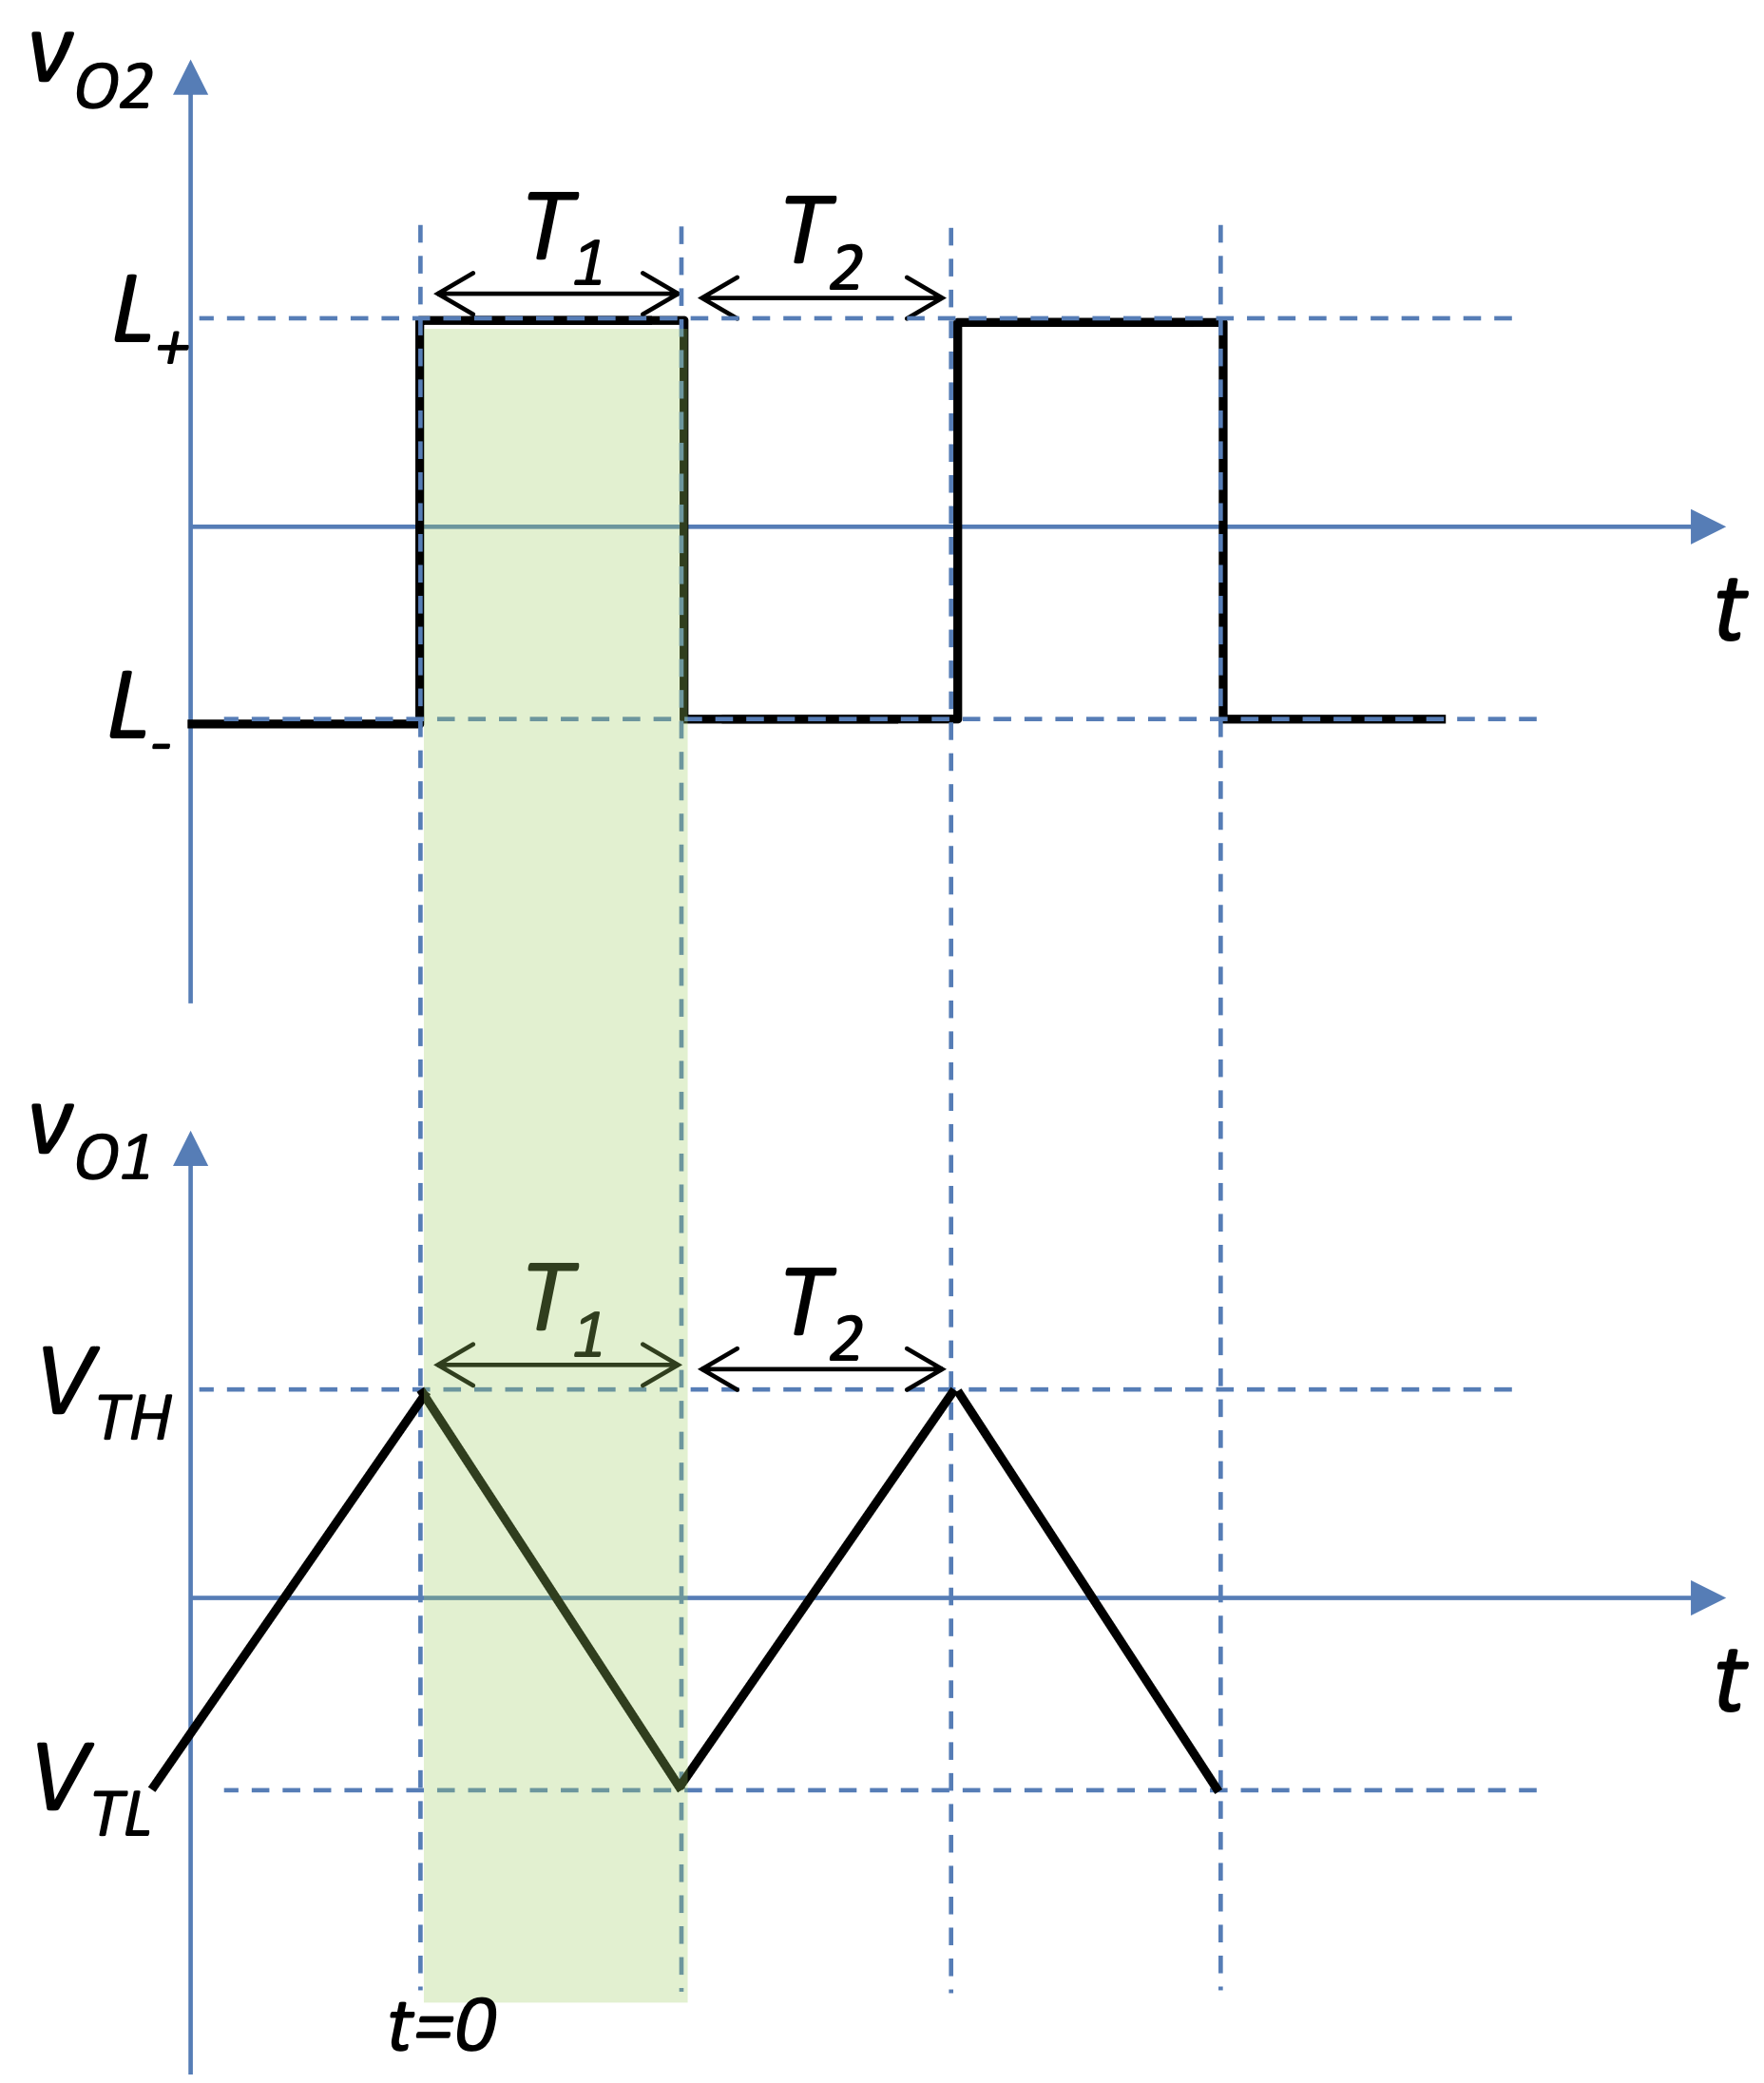
\includegraphics[width=0.8\textwidth]{immagini/astable_multivibrator.png}
	\end{minipage}
\end{center}

\subsubsection*{Circuit behaviour}
When \(V_{out2}\) is at \(L_+\), there is a constant current \(I_R = L_+ / R\) through the resistor \(R\) that discarge the
capacitor \(C\) at a constant rate of \(\frac{L_+}{RC}\). The output voltage \(V_{out1}\) decreases linearly with time, as
given by the following reasoning:
\[I_C = C \frac{dV_C}{dt} = - C \frac{dV_{out1}}{dt} = \frac{L_+}{R} \;\; \rightarrow \;\; V_{out1}(t) = V_{out1}(0) - \int \frac{L_+}{R} dt = V_{out1}(0) - \frac{L_+}{RC} t\]
When the output voltage \(V_{out1}\) reaches the negative threshold voltage \(V_{TL}\) of the bistable circuit, the output
voltage \(V_{out2}\) switches to \(L_-\) and the current through the resistor \(R\) becomes \(I_R = L_- / R\) (and changes sign).
The capacitor starts charging at a constant rate of \(\frac{L_-}{RC}\) and the output voltage \(V_{out1}\) increases linearly
until it reaches the positive threshold voltage \(V_{TH}\) of the bistable circuit that changes the output voltage \(V_{out2}\)
back to \(L_+\) and the cycle repeats indefinitely.

The period of the output signals is the time it takes for the output voltage \(V_{out1}\) to go from \(V_{TH}\) to \(V_{TL}\)
and back to \(V_{TH}\):
\begin{align*}
	\text{in } T_1, \; V_{out1} \text{ goes from } V_{TH} \text{ to } V_{TL}: \quad &\frac{V_{TH} - V_{TL}}{T_1} = \frac{L_+}{RC} \quad \rightarrow \quad T_1 = RC \frac{(V_{TH} - V_{TL})}{L_+} \\
	\text{in } T_2, \; V_{out1} \text{ goes from } V_{TL} \text{ to } V_{TH}: \quad &\frac{V_{TL} - V_{TH}}{T_2} = \frac{L_-}{RC} \quad \rightarrow \quad T_2 = RC \frac{(V_{TL} - V_{TH})}{L_-}
\end{align*}
If the bistable circuit is symmetric, with \(L_+ = L_-\), then the total period of the output signals is:
\[T = T_1 + T_2 = RC \frac{(V_{TH} - V_{TL})}{L_+} + RC \frac{(V_{TL} - V_{TH})}{L_-} = 2 RC \frac{(V_{TH} - V_{TL})}{L_+}\]

\newpage

\subsection{Sine wave generator}
By adding a bandpass filter to the triangular wave signal from the output of the astable multivibrator, it is possible to
attenuate the harmonics of the signal and keep the fundamental sine wave. The bandpass filter can be a first-order low-pass
filter implemented with an op amp. A first order low-pass filter may not be enough to obtain a good sine wave, because the third harmonic is
attenuated to 30\%, maybe a second order low-pass filter is needed.

\begin{center}
	\begin{minipage}{0.8\textwidth}
		\centering \begin{circuitikz}[american, scale=0.8, transform shape]
			\draw (0,0) node[op amp, yscale=-1] (opamp) {};
			\node[ground] at (opamp.-) {};
			\draw (opamp.out) to[short, -o] ++(0.5,0) node[right] {\(V_{out2}\)};
			\draw (opamp.out) node[circ] {} -- ++(0, 1.5)
				to[R, l=\(R_2\)] ++(-2.38, 0) -- (opamp.+);
			
			\draw (-5,0) node[op amp, yscale=-1] (opamp2) {};
			\draw (opamp2.+) -- ++(-0.5,0) node[ground] {};
			\draw (opamp2.out) to[short, -o] ++(0, 1) node[above] {\(V_{out1}\)};
			\draw (opamp2.out) -- ++(0, -1.5)
				to[C, name=c] ++(-2.38, 0);
			\draw (opamp.+) to[R, l=\(R_1\)] ++(-2, 0) to[short] (opamp2.out) node[circ] {};
			\draw (opamp2.-) -- ++(0, -2) to[R, name=r] ++(2.38,0) -- ++(5,0) -- (opamp.out);

			\node at (c) [xshift=0.4cm, yshift=0.3cm, inner sep=1pt] {\(C\)};
			\node at (r) [xshift=0.6cm, yshift=0.3cm, inner sep=1pt] {\(R\)};

			\draw (6,0) node [op amp] (opamp3) {};
			\draw (opamp3.+) node[ground] {};
			\draw (opamp3.out) to[short, -o] ++(0.5,0) node[right] {\(V_{out3}\)};
			\draw (opamp3.out) -- ++(0, 1.5)
				to[C, name=c4] ++(-2.38, 0) -- (opamp3.-);
			\draw (opamp3.out) -- ++(0, 2.5)
				to[R, name=r4] ++(-2.38, 0) -- (opamp3.-);
			\draw (opamp3.-) to[R, l=\(R_3\)] ++(-2, 0) -- ++(-1,2) to[short] ++(-4.4,0) to[short] (opamp2.out);
			
			\node at (c4) [xshift=0.4cm, yshift=0.3cm, inner sep=1pt] {\(C_4\)};
			\node at (r4) [xshift=0.6cm, yshift=0.3cm, inner sep=1pt] {\(R_4\)};
		\end{circuitikz}
	\end{minipage}
\end{center}

The trasnfer characteristic of the low-pass filter is given by:
\[H(j\omega) = \frac{V_{out3}}{V_{in3}} = -\frac{Z_f}{Z_{in}} = - \frac{R_4 \cdot Z_{C4}}{R_4 + Z_{C4}} \cdot \frac{1}{R_3} = - \frac{R_4 / j\omega C_4}{R_4 + 1 / j\omega C_4} \cdot \frac{1}{R_3} = \underbrace{- \frac{R_4}{R_3}}_{\text{\footnotesize gain}} \cdot \underbrace{\frac{1}{1 + j\omega R_4 C_4}}_{\text{\footnotesize low-pass filter}}\]
\[\left|H(j\omega)\right| = \left|\cdot \frac{1}{\sqrt{1 + (\omega R_4 C_4)^2}}\right| = \frac{1}{\sqrt{2}} \quad \rightarrow \quad \omega = \frac{1}{R_4 C_4} \quad \rightarrow \quad f_c = \frac{1}{2\pi R_4 C_4}\]

\section{Output stages}
\subsection{Introduction}
\subsubsection*{Goal}
Due to the maximum current limits of the op amps, they cannot be used to drive loads (speakers) directly. A power amplifier is
needed to preserve the same signal waveform, but with higher current and power. A good power amplifier should have:
\begin{itemize}
	\item support for large signal operation (10-20 V)
	\item low output impedance (to drive low impedance loads with high efficiency)
	\item low harmonic distortion (to preserve the signal waveform)
\end{itemize}

\subsubsection*{Power amplifiers classes}
\begin{itemize}
	\item class A: the output stage is always on, even without input signal
	\item class B: the output stage is on only for half of the input signal period
	\item class AB: the output stage is on for more than half of the input signal period
	\item class C: the output stage is on for less than half of the input signal period
\end{itemize}

\subsubsection*{THD - Total Harmonic Distortion}
The total harmonic distortion (THD) is a measure of the quality of the output signal. It is defined as the ratio of the RMS power
of the entire harmonic content (excluding the fundamental frequency) of the output signal to the RMS power of the fundamental
frequency.
\[THD = \frac{\sqrt{{V_2}^2 + {V_3}^2 + {V_4}^2 + \cdots}}{V_1} = \frac{\sqrt{\sum_{i \geq 2} {V_i}^2}}{V_1}\]

\subsection{Class A - Emitter follower}
\subsubsection*{Circuit description}
The simplest class A output stage is the emitter follower, which is a BJT transistor in which the input signal is applied to
the base and the output is taken from the emitter. The collector is connected to the supply voltage. This configuration is
called ``emitter follower'' because the output voltage in the emitter follows the input voltage at the base, with a fixed
voltage drop \(V_{BE}\). The transistor acts also as a current amplifier to drive the load with appropriate power.
\[V_{out} = V_{in} - V_{BE} \qquad\qquad I_E = \beta I_B\]

To ensure that the transistor is always on, there must be a bias current flowing from the emitter, even without input signal.
This can be achieved by using a current generator connected between the emitter and ground. The generator current \(I_{gen}\)
must be higher than the maximum current \(I_{L,max}\) that can be delivered to the load, to ensure that \(I_E\) current is
always positive.
\[I_{E} = I_{gen} + I_L > 0 \quad \rightarrow \quad I_{gen} > \left|I_L\right|\]

\begin{center}
	\begin{minipage}{0.5\textwidth}
		\centering\begin{circuitikz}[american, scale=0.8, transform shape]
			\node[npn] (Q1) at (0,0) {};
			\node[right] at (Q1) {$Q_1$};
			\draw (Q1.B) to[short, -o] ++(-0.5,0) node[left] {$V_{in}$};
			\draw (Q1.C) to[short, -o] ++(0,0) node[above] {$+V_{CC}$};
			\draw (Q1.E) to[short, i=\(I_{E}\)] ++(0,-0.5) coordinate (outSplit);
			\draw (outSplit) -- ++(0.5,0) to[short, -o, i_=\(I_L\)] ++(1,0) node[right] {$V_{out}$}
				to[R, l=\(R_L\)] ++(0, -2) ++(0,0.4)node[ground] {};
			\draw (outSplit) to[isource, l_=$I_{gen}$, -o] ++(0,-1.5) node[below] {$-V_{CC}$};
	
			\node [xshift=-0.1cm, yshift=-0.2cm] at (Q1.B) (vplus) {$+$};
			\node [xshift=-0.3cm, yshift=-0.3cm] at (Q1.E) (vminus) {$-$};
			\draw (vminus) to node[midway, fill=white, inner sep=3pt] {$V_{BE}$} (vplus);
		\end{circuitikz}
	\end{minipage}
\end{center}

\subsubsection*{With diode to bias transistor}
It is possible implement the ideal current generator by using a diode with a fixed voltage drop \(V_D\) to impose a fixed voltage
drop \(V_{BE2} = V_D\) across the transistor \(Q_2\) that generates the constant current \(I_{gen}\).

The problem is that small variations on the voltage \(V_D\) (due to component heating) are exponentially amplified in current
variations \(I_{gen}\) by the transistor \(Q_2\) and the output stage becomes unstable.

\begin{center}
	\begin{minipage}{0.4\textwidth}
		\centering \begin{circuitikz}[american, scale=0.8, transform shape]
			\ctikzset{diodes/scale=0.8}
			\node[npn] (Q1) at (0,0) {\(Q_1\)};
			\draw (Q1.B) to[short, -o] ++(-0.5,0) node[left] {$V_{in}$};
			\draw (Q1.C) to[short, -o] ++(0,0) node[above] {$+V_{CC}$};
			\draw (Q1.E) to[short, i=\(I_{E}\)] ++(0,-0.5) coordinate (outSplit);
			\draw (outSplit) -- ++(0.5,0) to[short, -o, i_=\(I_L\)] ++(1,0) node[right] {$V_{out}$}
				to[R, l=\(R_L\)] ++(0, -2) ++(0,0.4)node[ground] {};
			
			\node[npn, anchor=collector] at (outSplit) (Q2) {\(Q_2\)};
			\draw (Q2.E) to[short, -o, i=\(I_{gen}\)] ++(0,-0.7) node[below] {$-V_{CC}$};

			\draw (Q2.B) -- ++(-2,0) to[D, l=\(D\)] ++(0,-1.5) to[short, -o] ++(0,0) node[below] {$-V_{CC}$};
			\draw (Q2.B) -- ++(-2,0) to[R, l_=\(R\)] ++(0,1.5) to[short] ++(0,0) node[ground, yscale=-1] {};
	
			\node [xshift=-0.1cm, yshift=-0.2cm] at (Q1.B) (vplus) {$+$};
			\node [xshift=-0.3cm, yshift=-0.3cm] at (Q1.E) (vminus) {$-$};
			\draw (vminus) to node[midway, fill=white, inner sep=3pt] {$V_{BE1}$} (vplus);

			\node [xshift=-0.1cm, yshift=-0.2cm] at (Q2.B) (vplus) {$+$};
			\node [xshift=-0.3cm, yshift=-0.3cm] at (Q2.E) (vminus) {$-$};
			\draw (vminus) to node[midway, fill=white, inner sep=3pt] {$V_{BE2}$} (vplus);
		\end{circuitikz}
	\end{minipage}
	\begin{minipage}{0.45\textwidth}
		\[I_{gen} = I_{C2} = I_S \left( e^{V_{BE2} / V_T} - 1 \right)\]
	\end{minipage}
\end{center}

\subsubsection*{With current mirror transistors}
The idea is to use a current mirror to generate the bias current \(I_{gen}\) for the output stage. The current mirror is made
of two matched transistors \(Q_2\) and \(Q_3\) that share the same base voltage \(V_{BE2} = V_{BE3}\) and therefore the same
working point. The current \(I_{gen}\) is set by the resistor \(R\) and the voltage drop \(V_{BE3}\) across the transistor \(Q_3\).

The problem of this configuration is that the current mirror transistor should be matched (should come from the same silicon wafer)
and sometimes this requirement is impossible to achieve.

\begin{center}
	\begin{minipage}{0.4\textwidth}
		\centering\begin{circuitikz}[american, scale=0.8, transform shape]
			\node[npn] (Q1) at (0,0) {\(Q_1\)};
			\draw (Q1.B) to[short, -o] ++(-0.5,0) node[left] {$V_{in}$};
			\draw (Q1.C) to[short, -o] ++(0,0) node[above] {$+V_{CC}$};
			\draw (Q1.E) to[short, i=\(I_{E}\)] ++(0,-0.5) coordinate (outSplit);
			\draw (outSplit) -- ++(0.5,0) to[short, -o, i_=\(I_L\)] ++(1,0) node[right] {$V_{out}$}
				to[R, l=\(R_L\)] ++(0, -2) ++(0,0.4)node[ground] {};
			
			\node[npn, anchor=collector] at (outSplit) (Q2) {\(Q_2\)};
			\node[npn, anchor=base, xshift=-0.5cm, xscale=-1] at (Q2.B) (Q3) {};
			\node[left] at (Q3) {\(Q_3\)};
			\draw (Q3.B) -- (Q2.B);
			\draw (Q2.E) to[short, -o, i=\(I_{gen}\)] ++(0,-0.7) node[below] {$-V_{CC}$};
			\draw (Q3.E) to[short, -o, i_=\(I_{gen}\)] ++(0,-0.7) node[below] {$-V_{CC}$};

			\draw (Q3.C) -- ++(0.6,0) -- (Q3.B);
			\draw (Q3.C) to[R, l_=\(R\)] ++(-2,0) node[ground] {};
	
			\node [xshift=-0.1cm, yshift=-0.2cm] at (Q1.B) (vplus) {$+$};
			\node [xshift=-0.3cm, yshift=-0.3cm] at (Q1.E) (vminus) {$-$};
			\draw (vminus) to node[midway, fill=white, inner sep=3pt] {$V_{BE1}$} (vplus);

			\node [xshift=-0cm, yshift=-0.2cm] at (Q2.B) (vplus) {$+$};
			\node [xshift=-0.3cm, yshift=-0.3cm] at (Q2.E) (vminus) {$-$};
			\draw (vminus) to node[midway, fill=white, inner sep=3pt] {$V_{BE2}$} (vplus);

			\node [xshift=0cm, yshift=-0.2cm] at (Q3.B) (vplus) {$+$};
			\node [xshift=0.3cm, yshift=-0.3cm] at (Q3.E) (vminus) {$-$};
			\draw (vminus) to node[midway, fill=white, inner sep=3pt] {$V_{BE3}$} (vplus);
		\end{circuitikz}
	\end{minipage}
	\begin{minipage}{0.45\textwidth}
		\[I_{gen} = I_R = \frac{V_R}{R} = \frac{\left|-V_{CC}\right| - V_{BE3}}{R}\]
	\end{minipage}
\end{center}

\subsubsection*{Transfer characteristic}
The transfer characteristic of the emitter follower is a straight line with a slope of 1 and a vertical offset of \(-V_{BE1}\).
The upper limit of the output voltage is \(V_{CC} - V_{CE1sat}\) that occurs when the transistor \(Q_1\) is in saturation. The
lower limit of the output voltage is the minimum (in absolute value) between \(-V_{CC}+V_{CE2sat}\) (saturation of \(Q_2\)) and
\(-I_{gen} \cdot R_L\) (maximum load current before \(Q_1\) enters cutoff).

\begin{center}
	\begin{minipage}{0.45\textwidth}
		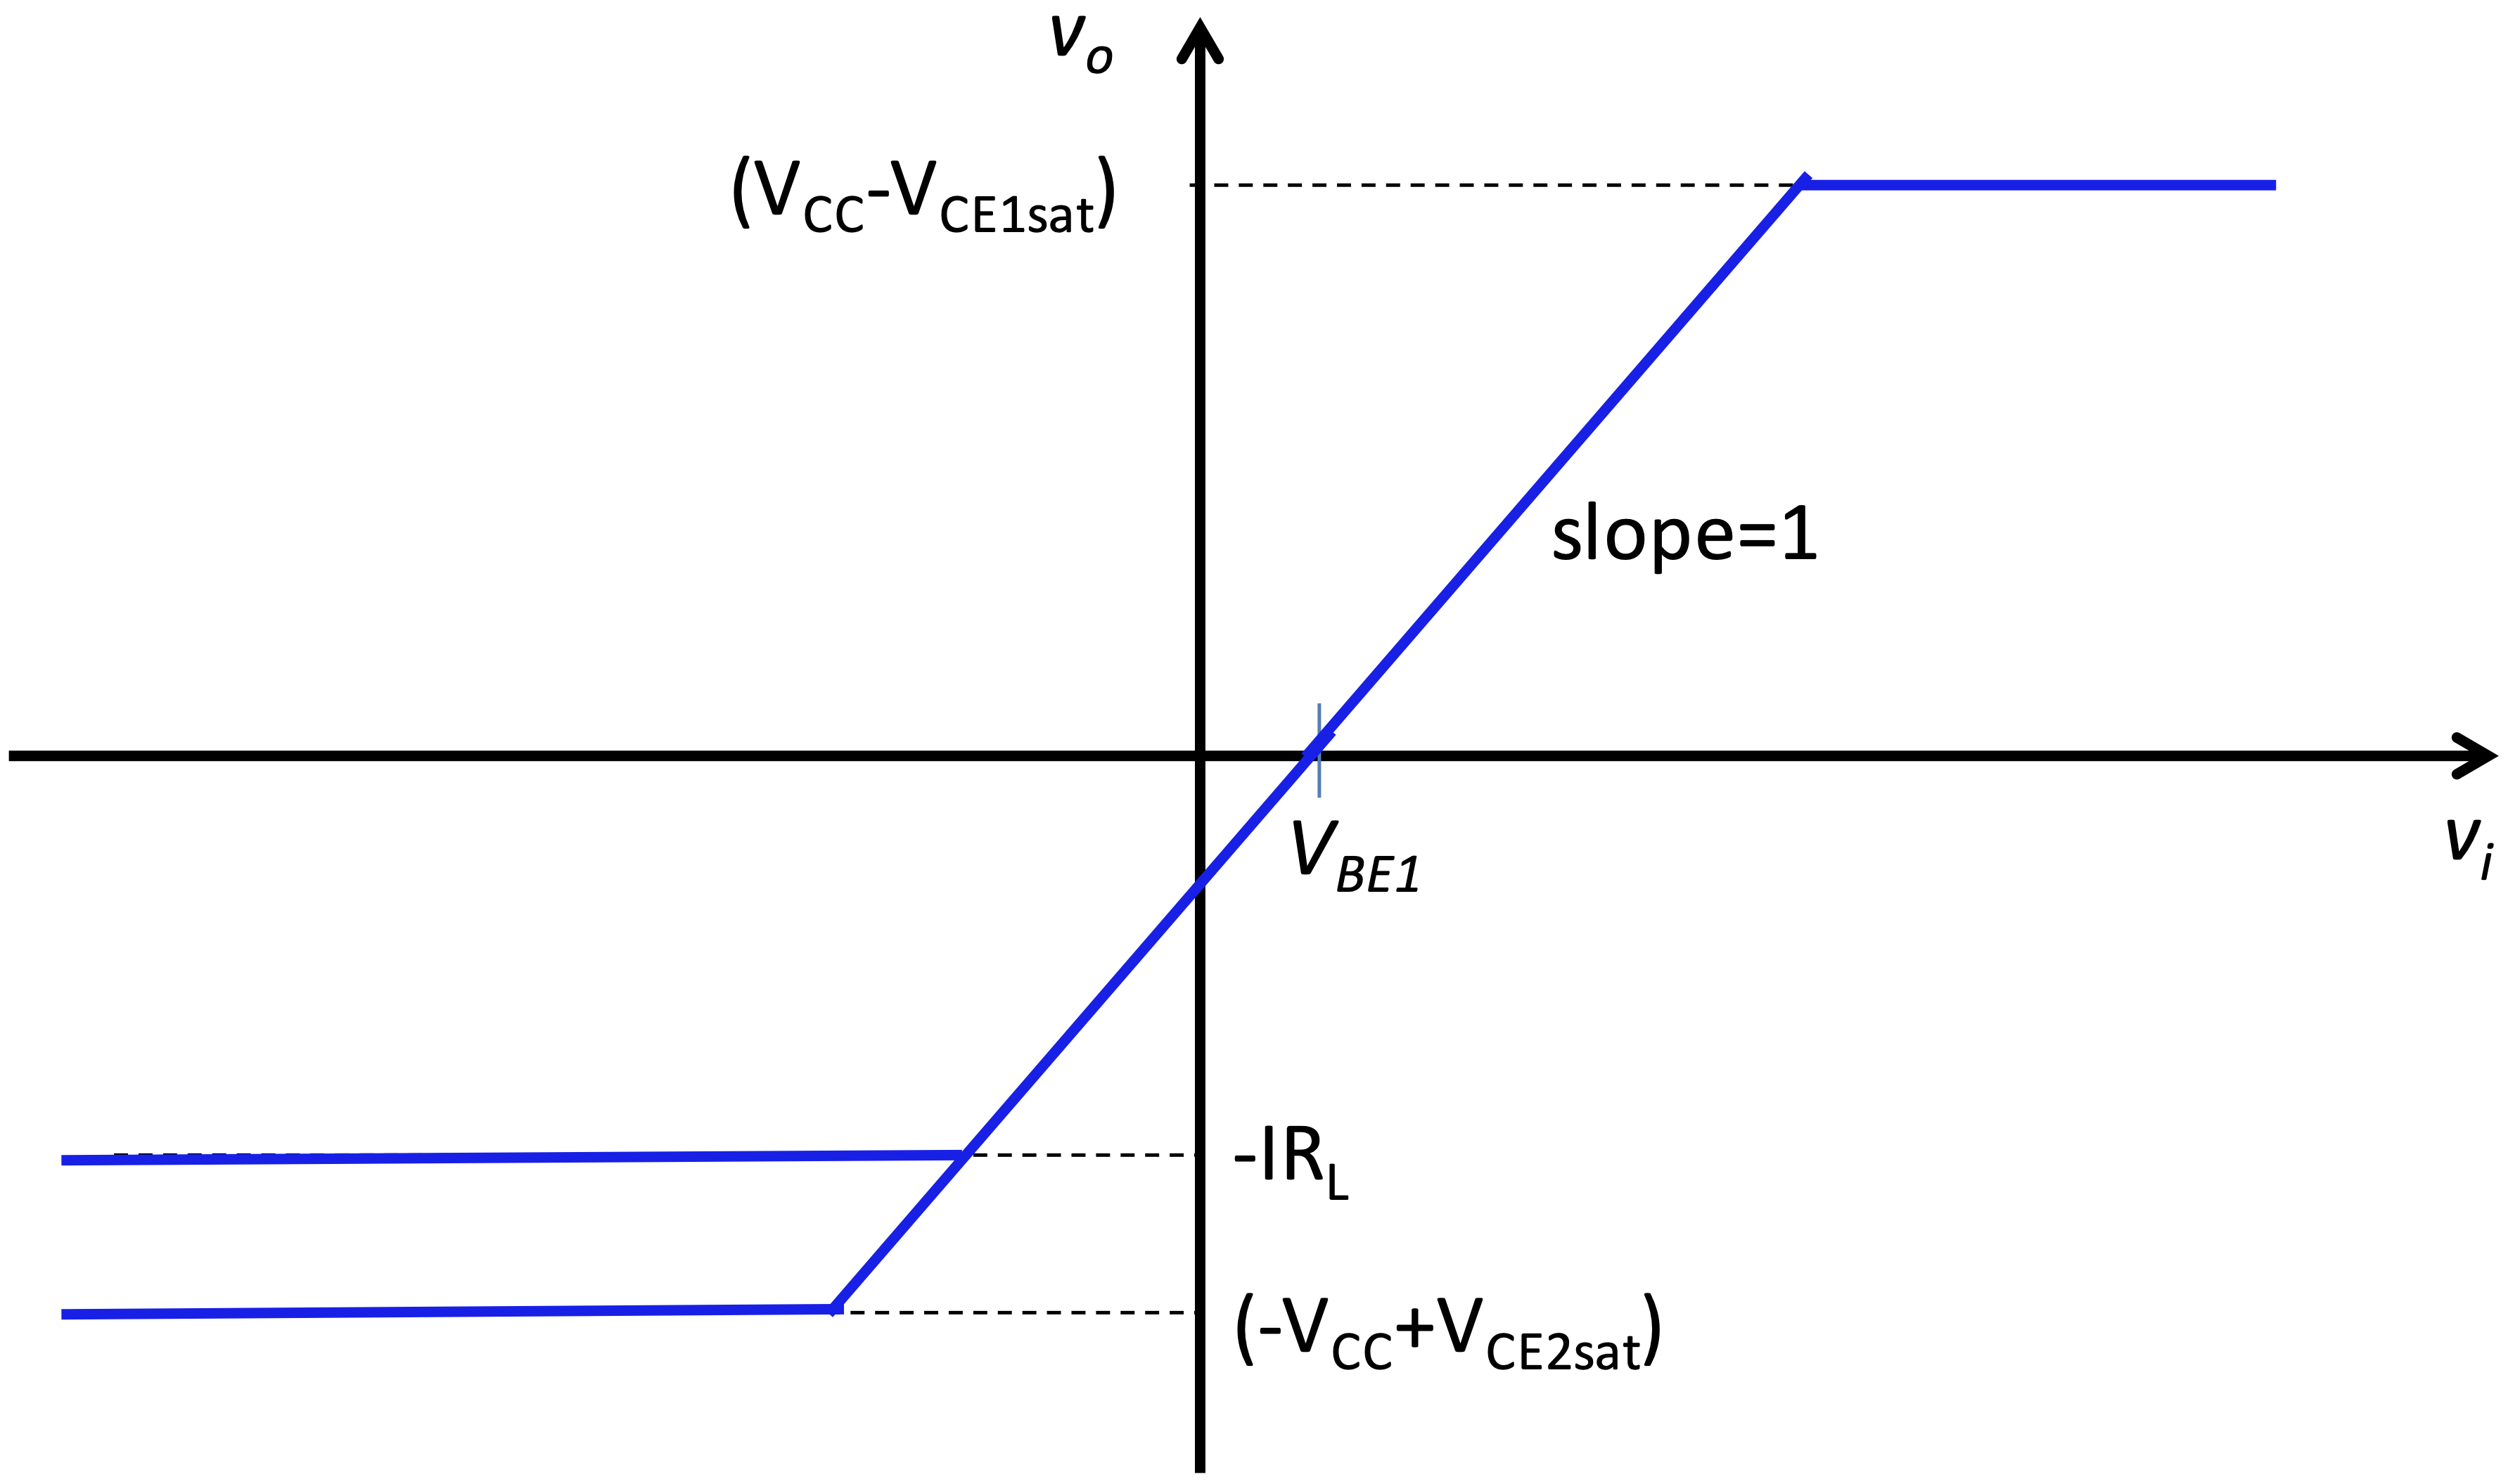
\includegraphics[width=\textwidth]{immagini/class_a_characteristic.png}
	\end{minipage}
	\begin{minipage}{0.5\textwidth}
		\begin{align*}
			V_{out} &= V_{in} - V_{BE1} \\
			& \\
			V_{out,max} &= V_{CC} - V_{CE1sat} \\
			V_{out,min} &= \max \left\{ -V_{CC} + V_{CE2sat}, \; -I_{gen} \cdot R_L \right\}
		\end{align*}
	\end{minipage}
\end{center}

\subsubsection*{Power dissipation}
In normal operation, when the load is connected and \(I_{gen} = V_{CC} / R_L\) (the maximum load current that absorb the load
when the output voltage is at its maximum), the maximum power dissipated by the transistor \(Q_1\) happens when the output voltage
is zero. This is the normal resting point of the output stage and it is one of the most common working points. The transistor
must be able to dissipate the power at this point for long periods of time without overheating.
\[V_{out} = 0 \; V \quad V_{CE1} = V_{CC} \quad I_{CE} = I_{gen} \quad \rightarrow \quad P_{Q_1, max} = V_{CC} \cdot I_{gen}\]
When the load is disconnected, the maximum power dissipated by \(Q_1\) happens when:
\[V_{out} = -V_{CC} \quad V_{CE1} = 2V_{CC} \quad I_{CE} = I_{gen} \quad \rightarrow \quad P_{Q_1, max, no-load} = 2 V_{CC} \cdot I_{gen}\]
When the load is short-circuited, the current through \(Q_1\) reach really high values (tends to infinity) and the \(Q_1\)
transistor can be destroyed by the high power dissipation. To prevent this, a short circuit protection can be implemented.

\subsubsection*{Power conversion efficiency}
The power conversion efficiency \(\eta\) of an output stage is defined as the ratio between the power delivered to the load
and the power drawn from the supply:
\[\eta = \frac{\text{load power } P_L}{\text{supply power } P_S}\]
For a class A output stage, the RMS power delivered to the load for a sinusoidal input signal is:
\[P_L = \frac{(V_{out}/\sqrt{2})^2}{R_L} = \frac{1}{2} \cdot \frac{{V_{out}}^2}{R_L}\]
The RMS power drawn from the supply is given by the sum of the power provided by the negative supply \(I_{gen} \cdot V_{CC}\)
and the power provided by the positive supply \((I_L + I_{gen}) \cdot V_{CC}\). For a sinusoidal input signal, the mean load
current is \(I_L = 0\), so the total power drawn from the supply is:
\[P_S = P_{S, negative} + P_{S, positive} = I_{gen} \cdot V_{CC} + (I_L + I_{gen}) \cdot V_{CC} = 2 I_{gen} \cdot V_{CC}\]
The power conversion efficiency of a class A output stage is therefore:
\[\eta = \frac{P_L}{P_S} = \frac{^1\!/_2 \cdot {V_{out}}^2 / R_L}{2 I_{gen} \cdot V_{CC}} = \frac{1}{4} \cdot \frac{V_{out}}{I_{gen} \cdot R_L} \frac{V_{out}}{V_{CC}} \leq 25\%\]
The maximum efficiency is achieved when \(V_{out} = V_{CC}\) and \(I_L = I_{gen} \rightarrow V_{out} = I_{gen} \cdot R_L\).

\subsubsection*{Advantages and disadvantages}
\begin{itemize}
	\item circuit is simple and easy to design, with really low distortion (THD \(\approx 0.1\%\))
	\item low efficiency (max 25\%) and high power dissipation makes it unsuitable for high power applications
	\item to avoid transistor saturation, output swing is limited and efficiency is even lower (10-20 \%)
\end{itemize}

\newpage

\subsection{Class B - Push-pull stage}
\subsubsection*{Circuit description}
The idea of the class B output stage is to use two complementary transistors \(Q_n\) and \(Q_p\) in a push-pull configuration:
one npn transistor drives the positive half of the input signal, while the other pnp transistor drives the negative half of
the input signal and only one transistor is on at a time.

\begin{center}
	\begin{circuitikz}[american, scale=0.8, transform shape]
		\node[npn, anchor=emitter] (Q1) at (0,0) {\(Q_n\)};
		\node[pnp, anchor=collector] (Q2) at (0,-2.5) {\(Q_p\)};
		\draw (Q1.B) -- ++(-0.7,0) -- node[midway] (input) {} ($(Q2.B) + (-0.7,0)$) -- (Q2.B);
		\draw ($(input)$) to[short, -o] ++(-0.7,0) node[left] {$V_{in}$};

		\draw (Q1.E) -- node[midway] (output) {} (Q2.E);
		\draw ($(output)$) to[short, -o, i_=\(I_L\)] ++(1.2,0) node[right] {$V_{out}$}
				to[R, l=\(R_L\)] ++(0, -2) ++(0,0.4)node[ground] {};

		\draw (Q1.C) to[short, -o] ++(0,0) node[above] {$+V_{CC}$};
		\draw (Q2.C) to[short, -o] ++(0,0) node[below] {\(-V_{CC}\)};
	
		\node [xshift=-0.1cm, yshift=-0.2cm] at (Q1.B) (vplus) {$+$};
		\node [xshift=-0.2cm, yshift=-0.2cm] at (Q1.E) (vminus) {$-$};
		\draw (vminus) to node[midway, fill=white, inner sep=3pt] {$V_{BEn}$} (vplus);

		\node [xshift=-0.2cm, yshift=0.2cm] at (Q2.E) (vplus) {$+$};
		\node [xshift=-0.1cm, yshift=0.2cm] at (Q2.B) (vminus) {$-$};
		\draw (vminus) to node[midway, fill=white, inner sep=3pt] {$V_{EBp}$} (vplus);
	\end{circuitikz}
\end{center}

\subsubsection*{Transfer characteristic}
The transfer characteristic of the class B output stage is a straight line with a slope of 1 with a dead zone called crossover
or ``notch'' distortion between \(-V_{EB,p}\) and \(V_{BE,n}\).

\begin{center}
	\begin{minipage}{0.45\textwidth}
		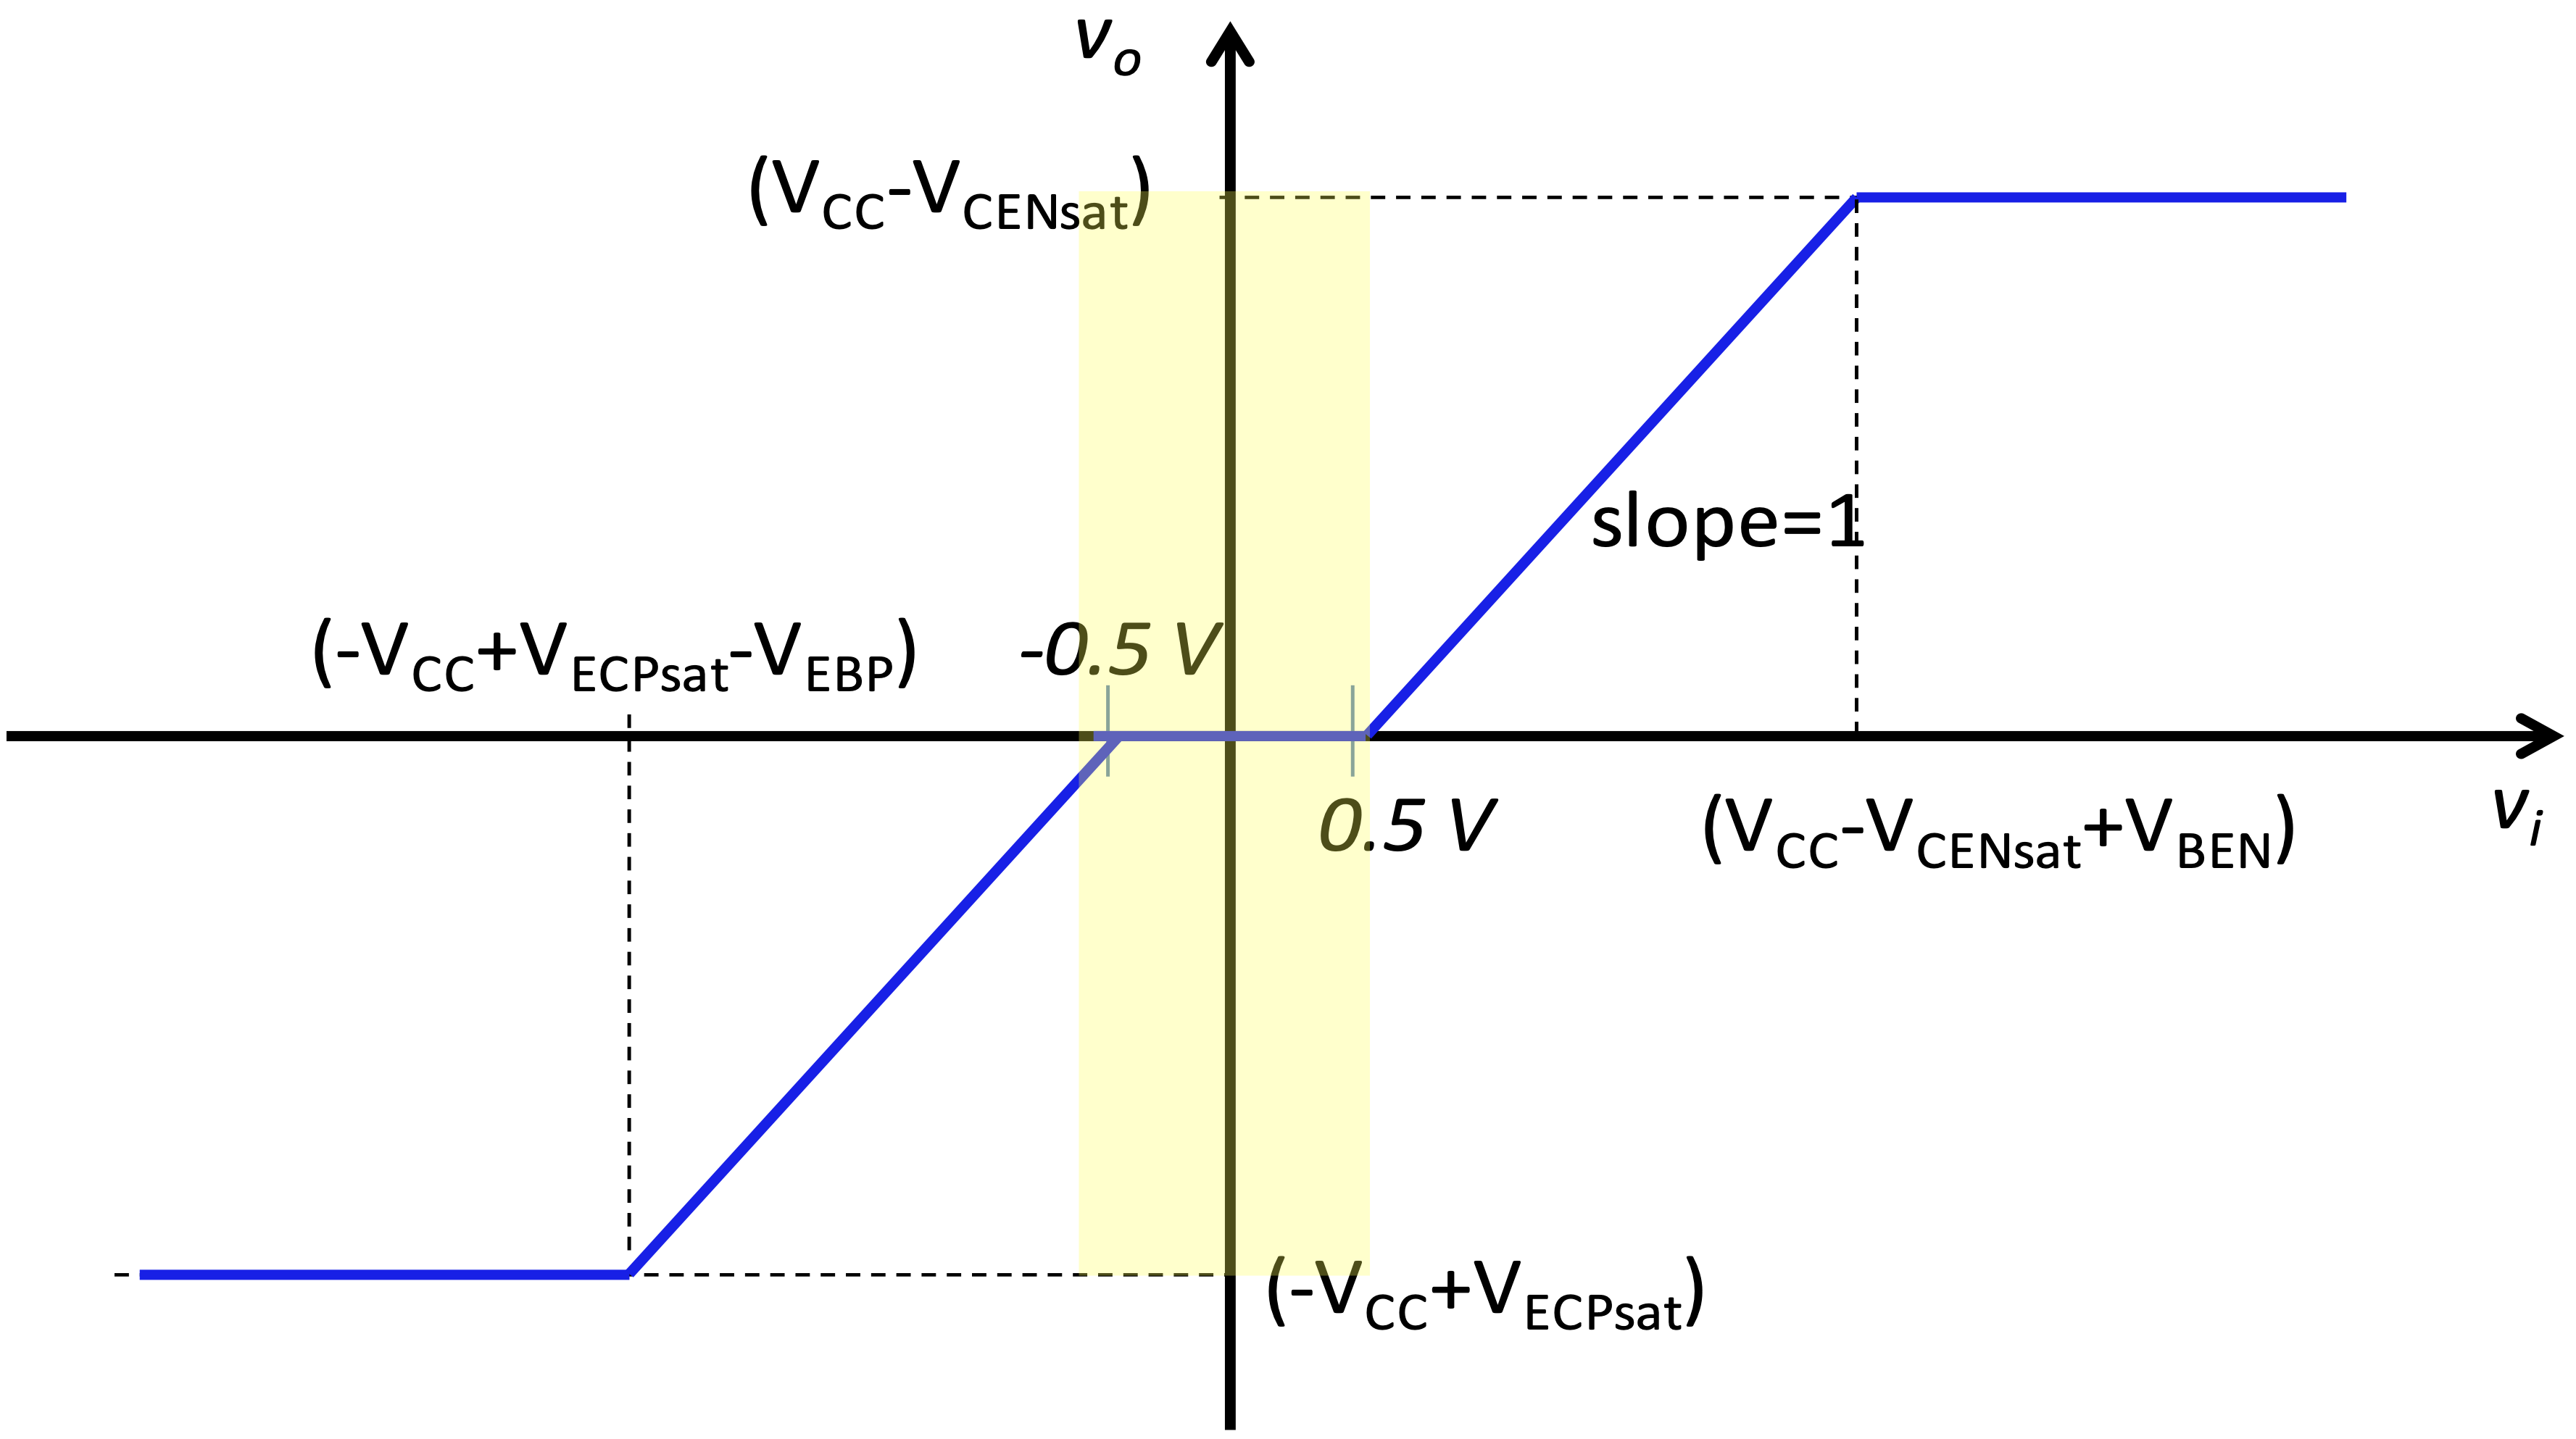
\includegraphics[width=\textwidth]{immagini/class_b_characteristic.png} \\[0.5cm]
		\footnotesize Transfer characteristic of a class B output stage
	\end{minipage}
	\begin{minipage}{0.5\textwidth}
		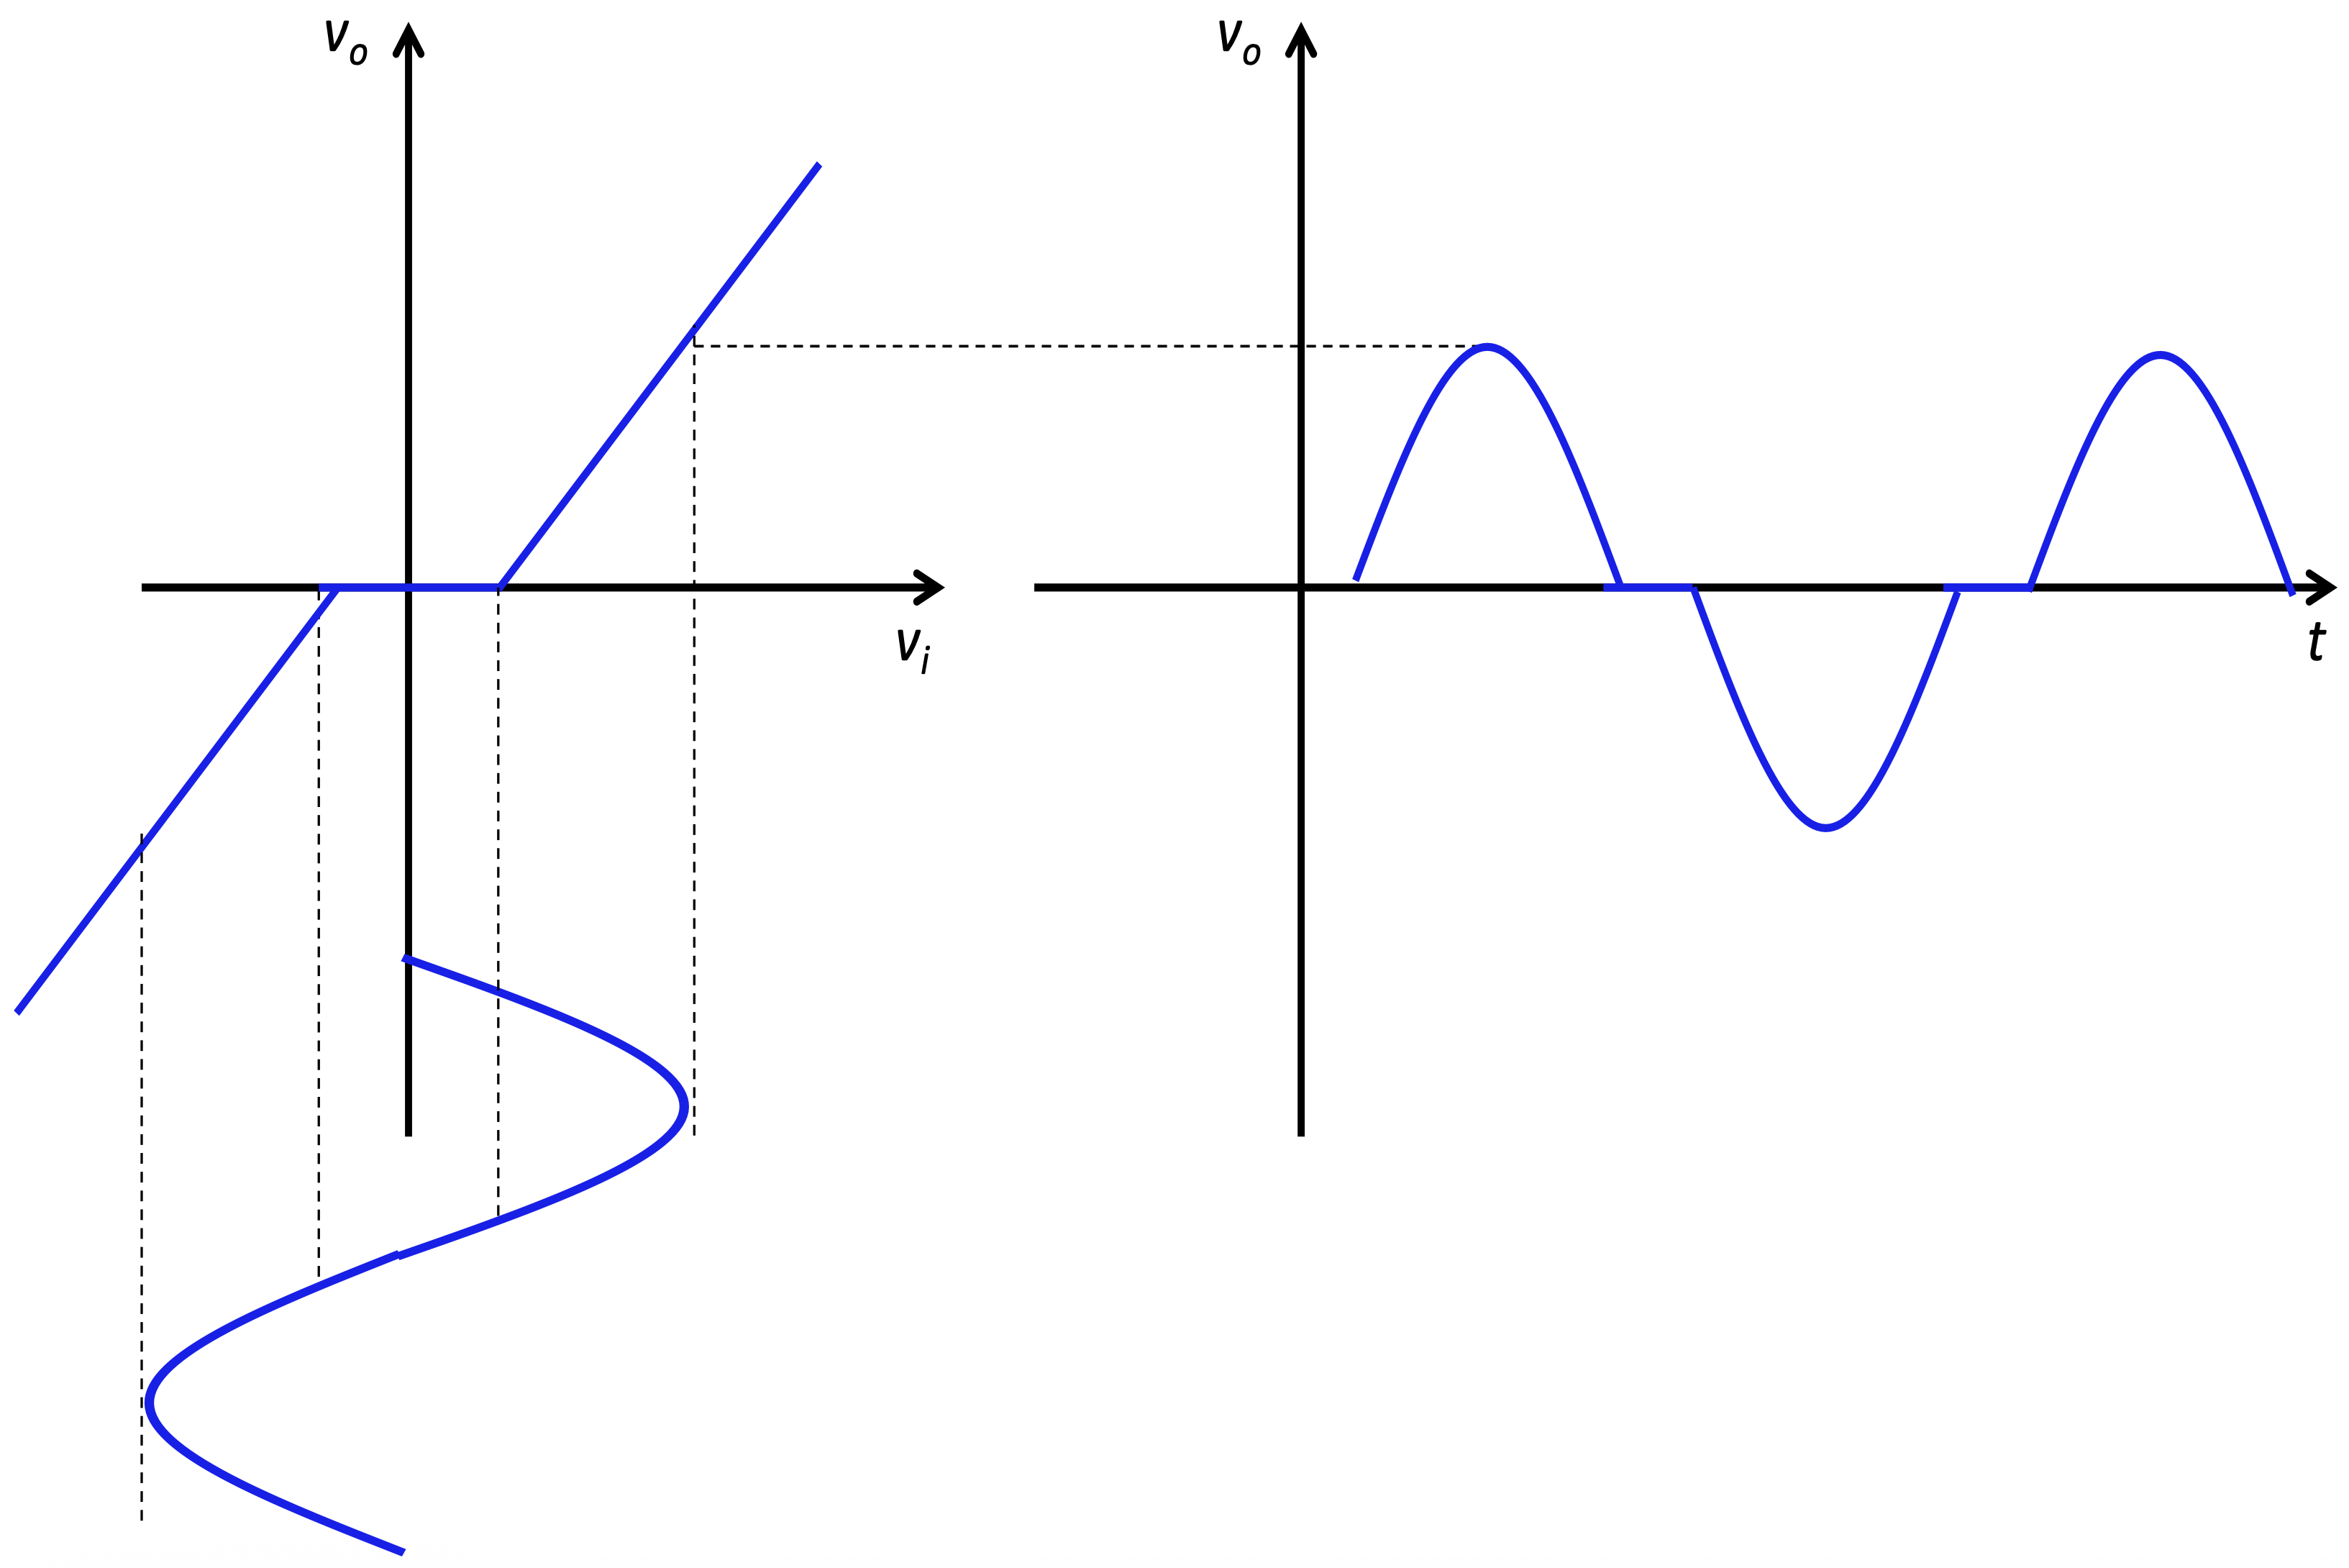
\includegraphics[width=0.8\textwidth]{immagini/class_b_curve.png} \\[0.5cm]
		\footnotesize Example of input and output signals (sinusoidal) of a class B output stage, the crossover distortion is
		clearly visible around the zero crossing of the output signal.
	\end{minipage}
\end{center}

\subsubsection*{Power conversion efficiency}
Can be demonstrated that the maximum power conversion efficiency of a class B output stage is:
\[\eta_{max} = \frac{\pi}{4} = 78.5\%\]

\subsubsection*{Crossover distortion}
The crossover distortion is the distortion that occurs in the output signal when the input signal is around zero, due to the dead
zone between \(-V_{EB,p}\) and \(V_{BE,n}\).

\vspace{10pt}

\begin{center}
	\begin{minipage}{0.5\textwidth}
		\begin{circuitikz}[american, scale=0.8, transform shape]
			\node[npn, anchor=emitter] (Q1) at (0,0) {\(Q_n\)};
			\node[pnp, anchor=collector] (Q2) at (0,-2.5) {\(Q_p\)};
			\draw (Q1.B) -- ++(-0.7,0) -- node[midway] (input) {} ($(Q2.B) + (-0.7,0)$) -- (Q2.B);
	
			\draw (Q1.E) -- node[midway] (output) {} (Q2.E);
			\draw ($(output)$) to[short, -o, i_=\(I_L\), current/distance=0.3] ++(1.5,0) node[right] {$V_{out}$}
				to[R, l=\(R_L\)] ++(0, -2) ++(0,0.4)node[ground] {};
	
			\draw (Q1.C) to[short, -o] ++(0,0) node[above] {$+V_{CC}$};
			\draw (Q2.C) to[short, -o] ++(0,0) node[below] {\(-V_{CC}\)};
		
			\node [xshift=-0.1cm, yshift=-0.2cm] at (Q1.B) (vplus) {$+$};
			\node [xshift=-0.2cm, yshift=-0.2cm] at (Q1.E) (vminus) {$-$};
			\draw (vminus) to node[midway, fill=white, inner sep=3pt] {$V_{BEn}$} (vplus);
	
			\node [xshift=-0.2cm, yshift=0.2cm] at (Q2.E) (vplus) {$+$};
			\node [xshift=-0.1cm, yshift=0.2cm] at (Q2.B) (vminus) {$-$};
			\draw (vminus) to node[midway, fill=white, inner sep=3pt] {$V_{EBp}$} (vplus);
	
			\node[op amp, anchor=out] (opamp) at ($(input) + (-0.5,0)$) {};
			\draw (opamp.out) -- ($(input)$);
			\draw (opamp.+) to[short, -o] ++(-0.5,0) node[left] {$V_{in}$};
			\draw (opamp.-) -- ++(-0.5, 0) -- ++(0,2.1) -- ++(5.62,0) -- ($(output) + (0.7,0)$) node[circ] {};
		\end{circuitikz}
	\end{minipage}
	\begin{minipage}{0.45\textwidth}
		This distortion can be reduced by using an op amp to drive the input signal of the output stage with feedback loop
		to compensate the dead zone as shown on the left.

		\vspace{10pt}
		
		It is important to keep in mind op amps limitations, especially low slew rates can limit the compensation.
	\end{minipage}
\end{center}

\newpage

\subsection{Class AB}
\subsubsection*{Circuit description}
The main idea of the class AB output stage is to reuse the same push-pull configuration of the class B output stage, but with
a bias voltage \(V_{BB}\) applied to the bases of both transistors \(Q_n\) and \(Q_p\) to keep them slightly on even without
input signal. In this way, transistors are always slightly conductive and are able to drive immediately the output signal
without the class B delay and the crossover distortion is virtually eliminated.

\begin{center}
	\begin{minipage}{0.45\textwidth}
		\centering \begin{circuitikz}[american, scale=0.8, transform shape]
			\node[npn, anchor=emitter] (Q1) at (0,0) {\(Q_n\)};
			\node[pnp, anchor=collector] (Q2) at (0,-3) {\(Q_p\)};
			\draw (Q1.B) -- ++(-2.4,0);
			\draw (Q2.B) -- ++(-2.4,0);
			\draw ($(Q1.B)+(-2.4,0)$) to[battery1, v=\(V_{BB}/2\)] ($($(Q2.B) + (-2.4,0)$)!0.5!($(Q1.B) + (-2.4,0)$)$) node (input) {} to[battery1, v=\(V_{BB}/2\)] ($(Q2.B)+(-2.4,0)$);
			\draw ($(input)$) to[short, -o] ++(-1,0) node[left] {$V_{in}$};
	
			\draw (Q1.E) to[short, i=\(I_{N}\)] ($($(Q2.E)!0.5!(Q1.E)$) + (0,0.2)$) -- ++(0,-0.2) node (output) {} -- ++(0,-0.2) to[short, i=\(I_{P}\)] (Q2.E);
			
			\draw ($(output)$) -- ++(0.5,0) to[short, -o, i=\(I_L\)] ++(1.2,0) node[right] {$V_{out}$}
				to[R, l=\(R_L\)] ++(0, -2) ++(0,0.4)node[ground] {};
	
			\draw (Q1.C) to[short, -o] ++(0,0) node[above] {$+V_{CC}$};
			\draw (Q2.C) to[short, -o] ++(0,0) node[below] {\(-V_{CC}\)};
	
			\node [xshift=-0.1cm, yshift=-0.2cm] at (Q1.B) (vplus) {$+$};
			\node [xshift=-0.3cm, yshift=-0.1cm] at (Q1.E) (vminus) {$-$};
			\draw (vminus) to node[midway, fill=white, inner sep=3pt] {$V_{BEn}$} (vplus);
	
			\node [xshift=-0.3cm, yshift=0.1cm] at (Q2.E) (vplus) {$+$};
			\node [xshift=-0.1cm, yshift=0.2cm] at (Q2.B) (vminus) {$-$};
			\draw (vminus) to node[midway, fill=white, inner sep=1pt] {$V_{EBp}$} (vplus);
		\end{circuitikz} \\[0.5cm]
		\footnotesize Circuit of a class AB output stage with bias voltage \(V_{BB}\) applied via two ideal voltage sources.
	\end{minipage}
	\begin{minipage}{0.45\textwidth}
		\centering \begin{circuitikz}[american, scale=0.8, transform shape]
			\ctikzset{diodes/scale=0.8, capacitors/scale=0.8, resistors/scale=0.8}
			
			\node[npn, anchor=emitter] (Q1) at (0,0) {\(Q_n\)};
			\node[pnp, anchor=collector] (Q2) at (0,-3) {\(Q_p\)};
			
			\draw (Q1.C) to[short, -o] ++(0,1) node (vcc) {} node[above] {$+V_{CC}$};
			\draw (Q2.C) to[short, -o] ++(0,-1) node (vss) {}node[below] {\(-V_{CC}\)};

			\draw (Q1.B) -- ++(-1,0) node (base11) {} to[C, l=\(C_1\)] ++(-1.5,0) node (base12) {};
			\draw (Q2.B) -- ++(-1,0) node (base21) {} to[C, l=\(C_2\)] ++(-1.5,0) node (base22) {};
			\draw ($(base11)$) to[D] ($(base11)!0.5!(base21)$) to[D] ($(base21)$);
			\draw ($(base12)$) -- ($(base12)!0.5!(base22)$) node (input) {} -- ($(base22)$);
			\draw ($(base11)$) to[R, l_=\(R_1\)] ++(0.5,+1.5) -| (vcc);
			\draw ($(base21)$) to[R, l=\(R_2\)] ++(0.5,-1.5) -| (vss);
			\draw ($(input)$) to[short, -o] ++(-1,0) node[left] {$V_{in}$};
	
			\draw (Q1.E) to[short, i=\(I_{N}\)] ($($(Q2.E)!0.5!(Q1.E)$) + (0,0.2)$) -- ++(0,-0.2) node (output) {} -- ++(0,-0.2) to[short, i=\(I_{P}\)] (Q2.E);
			
			\draw ($(output)$) -- ++(0.5,0) to[short, -o, i=\(I_L\)] ++(1.2,0) node[right] {$V_{out}$}
				to[R, l=\(R_L\)] ++(0, -2) ++(0,0.4)node[ground] {};
	
			\node [xshift=-0.1cm, yshift=-0.2cm] at (Q1.B) (vplus) {$+$};
			\node [xshift=-0.3cm, yshift=-0.1cm] at (Q1.E) (vminus) {$-$};
			\draw (vminus) to node[midway, fill=white, inner sep=3pt] {$V_{BEn}$} (vplus);
	
			\node [xshift=-0.3cm, yshift=0.1cm] at (Q2.E) (vplus) {$+$};
			\node [xshift=-0.1cm, yshift=0.2cm] at (Q2.B) (vminus) {$-$};
			\draw (vminus) to node[midway, fill=white, inner sep=1pt] {$V_{EBp}$} (vplus);
		\end{circuitikz} \\[0.5cm]
		\footnotesize Circuit of a class AB output stage with bias voltage \(V_{BB}\) applied via two diodes.
	\end{minipage}
\end{center}

In real circuits, the bias voltage \(V_{BB}\) is imposed by using two diodes connected in series between the bases of the
two transistors \(Q_n\) and \(Q_p\) as shown on the right. There are also two capacitors \(C_1\) and \(C_2\) to filter the
bias voltage and two resistors \(R_1\) and \(R_2\) to properly limit the current through the diodes. 

\subsubsection*{Circuit behavior}
\begin{itemize}
	\item[1.] When the input signal passes from zero to positive, the \(Q_n\) transistor starts to conduct more current
	and \(V_{BEn}\) increases. Due to the fact that \(V_{BEn} + V_{EBp} = V_{BB}\), the \(V_{EBp}\) decreases and the
	\(Q_p\) transistor starts to conduct less current until it reaches its minimum conduction.
	\item[2.] Vice versa, when the input signal passes from zero to negative, the \(Q_p\) transistor starts to conduct more
	current and \(V_{EBp}\) increases. The \(V_{BEn}\) decreases and the \(Q_n\) transistor starts to conduct less current
	until it reaches its minimum conduction.
\end{itemize}

If the bias voltage \(V_{BB}\) is big enough, both transistors are slightly conductive at zero input signal and are able
to immediately drive the output signal without delay eliminating the crossover distortion. If the bias voltage \(V_{BB}\)
is too big, it is possible that both transistors remain conductive for the entire input signal period, and the output stage
behaves like a class A output stage with high power dissipation and low efficiency.

\subsubsection*{Quiescent power dissipation}
The problem of this configuration is that when both transistors are on at the same time, there is a direct current flowing from
the positive supply to the negative supply through the transistors, that increases power dissipation and reduces efficiency.

If the \(V_{BB}\) is properly chosen, the quiescent current \(I_{Q}\) is smaller than the load current \(I_L\), so the quiescent
power dissipation is negligible and the efficiency is close to the maximum efficiency of a class B output stage.

\subsubsection*{Current analysis}
From the diode equations applied to the npn and pnp transistors:
\begin{align*}
	I_{N} &= I_S \left( e^{V_{BEn} / V_T} - 1 \right) \approx I_S \left( e^{V_{BEn} / V_T} \right) \quad \rightarrow \quad V_{BEn} = V_T \ln \left( \frac{I_N}{I_S} \right) \\
	I_{P} &= I_S \left( e^{V_{EBp} / V_T} - 1 \right) \approx I_S \left( e^{V_{EBp} / V_T} \right)\quad \rightarrow \quad V_{EBp} = V_T \ln \left( \frac{I_P}{I_S} \right) \\
	I_{Q} &= I_S \left( e^{V_{BB} / 2 V_T} - 1 \right) \approx I_S \left( e^{V_{BB} / 2 V_T} \right) \quad \rightarrow \quad V_{BB} = 2 V_T \ln \left( \frac{I_Q}{I_S} \right)
\end{align*}
\[V_{BEn} + V_{EBp} = V_{BB} \quad \rightarrow \quad V_T \ln \left( \frac{I_N}{I_S} \right) + V_T \ln \left( \frac{I_P}{I_S} \right) = 2 V_T \ln \left( \frac{I_Q}{I_S} \right) \quad \rightarrow \quad I_N \cdot I_P = {I_Q}^2\]

From the Kirchhoff's current law at the output node: \[I_N = I_P + I_L\]

Putting both equations together: \[I_N^2 - I_L \cdot I_N - I_Q^2 = 0\]

By solving the quadratic equation, we can find the current \(I_N\) and \(I_P\):
\[I_N = \frac{I_L}{2} + \sqrt{\left(\frac{I_L}{2}\right)^2 + I_Q^2} \qquad I_P = -\frac{I_L}{2} + \sqrt{\left(\frac{I_L}{2}\right)^2 + I_Q^2}\]
These results show that:
\begin{itemize}
	\item if \(I_L = 0\), then \(I_N = I_P = I_Q\) and both transistors are slightly conductive
	\item if \(I_L\) is big enough, then \(I_N \approx I_L\) and \(I_P \approx 0\) (or vice versa if \(I_L\) is negative), by
	neglecting the \({I_Q}^2\) term in the square root, showing that the output stage behaves like a class B output stage when
	the load current is big enough
\end{itemize}

\subsubsection*{Transfer characteristic}
The transfer characteristic of the class AB output stage with ideal bias voltage \(V_{BB}\) is a perfect straight line with a
slope of 1, no crossover distortion and no voltage offset.
\begin{center}
	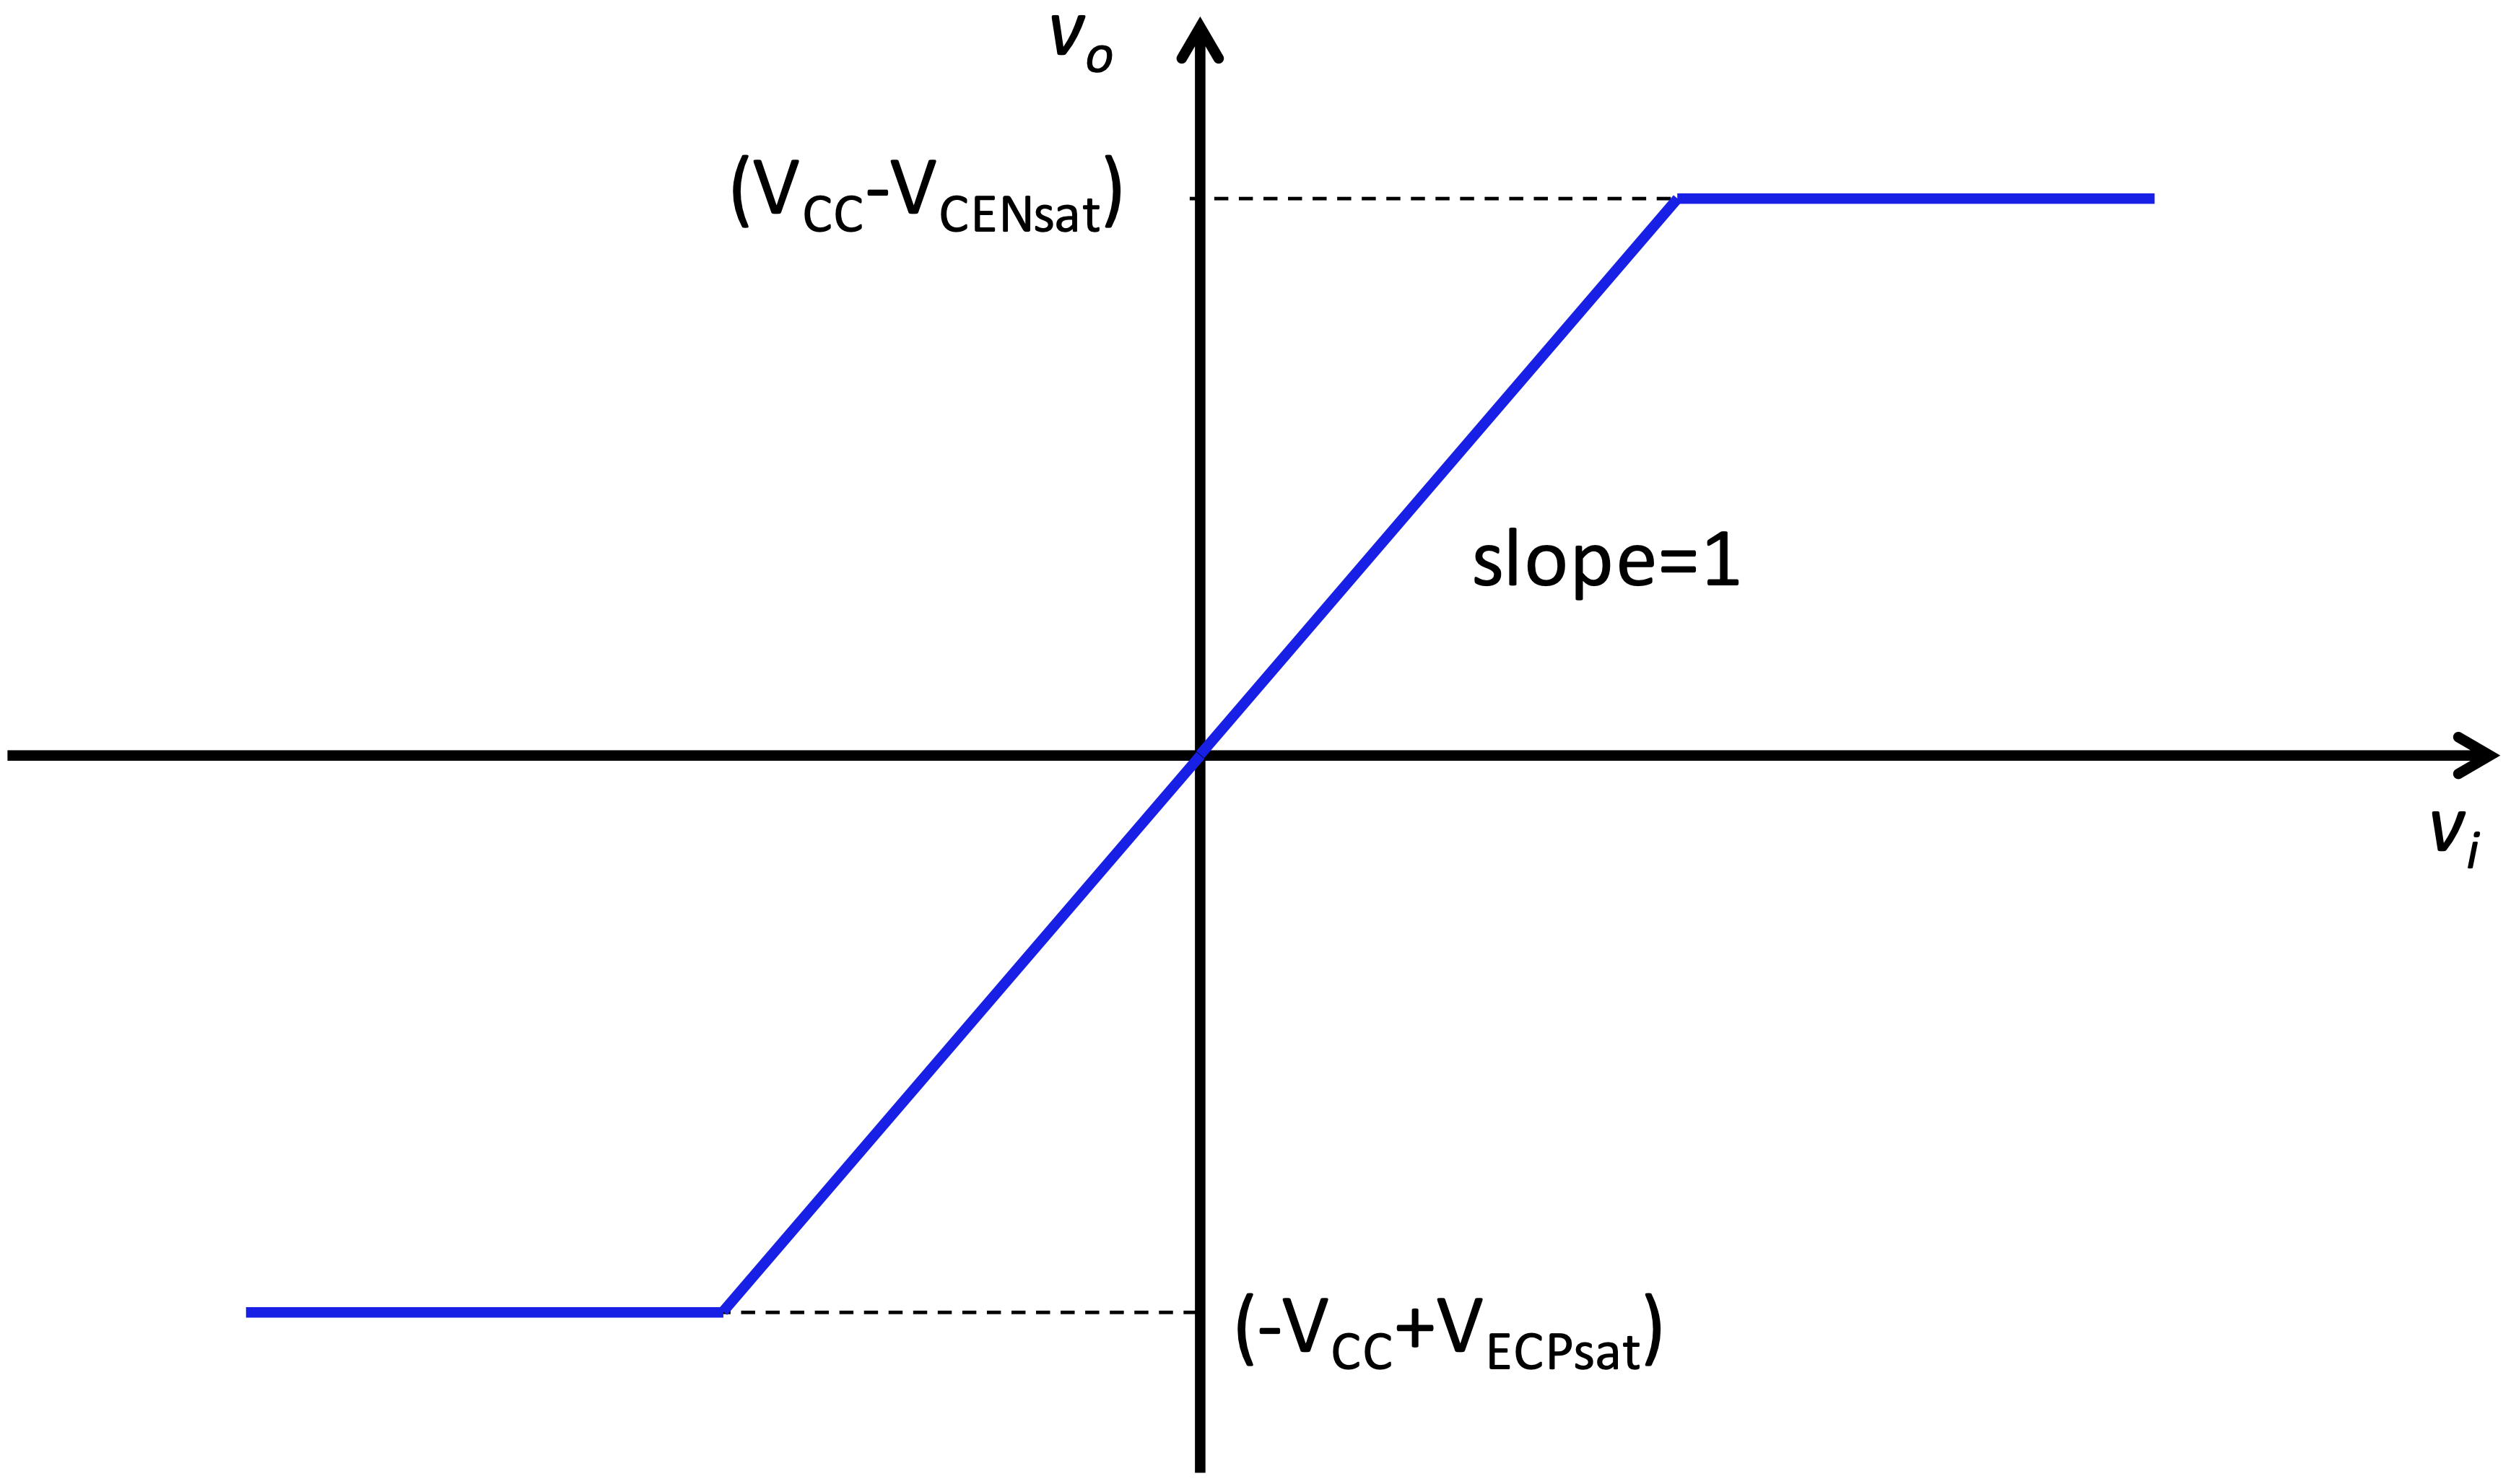
\includegraphics[width=0.5\textwidth]{immagini/class_ab_characteristic.png}
\end{center}

\subsubsection*{Disadvantages}
The main problem of the class AB output stage is to properly set the bias voltage \(V_{BB}\) to eliminate crossover distortion
without increasing too much the quiescent power dissipation. This is a really hard task in real circuits because of the
components tolerances and the temperature variations.

\section{Arduino}
\subsection{Introductions to Arduino and microcontrollers}
\subsubsection*{Microcontrollers}
Microcontrollers are complete computer systems with microprocessor (CPU), clock oscillator, memory and I/O peripherals integrated
on a single chip. Microcontrollers are used to get data from the environment through sensors, process it and control actuators
accordingly. Due to memory and processing power limitations, code for microcontrollers must be written in a very efficient way.

\subsubsection*{Arduino Uno}
Arduino Uno is a microcontroller board based on the ATmega328P microcontroller. It has 14 digital input/output pins and 6 analog
input pins and a 16 MHz quartz crystal. It has an AREF pin for analog reference voltage for ADC and a reset button. It has a USB
connection for programming and a power jack for external power supply. It has a 5V pin (400 mA) and a 3.3V pin (50 mA) connected
to the onboard voltage regulator and a Vin pin connected directly to the input power supply source.

The Atmega328P microcontroller has 32 KB of ISP flash memory for storing code, 2 KB of SRAM for storing variables and 1 KB of
EEPROM for storing non volatile data. It has 23 GPIO (general purpose input/output), 32 general purpose working registers,
6 channel 10-bit ADC, USART, SPI and I2C communication interfaces. It has three timers, internal and external interrupts and
a watchdog timer. It operates at a voltage between 1.8 and 5.5 V.

\subsubsection*{Arduino Mega}
Arduino Mega is a microcontroller board based on the ATmega2560 microcontroller. It has 54 digital input/output pins and 16
analog input pins and a 16 MHz quartz crystal. Due to the higher number of pins, it is used for more complex projects that
require more I/O peripherals.

\subsubsection*{Arduino Due}
Arduino Due is a microcontroller board based on the Atmel SAM3X8E ARM Cortex-M3 CPU. It has 54 digital input/output pins and 12
analog input pins and a 84 MHz quartz crystal. Due to the higher processing power, it is used for more complex projects that
require more processing power and more I/O peripherals. \textbf{It operates at a voltage of 3.3 V and it is not 5V tolerant.}

\subsubsection*{Arduino Nano 33 BLE Sense Rev2}
Arduino Nano 33 BLE Sense Rev2 is a microcontroller board based on the Nordic Semiconductor nRF52840 ARM Cortex-M4 CPU in the
same form factor as the Arduino Nano. It has 14 digital input/output pins and 8 analog input pins and a 64 MHz quartz crystal.
It has a Bluetooth Low Energy (BLE) module and a wide range of sensors, including an accelerometer, a gyroscope, a magnetometer,
a temperature sensor, a humidity sensor, a pressure sensor and a microphone and has an RGB LED. \textbf{It operates at a voltage
of 3.3 V and it is not 5V tolerant.}

\subsubsection*{Other boards}
\begin{itemize}[topsep=-1pt, itemsep=-1pt]
	\item Arduino Uno Wifi Rev2: same form factor as the Uno but with an ATmega4809 microcontroller and a WiFi module with
	integrated TCP/IP protocol stack.
	\item Arduino STAR - Otto: equiped with a powerful ARM processor to control power demanding peripherals like LCD, Audio, Camera, etc.
	\item Arduino Alicepad: board for wearables and clothing
	\item Arduino Nano: same microcontroller as the Uno but in a smaller form factor
	\item Arduino Giga R1 Wifi: board with an ARM Cortex-M7 microcontroller and a WiFi module, designed for high performance
	applications like robotics, AI and machine learning
	\item Arduino Portenta H7: board with an ARM Cortex-M7 microcontroller and a WiFi module, designed for high performance
	applications like robotics, AI and machine learning
	\item Shields: passive boards that can be plugged on top of an Arduino board to extend its functionality
\end{itemize}

\subsection{Programming on Arduino - pin modes, interrupts and timers}
\subsubsection*{Bootloader}
The bootloader is a small program stored in a private section of the flash memory that allows to program the microcontroller
through a simple serial communication. On the board, there is also an USB-to-serial converter that allows to connect the
a computer to the microcontroller via USB and use it as a serial communication interface for programming and debugging.

Usually the bootloader is pre-flashed on the microcontroller by the manufacturer. If the bootloader is not present or needs
to be updated, it must be flashed on the microcontroller via the SPI communication pins (MOSI, MISO, SCK) connected to an
external programmer.

\subsubsection*{Program structure}
An arduino program is called a sketch and it is written in C/C++. It has two main functions:
\begin{itemize}
	\item \texttt{setup()}: executed only once, when the microcontroller is powered on or reset; it is used to initialize
	variables, object instances of peripherals, pin modes and other settings
	\item \texttt{loop()}: executed repeatedly after the \texttt{setup()} function; it is used to implement the main logic
	of the program
\end{itemize}

\noindent
Considerations about the program structure:
\begin{itemize}
	\item global variables are preferrred to local variables, because they are stored in the flash memory and do not consume
	SRAM, which is a very limited resource on microcontrollers
\end{itemize}

\subsubsection*{Pin modes and pin functions}
Arduino pins can be configured in different modes and can perform different functions.
\begin{itemize}
	\item digital output: pin configured as a digital output, used to write digital signals (LOW or HIGH) through
	\texttt{digitalWrite(PIN, [HIGH,LOW])} function
	\item digital input: pin configured as a digital input, used to read digital signals (HIGH or LOW) through
	\texttt{digitalRead(PIN)} function
	\item analog output: pin configured as a digital PWM output, used to write PWM signals with custom duty cycle in
	range 0-255 through \texttt{analogWrite(PIN, value)} function, PWM frequency can vary depending on board and pin used
	\item analog input: pin configured as an analog input, used to read analog signals through the ADC and get
	a digital value in range 0-1023 (for 10-bit ADC) through \texttt{analogRead(PIN)} function
\end{itemize}

\noindent
To configure how the pin behaves, the \texttt{pinMode(PIN, MODE)} function is used in the \texttt{setup()} function, where
\texttt{MODE} can be one of the following:
\begin{itemize}
	\item \texttt{OUTPUT}: configures the pin as a digital output
	\item \texttt{INPUT}: configures the pin as an analog/digital input
	\item \texttt{INPUT\_PULLUP}: configures the pin as a digital input with an internal pull-up resistor, in this mode the pin
	is connected to \(V_{CC}\) through a \(\approx 22 \; k\Omega\) pull-up resistor, so the pin reads HIGH when it is not connected to
	ground and LOW when it is connected to ground.
\end{itemize}

\subsubsection*{Analog readings and ADC configuration}
The resolution of the ADC can be changed by calling the \texttt{analogReadResolution(bits)} function in the \texttt{setup()}
function. By default, the resolution is 10 bits (0-1023), but it can be increased to 12 bits (0-4095) on some boards like the
Arduino Due and the Arduino Nano 33 BLE Sense Rev2.

It is possible to set an external high-voltage reference for the ADC by connecting that reference voltage to the AREF pin and
calling the \texttt{analogReference(EXTERNAL)} function in the \texttt{setup()} function. By default, the reference voltage is
the supply voltage (5V or 3.3V depending on the board).

The resolution step of the ADC can be calculated as follows:
\[\text{ADC step} = \frac{V_{REF}}{2^{\text{bits}}} \qquad \text{by default} \begin{array}{l l}
	\text{Arduino Uno: } & \displaystyle \text{ADC step} = \frac{5 \; V}{2^{10 \; \text{bits}}} = 4.88 \; mV \\[7pt]
	\text{Arduino Nano 33 BLE: } & \displaystyle \text{ADC step} = \frac{3.3 \; V}{2^{12 \; \text{bits}}} = 0.806 \; mV
\end{array}\]

\subsubsection*{The \texttt{millis}, \texttt{micros} and \texttt{delay} functions}
These three functions are used to manage time in Arduino sketches and use internal timers of the microcontroller.
\begin{itemize}
	\item \texttt{millis()}: returns the number of milliseconds since the microcontroller was powered on or reset;
	it returns an unsigned 32-bit integer, so it overflows after approximately 50 days
	\item \texttt{micros()}: returns the number of microseconds since the microcontroller was powered on or reset;
	it returns an unsigned 32-bit integer, so it overflows after approximately 70 minutes; due to limited clock speed
	on some boards, the resolution of this function can be 4 microseconds (16 MHz clock)
	\item \texttt{delay(ms)}: blocks the execution of the program for a specified number of milliseconds
\end{itemize}

\noindent
Use of the \texttt{millis()} and \texttt{micros()} functions is preferred to the use of the \texttt{delay()} function,
because it does not block the execution of the program and allows to implement non-blocking delays and timeouts, which
are essential for implementing real-time applications.

\subsubsection*{Interrupts}
An interrupt is a signal that can be generated by an external event (for example a button press) or by an internal event
(for example a timer overflow) that interrupts the normal execution of the program and executes a special function called
interrupt service routine (ISR). Interrupts are used to handle events that require immediate attention and cannot be handled
in the loop function of the program, for example user interactions.

\noindent
Interrupt service routines has the following characteristics:
\begin{itemize}
	\item they must be as short and fast as possible
	\item only one interrupt can be executed at a time so if multiple interrupts are generated at the same time, they are
	executed in order of priority
	\item only \texttt{delayMicroseconds()} function works inside an ISR, while \texttt{delay()} and \texttt{millis()}
	functions do not work because they rely on interrupts to update the internal timers
	\item they do not accept parameters and do not return values, so they must use \texttt{volatile} global variables to
	communicate with the main program. The keyword \texttt{volatile} is used to prevent the compiler from optimizing operations
	on those variables and causing race conditions.
\end{itemize}

\noindent
To attach an interrupt to a pin, the \texttt{attachInterrupt(digitalPinToInterrupt(PIN), ISR, MODE)} function is used in the
\texttt{setup()} function where:
\begin{itemize}
	\item \texttt{PIN} is the pin number to which the interrupt is attached (only supported pins can be used)
	\item \texttt{ISR} is the name of the interrupt service routine function
	\item \texttt{MODE} is the condition that triggers the interrupt and can be one of the following:
	\begin{itemize}[topsep=-1pt]
		\item \texttt{RISING}: triggers the interrupt when the pin goes from LOW to HIGH
		\item \texttt{FALLING}: triggers the interrupt when the pin goes from HIGH to LOW
		\item \texttt{CHANGE}: triggers the interrupt when the pin changes state (from LOW to HIGH or vice versa)
		\item \texttt{LOW}: triggers the interrupt when the pin is LOW (only for some boards)
		\item \texttt{HIGH}: triggers the interrupt when the pin is HIGH (only for some boards)
	\end{itemize}
\end{itemize}

\subsubsection*{Switch-case, \texttt{break} \texttt{continue} statements}
Switch-case statements are used to execute different blocks of code based on the value of a variable. They are more efficient
than if-else statements when there are many cases to handle, because they use a jump table instead of evaluating multiple
conditions.

The \texttt{break} and \texttt{continue} statements are used to control the flow of loops and switch-case statements. The
\texttt{break} statement is used to exit a loop or a switch-case statement, while the \texttt{continue} statement is used
to skip the current iteration of a loop and continue with the next iteration.

\newpage

\subsection{Simple circuits with Arduino}
\subsubsection*{Drive a LED directly connected to an Arduino pin}
To correctly bias a LED, a current limiting resistor must be used in series with the LED. The value of the resistor can be
calculated using Ohm's law as follows.

\begin{center}
	\begin{minipage}{0.5\textwidth}
		\centering \begin{circuitikz}[american, scale=0.8, transform shape]
			\circuitikzset{diodes/scale=0.8}
			\draw (0,0) node[left] {\(\begin{array}{c} V_{CC} \\ \text{\footnotesize Arduino pin} \end{array}\)} to[short, o-] ++(0.5,0) to[R, l=$R$] ++(2,0) to[leD, l=$LED$] ++(2, 0) node[ground] {};
		\end{circuitikz}
	\end{minipage}
	\begin{minipage}{0.45\textwidth}
		\[R = \frac{V_R}{I_R} = \frac{V_{CC} - V_{LED}}{I_{LED}}\]
	\end{minipage}
\end{center}

\subsubsection*{Drive high current into a LED with a BJT}
Arduino pins can source or sink a limited amount of current (4mA for Nano 33 BLE Sense Rev2). If a higher current is needed,
a BJT can be used as a switch to drive the LED. The base of the BJT is connected to the Arduino pin through a current limiting
resistor, the collector is connected to the LED with a current limiting resistor in series and the emitter is connected to ground.
The transistor is used as a switch in saturation regime, so the voltage drop across the collector-emitter junction is negligible
and the current through the LED is determined by the current limiting resistor and the supply voltage.

\begin{center}
	\begin{minipage}{0.5\textwidth}
		\centering \begin{circuitikz}[american, scale=0.8, transform shape]
			\circuitikzset{diodes/scale=0.8}
			\circuitikzset{transistors/scale=1.4}
			\draw (0,0) node[left] {\(V_{CC}\)} to[short, o-] ++(0.5,0) to[R, l=$R_{LED}$] ++(2,0) to[leD, l=$LED$] ++(2, 0) node[npn, anchor=collector, rotate=90] (npn) {};
			\draw (npn.emitter) -- ++(0.5, 0) node[ground] {};
			\draw (npn.base) to[R, l=$R_B$] ++(0,-1.5) to[short, -o] ++(0, -0.5) node[left] {\(\begin{array}{c} V_{CC} \\ \text{\footnotesize Arduino pin} \end{array}\)};

			\node [xshift=0.2cm, yshift=0.1cm] at (npn.B) (vplus) {$+$};
			\node [xshift=-0.2cm, yshift=-0.2cm] at (npn.E) (vminus) {$-$};
			\draw[-{Latex}] (vminus) to[out=-90, in=10] node[pos=0.3, fill=white, inner sep=1pt] {$V_{BE}$} (vplus);
		\end{circuitikz}
	\end{minipage}
	\begin{minipage}{0.45\textwidth}
		\[R_{LED} = \frac{V_{R_{LED}}}{I_{R_{LED}}} = \frac{V_{CC} - V_{LED}}{I_{LED}}\]
		\vspace{5pt}
		\[R_B = \frac{V_{R_B}}{I_{R_B}} = \frac{V_{CC} - V_{BE}}{I_B}\]
	\end{minipage}
\end{center}

\subsubsection*{Dimming an LED / RGB-LED with \texttt{analogWrite()} and PWM signal}
By using the \texttt{analogWrite(PIN, value)} function, it is possible to generate a PWM signal on a digital pin (with PWM support)
and control the brightness of a LED by changing the duty cycle of the PWM signal. Value can be in range 0-255, where 0 means 0\% duty
cycle (LED off) and 255 means 100\% duty cycle (LED fully on).

On the Arduino Nano 33 BLE Sense Rev2, there is a built-in RGB LED controlled by three virtual pins (\texttt{LED\_R},
\texttt{LED\_G}, \texttt{LED\_B}). By using the \texttt{analogWrite()} function on these pins, it is possible to control
the brightness of each color and create different colors by mixing the three primary colors.

\subsubsection*{Read a button state with \texttt{digitalRead()}, pull-up resistors and debouncing}
A button is a simple switch that can be used to connect a pin to ground when pressed. The main problem is that when the button
is not pressed, the pin is left floating and can read random values. To solve this problem, a pull-up resistor should be used
to connect the pin to \(V_{CC}\). In this way, when the button is not pressed, the pin reads HIGH and when the button is pressed,
the pin reads LOW.

\begin{center}
	\begin{circuitikz}[american, scale=0.8, transform shape]
		\draw (0,0) node[left] {\(V_{CC}\)} to[short, o-] ++(0.5,0) to[R, l=$R_{PU}$] ++(2,0) to[push button, l=\texttt{button}] ++(2, 0) node[ground] {};
		\draw (2.5, 0) to[short, -o] ++(0, 1) node[above] {\texttt{digital pin}};
	\end{circuitikz}
\end{center}

To choose the value of the pull-up resistor, it is necessary to consider the current that flows through the resistor when the
button is pressed (when the button is not pressed, the current is negligible because the pin is in high impedance state). The
suggested current is in the order of 0.1 - 0.2 mA, so the value of the pull-up resistor can be calculated as follows.
\[I_{R_{PU}} = \frac{V_{CC}}{R_{PU}} \qquad \text{common values are}: \begin{array}{l}
	20-22 \; k\Omega \text{ for } 5 \; V \text{ boards} \\[7pt]
	10-12 \; k\Omega \text{ for } 3.3 \; V \text{ boards}
\end{array}\]

On some boards like the Arduino Uno, there are internal pull-up resistors of 20 k\(\Omega\) that can be enabled by configuring
the pin mode as \texttt{INPUT\_PULLUP}. In this way the button can be connected directly between the pin and ground, without
the need of an external pull-up resistor.

Usually, when a button is pressed, the transition from HIGH to LOW is not clean and immediate, but there are some oscillations
called bouncing due to mechanical switch contacts oscillations. To solve this problem, a simple software debouncing technique
can be used, which consists in waiting for a short time (10 and 50 ms) between two consecutive readings of the button state.

Alternatively, a pull-down resistor can be used between the pin and ground and the button will be connected between the pin
and \(V_{CC}\). The button behaviour becomes active-HIGH, meaning the state will be HIGH when the button is pressed and LOW
when the button is not pressed. 

\subsubsection*{Read a potentiometer value with \texttt{analogRead()}}
It is possible to read the voltage value of a potentiometer wiper terminal by connecting it to an analog input pin. The voltage
at the wiper terminal will be in range \([0, V_{CC}]\) and can be read by an analog pin using the \texttt{analogRead()} function.
The value returned is in range \([0, \;1023]\) for a 10-bit ADC or in range \([0, \; 4095]\) for a 12-bit ADC and is linearly
proportional to the wiper voltage.

In some applications, it is necessary to scale the value read from the potentiometer to a different range (for example \([0, \; 255]\)
to control the brightness of an LED). To do this, it is possible to use the \texttt{map(x, in\_min, in\_max, out\_min, out\_max)}
function to map the value \(x\) from the input range \([\texttt{in\_min}, \; \texttt{in\_max}]\) to the output range
\([\texttt{out\_min}, \; \texttt{out\_max}]\) as follows:
\[\texttt{map(x, in\_min, in\_max, out\_min, out\_max)} \; = \; \frac{(\texttt{x} - \texttt{in\_min}) \times (\texttt{out\_max} - \texttt{out\_min})}{\texttt{in\_max} - \texttt{in\_min}} + \texttt{out\_min}\]

\subsubsection*{Read analog sensors with \texttt{analogRead()}}
Sometimes the output voltage of an analog sensor has a smaller range \([0, V_{sensor,max} < V_{CC}]\). To correctly read the
sensor value, it is necessary to scale the sensor output voltage to the full range of the ADC. This can be done in different ways:
\begin{itemize}
	\item using the \texttt{map()} function to map the value read from the sensor, but does not increase the resolution of the ADC
	because is done after the ADC conversion
	\item using an external op-amp to amplify the sensor output voltage to the full range of the ADC; attention must be paid to
	not exceed the maximum input voltage of the ADC
	\item using the AREF pin to set the reference voltage of the ADC to the maximum sensor output voltage, so the ADC will
	automatically scale the sensor output voltage to the full range of the ADC (this one is the preferred solution)
\end{itemize}

\subsubsection*{Read temperature with analog TMP36 temperature sensor}
TMP36 is an analog temperature sensor that outputs a voltage linearly proportional to the temperature. The output voltage has
a 0.5 V offset (0.5 V correspond to 0\(^\circ C\)) and a slope of 10 mV/\(^\circ C\).
To read the temperature with an Arduino, the output voltage of the TMP36 sensor can be read with an analog input pin and
converted into temperature using the following mapping formula considering (155 correspond to 0.5 V and 330 is the temperature
range for 3.3 V power supply).
\[T = \frac{V_{out} - 0.5 \; V}{10 \; mV/^\circ C} = (V_{out} - 0.5 \; V) \times 100 \; ^\circ C/V \quad \rightarrow \quad \texttt{temperature = (value-155) * 330 / 1023;}\]

\subsubsection*{Read humidity with analog HIH5030 humidity sensor}
HIH5030 is an analog humidity sensor that outputs a voltage linearly proportional to the relative humidity. The output voltage
can be read with an analog input pin and converted into relative humidity using one of the following mapping formulas (from the datasheet).
\[\begin{array}{c}
	RH = (V_{out} / V_{CC} - 0.1515) / 0.00636 \\[5pt]
	V_{out} = \text{measured\_value} \cdot V_{CC} / 1023
\end{array} \quad \rightarrow \quad \texttt{humidity = (value / 1023 - 0.1515) / 0.00636;}\]

\newpage

\subsection{Asynchronous Serial Protocol}
\subsubsection*{Introduction to asynchronous serial protocols}
Asyncronous Serial Protocol is a family of communication protocols that allow to exchange data between the microcontroller
and other devices using a serial communication interface. It has the following characteristics:
\begin{itemize}
	\item asynchronous: the data is transmitted without a clock signal, so the sender and the receiver must agree before the
	communication on the baud rate (bits per second) and the format of the data (start and stop bits, parity bit, etc.)
	\item serial: the data is transmitted serially, one bit at a time, not in parallel
\end{itemize}

\subsubsection*{UART - Universal Asynchronous Receiver-Transmitter protocol}
The UART protocol is the asynchronous serial protocol used for the communication between an Arduino board and other device.
It is a full-duplex protocol that uses two lines for communication: TX (transmit) and RX (receive). The TX line of one device is connected to the RX line
of the other device and vice versa. In idle state, lines are HIGH. The communication has the following format:
\begin{itemize}
	\item start bit: 1 bit LOW, indicates the start of a data frame
	\item data bits: bits transmitted in little endian order (least significant bit first)
	\item stop bit: 1 bit HIGH, indicate the end of a data frame
\end{itemize}

\noindent

\subsubsection*{Serial communication with Arduino}
In Arduino boards, the UART protocol is implemented on the digital pins 0 (RX) and 1 (TX) for communication with other devices
and on the USB port for communication with the computer via the USB-to-serial converter. The Arduino IDE provides a built-in
Serial Monitor or a Serial plotter to visualize the data sent from the Arduino to the computer through the USB port and to send
data from the computer to the Arduino.

In Arduino sketches, the UART protocol is accessed through the \texttt{Serial} class, which provides the following functions:
\begin{itemize}
	\item \texttt{Serial.begin(baud\_rate)}: initializes the serial communication with the specified baud rate, usually used
	in the \texttt{setup()} function, common baud rates are 300, 600, 1200, 2400, 4800, 9600, 14400, 19200, 28800, 38400, 57600,
	115200 bps 
	\item \texttt{Serial.print(data)}: sends data to the serial port as human-readable ASCII text
	\item \texttt{Serial.println(data)}: same as \texttt{Serial.print()}, plus append a newline character at the end
	\item \texttt{Serial.available()}: returns if there is data available to read from the serial port
	\item \texttt{Serial.read()}: reads a byte of data from the serial port; returns -1 if no data is available
\end{itemize}

\newpage

\subsection{Serial Peripheral Interface - SPI}
\subsubsection*{Introduction to SPI protocol}
Serial Peripheral Interface (SPI) is a synchronous serial communication protocol that uses a master-slave architecture to exchange
data between a single controller device (master) and one or more controlled peripheral devices (slaves).

\subsubsection*{SPI connection lines}
The SPI protocol uses at least four lines for communication:
\begin{itemize}
	\item SCLK (Serial Clock): generated by the master to synchronize the communication
	\item CIPO (Controller In Peripheral Out): transmit data from the peripheral to the controller (ex MISO)
	\item COPI (Controller Out Peripheral In): transmit data from the controller to the peripheral (ex MOSI)
	\item CS (Chip Select): line used to select a specific peripheral device (active LOW)
\end{itemize}
SCLK, CIPO and COPI lines are shared between all devices on the SPI bus, while each peripheral device has its own CS line
connected to the master.

\subsubsection*{SPI communication process}
The SPI communication woks as follows:
\begin{itemize}
	\item the master selects the slave device by pulling its CS line LOW
	\item the master generates the clock signal on the SCLK line
	\item on each clock edge, the master and the slave exchange one bit of data on the CIPO and COPI lines
	\item after the communication is finished, the master stops the clock signal and pulls the CS line HIGH
\end{itemize}

\subsection{Libraries in Arduino}
\subsubsection*{Introduction to Arduino/C/C++ libraries}
A library is a collection of functions and declarations that provide extra functionality which can be used in multiple
arduino sketches without the need to write the code from scratch. Libraries are organized in:
\begin{itemize}
	\item header file (.h): contains the declarations of the functions and variables provided by the library
	\item source file (.cpp): contains the implementation of the functions declared in the header file
\end{itemize}

\subsubsection*{Classes and objects in Arduino libraries}
Usually libraries contain classes that are user-defined data structures that encapsulate data and functions and are used to
manage peripherals and sensors or software tools in a more organized way. Classes are defined in the header file and implemented
in the source file. Classes are instantiated in the arduino sketch to create objects of that class, which can be used to call
the functions provided by the library and manage the peripheral or sensor associated with that class.
Classes have the following components:
\begin{itemize}
	\item class constructor: a special function that is called when an object of the class is instantiated, it initializes
	the object and its variables
	\item public functions: functions that can be called from outside the class, they are used to provide the functionality
	of the class
	\item private variables: variables that can only be accessed from within the class, they are used to store the state of
	the object and other internal data
	\item private functions: functions that can only be called from within the class, they are used to implement internal
	functionality of the class that is not exposed to the user, conventionally they are prefixed with an underscore to indicate
	that they are private
\end{itemize}

\newpage

\subsubsection*{Example of header file with class definition}
\begin{lstlisting}[language=C++]
	#ifndef CLASS_NAME_H // include guard to prevent multiple inclusions
	#define CLASS_NAME_H // of the header file

	#include <Arduino.h> // Arduino library with Arduino-specific functions and types

	class ClassName {
		public:
			ClassName(); // constructor
			void function1(); // public function or procedure
			int function2(int param); // public function with parameter and return value

		private:
			int variable1; // private variable
			float variable2; // private variable
			void privateFunction(); // private function
	};

	#endif // CLASS_NAME_H
\end{lstlisting}

\subsubsection*{Example of source file with class implementation}
\begin{lstlisting}[language=C++]
	#include <Arduino.h> // Arduino library with Arduino-specific functions and types
	#include "ClassName.h" // header file with class definition

	ClassName::ClassName() {
		// constructor implementation
	}

	void ClassName::function1() {
		// function implementation
	}

	int ClassName::function2(int param) {
		// function implementation
	}

	void ClassName::privateFunction() {
		// private function implementation
	}
\end{lstlisting}

\subsubsection*{Library file organisation and syntax highlighting}
To use a user-made library in an Arduino sketch, the library files (header and source files) must be placed in a specific folder
with the same name as the library in the Arduino libraries folder.

Usually, user-defined libraries contains symbols and variables that are not recognized by the Arduino IDE as keywords. To enable
syntax highlighting for those symbols, it is possible to add a keyword file in the library folder with the same name as the library
and the extension .txt that contains the list of keywords to be highlighted, for example:
\begin{lstlisting}
	--- inside ClassName.txt file ---
	ClassName    KEYWORD1
	function1    KEYWORD2
	function2    KEYWORD2
\end{lstlisting}

\newpage

\subsection{I\texorpdfstring{\textsuperscript{2}}{2}C Protocol}
\subsubsection*{Introduction to I\texorpdfstring{\textsuperscript{2}}{2}C Protocol}
The I\(^2\)C (Inter-Integrated Circuit) is a synchronous serial communication protocol that uses a master-slave architecture
where multiple devices can communicate over a common bus made of only two lines.

\subsubsection*{I\texorpdfstring{\textsuperscript{2}}{2}C connection lines}
The I\(^2\)C protocol uses two lines for communication:
\begin{itemize}
	\item SDA (Serial Data): line used to transmit data between devices
	\item SCL (Serial Clock): line used to synchronize the communication, is generated by the master device and can be forced
	low by the slave devices to pause the communication when they are not ready to receive or transmit data
\end{itemize}
NOTE: SDA line can change state only when SCL is LOW, exept for the start and stop conditions.

\subsubsection*{I\texorpdfstring{\textsuperscript{2}}{2}C communication process}
Every device on the I\(^2\)C bus has a unique 7-bit address that is used to identify the device during communication. If the
datasheet of the device specify an 8-bit address, a right shift of 1 bit must be applied (the least significant bit is eliminated).
The communication process works as follows:
\begin{itemize}
	\item the master device initiates the communication by sending a start condition (SCL keeps HIGH while SDA goes from
	HIGH to LOW) and starts generating the clock signal on the SCL line
	\item the master device sends the 7-bit address of the slave device it wants to communicate with, followed by a R/W bit
	(0 for write, 1 for read) to indicate if it wants to send or receive data from the slave and in the end the master
	releases the SDA line to allow the slave device to respond
	\item the slave device with the matching address responds with an ACK bit (0) if it is ready to communicate, otherwise
	it responds with a NACK bit (1) if it is not ready
	\item if the slave device ACKs the address, the master and the slave can exchange data bytes, according to the R/W bit
	sent by the master; after each byte of data, the receiver must send an ACK bit (0) or a NACK bit (1) to indicate whether
	transmission was successful or not
	\item after the communication is finished, the master sends a stop condition (SCL keeps HIGH while SDA goes from LOW to HIGH)
	and stops generating the clock signal on the SCL line
\end{itemize}

\subsubsection*{\texorpdfstring{\texttt{Wire.h}}{Wire} library to handle I\texorpdfstring{\textsuperscript{2}}{2}C communications}
In Arduino, the I\(^2\)C protocol is implemented through the \texttt{Wire} library, which provides functions to easily manage
I\(^2\)C communication. The library provides the following functions:
\begin{itemize}
	\item \texttt{Wire.begin()}: initializes the I\(^2\)C communication, must be called in the \texttt{setup()} function before
	using any other function of the library;
	\item \texttt{Wire.beginTransmission(address)}: initiates a transmission to the slave device with the specified address
	\item \texttt{Wire.write(data)}: enqueues a byte of data to the buffer for the slave device
	\item \texttt{Wire.endTransmission()} sends the bytes equeued in the buffer and ends the transmission
	\item \texttt{Wire.requestFrom(address, quantity)}: requests a specified quantity of bytes from the slave device with the
	specified address; returns the number of bytes received from the slave device
	\item \texttt{Wire.read()}: reads a byte of data received from the slave device; returns -1 if no data is available
\end{itemize}
The I\(^2\)C buffer is limited to 32 bytes, so if more data needs to be sent or received, it is necessary to split the data
into multiple transmissions.

There can be multiple Wire buses on the same Arduino board, for example on the Arduino Nano 33 BLE Sense Rev2 there is a second
I\(^2\)C bus connected by \texttt{Wire1.h} library, specifically designed to manage the built-in sensors on the board.

\subsubsection*{Using DS1621 digital temperature sensor with I\texorpdfstring{\textsuperscript{2}}{2}C communication}
The DS1621 is a digital temperature sensor that communicates over the I\(^2\)C bus. It has a 7-bit address that can be partially
configured using external pins of the sensor obtaining the 7-bit address in the following format: ``\texttt{1 0 0 1 A2 A1 A0}''.
I\(^2\)C commands for the DS1621 sensor are as follows:
\begin{itemize}
	\item \texttt{0xAC}: write the next byte into the configuration register of the sensor
	\item \texttt{0x02}: enable the continuous conversion mode of the sensor (temperature is continuously measured and updated in the sensor registers)
	\item \texttt{0xEE}: start a single temperature conversion (temperature is measured once and updated in the sensor registers)
	\item \texttt{0xAA}: read the temperature value from the sensor registers
\end{itemize}

Temperature values are represented in two bytes: the first byte contains the integer part of the temperature in two's complement
format, while the second byte contains the fractional part of the temperature in increments of 0.5\(^\circ C\) (0 for +0\(^\circ C\)
and 128 for +0.5\(^\circ C\)).

The following sketch shows how to use the \texttt{Wire} library to read the temperature value from the DS1621 sensor and print
it to the serial monitor.

\begin{lstlisting}[language=c++]
	#include <Wire.h> // I2C communication library

	#define DS1621_ADDR 0x48 // I2C address of the DS1621 sensor when A2, A1, A0 are LOW
	#define DS1621_CONFIG_REG 0xAC          // configuration register address
	#define DS1621_CONTINUOUS_CONV_CMD 0x02 // enable continuous conversion mode
	#define DS1621_START_CONV_CMD 0xEE      // start temperature conversion
	#define DS1621_READ_TEMP_CMD 0xAA       // read temperature value

	void setup() {
		Wire.begin(); // initialize I2C communication

		Wire.beginTransmission(DS1621_ADDR);    // start transmission to the sensor
		Wire.write(DS1621_CONFIG_REG);          // write to configuration register
		Wire.write(DS1621_CONTINUOUS_CONV_CMD); // enable continuous conversion mode
		Wire.endTransmission();                 // end transmission

		Wire.beginTransmission(DS1621_ADDR); // start transmission to the sensor
		Wire.write(DS1621_START_CONV_CMD);   // start temperature conversions
		Wire.endTransmission();              // end transmission

		Serial.begin(9600); // initialize serial communication for debugging
	}

	void loop() {
		Wire.beginTransmission(DS1621_ADDR); // start transmission to the sensor
		Wire.write(DS1621_READ_TEMP_CMD);    // send command to read temperature
		Wire.endTransmission();              // end transmission

		Wire.requestFrom(DS1621_ADDR, 2);    // request 2 bytes of data from the sensor

		byte byte1 = Wire.read(); // read the integer part of the temperature
		byte byte2 = Wire.read(); // read the fractional part of the temperature

		// compute the temperature value
		float temp = byte1 + (byte2 == 128 ? 0.5 : 0); 
		
		// print temperature value to serial monitor
		Serial.println("Temperature: " + temp + " C"); 

		delay(1000); // wait before reading the temperature again
	}
\end{lstlisting}

\newpage

\subsubsection*{Using TSL2561 light sensor with I\texorpdfstring{\textsuperscript{2}}{2}C communication}
The TSL2561 is a digital light sensor that communicates over the I\(^2\)C bus. It is equipped with two photodiodes on the same
CMOS chip that measure the visible and infrared light intensity with 16-bit resolution. There are two indipendent ADC channels
(0 and 1) to store respectively the visible light intensity and the infrared light intensity.

Values in the two channels registers are updated every 402ms. It is possible to further customize the integration time and the
gain of the sensor with additional commands (see datasheet).

The sensor has a 7-bit address that can be partially configured using an external pin of the sensor (0x29 when LOW,
0x39 when floating, 0x49 when HIGH). I\(^2\)C commands for the TSL2561 sensor are:
\begin{itemize}[itemsep=-1pt]
	\item \texttt{0x00}: write the next byte into the command register of the sensor
	\item \texttt{0x03}: power on the sensor (written on the command register)
	\item \texttt{0x00}: power off the sensor (written on the command register)
	\item \texttt{0x81}: access timing register of the sensor
	\item \texttt{0x02}: set low gain (1x) with 402ms integration time (written on the timing register)
	\item \texttt{0x8C}, \texttt{0x8D}: read channel 0 LSB (least significant byte) and MSB (most significant byte)
	\item \texttt{0x8E}, \texttt{0x8F}: read channel 1 LSB (least significant byte) and MSB (most significant byte)
\end{itemize}

The following sketch shows how to use the \texttt{Wire} library to read the light intensity values from the TSL2561 sensor and print
it to the serial monitor.

\begin{lstlisting}
	#include <Wire.h> // I2C communication library

	#define TSL2561_ADDR 0x29 // I2C address of the TSL2561 sensor when ADDR_PIN is LOW
	#define TSL2561_CMD_REG 0x00        // command register address
	#define TSL2561_POWER_ON 0x03       // power on the sensor
	#define TSL2561_POWER_OFF 0x00      // power off the sensor
	#define TSL2561_TIMING_REG 0x81     // timing register address
	#define TSL2561_LOW_GAIN_402MS 0x02 // set low gain with 402ms integration time
	#define TSL2561_READ_CH0_LSB 0x8C   // read channel 0 LSB
	#define TSL2561_READ_CH0_MSB 0x8D   // read channel 0 MSB
	#define TSL2561_READ_CH1_LSB 0x8E   // read channel 1 LSB
	#define TSL2561_READ_CH1_MSB 0x8F   // read channel 1 MSB

	void setup() {
		Wire.begin(); // initialize I2C communication

		Wire.beginTransmission(TSL2561_ADDR); // start transmission to the sensor
		Wire.write(TSL2561_CMD_REG);          // write to command register
		Wire.write(TSL2561_POWER_ON);         // power on the sensor
		Wire.endTransmission();               // end transmission

		Wire.beginTransmission(TSL2561_ADDR); // start transmission to the sensor
		Wire.write(TSL2561_TIMING_REG);       // write to timing register
		Wire.write(TSL2561_TIMING_LOW_GAIN);  // set low gain with 402ms integration time
		Wire.endTransmission();               // end transmission

		Serial.begin(9600); // initialize serial communication for debugging
	}

	void loop() {
		Wire.beginTransmission(TSL2561_ADDR); // start transmission to the sensor
		Wire.write(TSL2561_READ_CH0_LSB);     // send command to read channel 0 LSB
		Wire.endTransmission();               // end transmission
		Wire.requestFrom(TSL2561_ADDR, 1);    // request 1 bytes of data from the sensor
		byte ch0_lsb = Wire.read();           // read channel 0 LSB

		Wire.beginTransmission(TSL2561_ADDR); // start transmission to the sensor
		Wire.write(TSL2561_READ_CH0_MSB);     // send command to read channel 0 MSB
		Wire.endTransmission();               // end transmission
		Wire.requestFrom(TSL2561_ADDR, 1);    // request 1 bytes of data from the sensor
		byte ch0_msb = Wire.read();           // read channel 0 MSB
		
		float lum = 256* ch0_msb + ch0_lsb;   // compute lux value from channel values
		Serial.println("Lux: " + lum + " lx"); // print lux value to serial monitor
		delay(1000); // wait before reading the light intensity again
	}
\end{lstlisting}

\newpage

\subsection{Adafruit HX8357 LCD TFT display}
Adafruit HX8357 is an LCD TFT display with a resolution of 480x320 pixels with touchscreen capabilities. It can be controlled
via SPI communication and there is an Arduino library provided by Adafruit that allows to easily control the display.

\subsubsection*{Connections}
To connect the display to an Arduino board via SPI, the following connections must be made:
\begin{itemize}
	\item SCLK (Serial Clock) to the SCLK pin of the Arduino
	\item CIPO (Controller In Peripheral Out) to the MISO pin of the Arduino
	\item COPI (Controller Out Peripheral In) to the MOSI pin of the Arduino
	\item CS (Chip Select) to a digital pin of the Arduino (for example pin 10)
	\item DC (Data/Command) to a digital pin of the Arduino (for example pin 9); data/command pin is used to distinguish
	if the message transmitted to the display is data or command
	\item RST (Reset) to a digital pin of the Arduino (for example pin 8)
\end{itemize}

\subsubsection*{Object initialization}
To use the display functions in an Arduino sketch, it is necessary to import the library adn its dependencies and instantiate
an object of the class that manages the display, as in the following example:
\begin{lstlisting}
	#include <SPI.h>             // SPI protocol communication library
	#include <Adafruit_GFX.h>    // core graphics library for displays
	#include <Adafruit_HX8357.h> // library for the HX8357 display
	
	#define TFT_CS 10  // chip select pin
	#define TFT_DC 9   // data/Command pin
	#define TFT_RST 8  // reset pin
	
	// create an instance object of the display class
	Adafruit_HX8357 tft = Adafruit_HX8357(TFT_CS, TFT_DC, TFT_RST);

\end{lstlisting}

\subsubsection*{Basic library functions}
\begin{itemize}
	\item \texttt{tft.begin()}: initializes the display and must be called in the \texttt{setup()} function before using
	any other function of the library
	\item \texttt{tft.setRotation(i)}: sets the rotation of the display, where \(i\) can be in range 0-3 and corresponds
	to a specific orientation of the display (0°, 90°, 180°, 270°)
	\item \texttt{tft.fillScreen(color)}: fills the entire display with the specified color
	\item \texttt{tft.setTextColor(color)}: sets the color for text rendering
	\item \texttt{tft.setTextSize(size)}: sets the size for text rendering, where \(size\) is an integer that scales the
	default text size (1 is default size, 2 is double size, etc.); default text size is 5x8 pixels.
	\item \texttt{tft.setCursor(x, y)}: sets the cursor position for text rendering at the specified coordinates
	\item \texttt{tft.print(text)}: prints the text at the current cursor position with current text, color and size
	\item \texttt{tft.println(text)}: same as \texttt{tft.print()}, plus moves the cursor to the beginning of next line
	\item \texttt{tft.drawPixel(x, y, color)}: draws a pixel at the specified coordinates with the specified color
	\item \texttt{tft.drawLine(x0, y0, x1, y1, color)}: draws a line based on the specified parameters
	\item \texttt{tft.drawRect(x, y, w, h, color)}: draws a rectangle based on the specified parameters
	\item \texttt{tft.fillRect(x, y, w, h, color)}: draws a filled rectangle based on the specified parameters
	\item \texttt{tft.drawCircle(x, y, r, color)}: draws a circle based on the specified parameters
	\item \texttt{tft.fillCircle(x, y, r, color)}: draws a filled circle based on the specified parameters
\end{itemize}

\subsubsection*{Pixel organization}
The display is organized in a grid of pixels, where the top-left corner is the origin (0, 0) and the bottom-right corner is
(479, 319). Every text character is rendered from the current cursor pixel-position to bottom-right corner of the display.

\subsubsection*{Color coding}
The display is capable of 18-bit color depth, but the color is usually specified in 16-bit format (5 bits for red, 6 bits for
green and 5 bits for blue) to save memory and bandwidth. Standard colors are pre-defined in the library as constants, for example:
\begin{center}
	\begin{minipage}{0.45\textwidth}
		\begin{itemize}
			\item \texttt{HX8357\_BLACK}: black color (0x0000)
			\item \texttt{HX8357\_RED}: red color (0xF800)
			\item \texttt{HX8357\_GREEN}: green color (0x07E0)
			\item \texttt{HX8357\_ BLUE}: blue color (0x001F)
		\end{itemize}
	\end{minipage}
	\begin{minipage}{0.5\textwidth}
		\begin{itemize}
			\item \texttt{HX8357\_CYAN}: cyan color (0x07FF)
			\item \texttt{HX8357\_MAGENTA}: magenta color (0xF81F)
			\item \texttt{HX8357\_YELLOW}: yellow color (0xFFE0)
			\item \texttt{HX8357\_WHITE}: white color (0xFFFF)
		\end{itemize}
	\end{minipage}
\end{center}
It is possile to create custom colors with the \texttt{tft.color565(r, g, b)} library function, where \(r\), \(g\) and \(b\)
are the red, green and blue components of the color in range (\([0, 255]\)).

\subsubsection*{Touchscreen functions}
The display has a built-in resistive touchscreen that can be used to detect touch events and get the coordinates of the touch.
Touchscreen is realized by two layers of conductive material separated by a small gap. When the screen is touched, the two layers
come into contact and the resistance between them changes, allowing to get the coordinates and the pressure of the touch.

The LCD has 4 pins for the touchscreen (XP, XM, YP, YM) that can be connected to the Arduino (D7, A3, A2, D8 respectively)
and managed with the following library functions:
\begin{itemize}
	\item \texttt{Touchscreen(XP, YP, XM, YM, resistance)}: constructor of the touchscreen class that initializes the touchscreen
	object with the specified pins and the resistance value of the touchscreen
	\item \texttt{ts.getPoint()}: function that returns a structure with the coordinates (x, y, pressure) in range (\([0, 4095]\))
	for the x and y coordinates and in range (\([0, 255]\)) for the pressure value; if the pressure value is greater than the
	\texttt{ts.pressureThreshhold} (equal to 0), the touch is considered valid
\end{itemize}

The following code snippet shows how to get the coordinates of a touch event and map them to the display coordinates.
\begin{lstlisting}
	Touchscreen ts = Touchscreen(XP, YP, XM, YM, resistance); // object constructor
	TSPoint p = ts.getPoint(); // get the coordinates of the touch (x, y, pressure)
	p.x = map(p.x, 0, 4095, 0, tft.width()); // map x coordinate to display width
	p.y = map(p.y, 0, 4095, 0, tft.height()); // map y coordinate to display height

	// check if a touch event occured by comparing the pressure value to the threshold
	if (p.pressure > ts.pressureThreshhold) {
		// touch event has occured at coordinates (p.x, p.y) with p.pressure
	}
\end{lstlisting}

\newpage
\footnotesize

\subsection{Heart rate monitor}
\subsubsection*{Introduction to heart rate monitoring on Arduino}
The idea for building a heart rate monitor is to detect the heart rate of a person by measuring the changes in reflectance of red and
infrared light on the skin caused by the blood flow in the arteries. To do this an optical sensor is used in pair with a red LED and
an infrared LED. The photodiode signal has a small pulsation component superimposed on a large DC component, so the signal must be
conditioned and filtered to extract the pulsation component and get a clean signal that can be read by the ADC of the Arduino board. 

\subsubsection*{Circuit components}
\begin{center}
	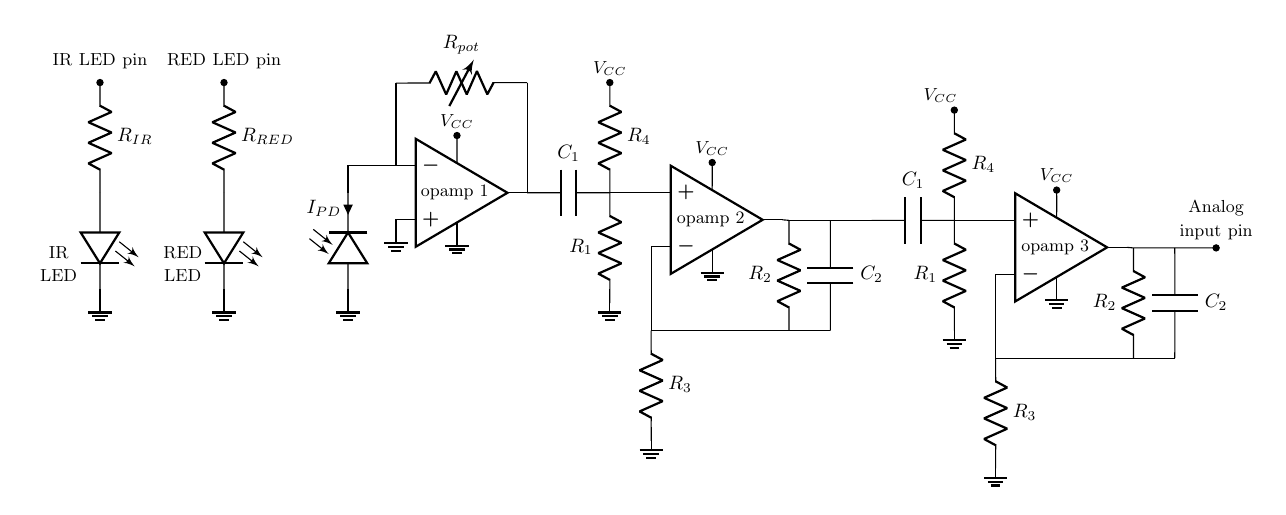
\begin{tikzpicture}[scale=0.7, transform shape]
		\draw (5.5, 8) to[american resistor, *-, l={$R_{IR}$}] (5.5, 6);
		\node[ground] at (5.5, 4.25){};
		\draw (5.5, 6) to[empty led] (5.5, 4);
		\draw (7.75, 8) to[american resistor, *-, l={$R_{RED}$}] (7.75, 6);
		\node[ground] at (7.75, 4.25){};
		\draw (7.75, 6) to[empty led] (7.75, 4);
		\node[shape=rectangle, minimum width=2.465cm, minimum height=0.715cm] at (5.5, 8.375){} node[anchor=north, align=center, text width=2.077cm, inner sep=6pt] at (5.5, 8.75){\small IR LED pin};
		\node[shape=rectangle, minimum width=2.465cm, minimum height=0.715cm] at (7.75, 8.375){} node[anchor=north, align=center, text width=2.077cm, inner sep=6pt] at (7.75, 8.75){\small RED LED pin};
		\draw (10, 4) to[empty photodiode, i^<=$I_{PD}$, current/distance=0.6] (10, 6);
		\node[ground] at (10, 4.25){};
		\node[op amp] at (12.06, 6){\small opamp 1};
		\node[ground] at (10.87, 5.51){};
		\draw (10, 6) |- (10.87, 6.49);
		\draw (10.87, 7.99) to[variable american resistor, l={$R_{pot}$}] (13.25, 8);
		\draw (13.25, 6) to[capacitor, l={$C_1$}] (14.75, 6);
		\draw (14.75, 6) to[american resistor, -*, l_={$R_4$}] (14.75, 8);
		\draw (14.75, 6) to[american resistor, l_={$R_1$}] (14.75, 4);
		\node[op amp, yscale=-1] at (16.69, 5.51){} node[anchor=center] at (16.58, 5.51) {\small opamp 2};
		\node[ground] at (14.75, 4.25){};
		\draw (10.87, 7.99) -| (10.87, 6.49);
		\draw (13.25, 8) -| (13.25, 6);
		\draw (14.75, 6) -- (15.5, 6);
		\node[ground] at (11.977, 5.461){};
		\draw (11.977, 6.539) to[short, -*] (11.977, 7.039);
		\node[shape=rectangle, minimum width=1.215cm, minimum height=0.426cm] at (11.977, 7.269){} node[anchor=north, align=center, text width=1.109cm, inner sep=2pt] at (11.977, 7.5){\small $V_{CC}$};
		\node[shape=rectangle, minimum width=1.215cm, minimum height=0.426cm] at (14.75, 8.23){} node[anchor=north, align=center, text width=1.109cm, inner sep=2pt] at (14.75, 8.461){\small $V_{CC}$};
		\node[ground] at (16.607, 4.971){};
		\draw (16.607, 6.049) to[short, -*] (16.607, 6.549);
		\node[shape=rectangle, minimum width=1.215cm, minimum height=0.426cm] at (16.607, 6.779){} node[anchor=north, align=center, text width=1.109cm, inner sep=2pt] at (16.607, 7.01){\small $V_{CC}$};
		\draw (18, 5.5) to[american resistor, l_={$R_2$}] (18, 3.5);
		\draw (18.75, 5.5) to[capacitor, l={$C_2$}] (18.75, 3.5);
		\draw (15.5, 3.5) to[american resistor, l={$R_3$}] (15.5, 1.5);
		\node[ground] at (15.5, 1.75){};
		\draw (15.5, 5.02) -- (15.5, 3.5);
		\draw (18.75, 3.5) -- (15.5, 3.5);
		\draw (19.5, 5.5) to[capacitor, l={$C_1$}] (21, 5.5);
		\draw (21, 5.5) to[american resistor, -*, l_={$R_4$}] (21, 7.5);
		\draw (21, 5.5) to[american resistor, l_={$R_1$}] (21, 3.5);
		\node[op amp, yscale=-1] at (22.94, 5.01){} node[anchor=center] at (22.83, 5.01) {\small opamp 3};
		\node[ground] at (21, 3.75){};
		\draw (21, 5.5) -- (21.75, 5.5);
		\node[shape=rectangle, minimum width=1.215cm, minimum height=0.426cm] at (20.75, 7.73){} node[anchor=north, align=center, text width=1.109cm, inner sep=2pt] at (20.75, 7.961){\small $V_{CC}$};
		\node[ground] at (22.857, 4.471){};
		\draw (22.857, 5.549) to[short, -*] (22.857, 6.049);
		\node[shape=rectangle, minimum width=1.215cm, minimum height=0.426cm] at (22.857, 6.279){} node[anchor=north, align=center, text width=1.109cm, inner sep=2pt] at (22.857, 6.51){\small $V_{CC}$};
		\draw (24.25, 5) to[american resistor, l_={$R_2$}] (24.25, 3);
		\draw (25, 5) to[capacitor, l={$C_2$}] (25, 3);
		\draw (21.75, 3) to[american resistor, l={$R_3$}] (21.75, 1);
		\node[ground] at (21.75, 1.25){};
		\draw (21.75, 4.52) -- (21.75, 3);
		\draw (25, 3) -- (21.75, 3);
		\draw (17.88, 5.51) to[short] (18, 5.5);
		\draw (18, 5.5) -- (19.5, 5.5);
		\draw (24.13, 5.01) to[short] (24.25, 5);
		\draw (24.25, 5) to[short, -*] (25.75, 5);
		\node[shape=rectangle, minimum width=1.465cm, minimum height=0.83cm] at (25.75, 5.5){} node[anchor=north, align=center, text width=1.359cm, inner sep=2pt] at (25.75, 5.933){\small Analog input pin};
		\node[shape=rectangle, minimum width=1.09cm, minimum height=1.09cm] at (7, 4.687){} node[anchor=north, align=center, text width=0.702cm, inner sep=6pt] at (7, 5.25){\small RED LED};
		\node[shape=rectangle, minimum width=1.09cm, minimum height=1.09cm] at (4.75, 4.687){} node[anchor=north, align=center, text width=0.702cm, inner sep=6pt] at (4.75, 5.25){\small IR LED};
	\end{tikzpicture}
\end{center}

\noindent
Circuit is composed by:
\begin{enumerate}
	\item two LEDs (red and infrared) connected in series with two resistors to limit the current through them, controlled by two digital
	pins of the Arduino board to turn them on and off
	\item a photodiode connected in reverse bias to a transimpedance amplifier (opamp 1) with a potentiometer in the feedback loop that
	converts the photodiode current into a voltage signal
	\item a passive high pass filter with a cutoff frequency of \(f_C \approx 0.8 \; Hz\) and a voltage offset of \(0.15 \; V\) (\(C_1\),
	\(R_1\) and \(R_4\)) to remove the DC component of the signal and apply a small positive offset to the signal to make it suitable
	for op amps with single positive power supply
	\item an active low pass filter with a cutoff frequency of \(f_C \approx 3 \; Hz\) and a gain of \(A_v = 11\) (opamp 2, \(R_2\), \(R_3\)
	and \(C_2\)) to filter the signal, remove high frequency noise and amplify the pulsation component of the signal
	\item a second passive high pass filter with offset (\(C_1\), \(R_1\) and \(R_4\))
	\item a second active low pass filter (opamp 3, \(R_2\), \(R_3\) and \(C_2\))
	\item the output terminal connected to an analog input pin of the Arduino board
\end{enumerate}

\subsubsection*{Oxygen saturation monitoring}
Oxygen saturation can be estimated by measuring the ratio of the pulsation component of the red and infrared signals, since oxygenated
and deoxygenated hemoglobin have different light absorption coefficients for red and infrared light. The ratio can be computed with the
following formula:
\[R = \frac{\displaystyle \left(\frac{AC}{DC}\right)_{RED}}{\displaystyle \left(\frac{AC}{DC}\right)_{IR}} = \frac{\displaystyle \frac{V_{\text{max, RED}} - V_{\text{min, RED}}}{V_{\text{min, RED}}}}{\displaystyle \frac{V_{\text{max, IR}} - V_{\text{min, IR}}}{V_{\text{min, IR}}}} \qquad\qquad \text{SpO}_2 = 97.94 + 1.15 \cdot R\]

\end{document}
